\documentclass[aps,prb,reprint,amsmath,amssymb,floatfix]{revtex4-2}
\usepackage{graphicx}
\usepackage{dcolumn}
\usepackage{bm}
\usepackage{booktabs}
\usepackage{multirow}
\usepackage{array}
\usepackage{hyperref}
\usepackage{natbib}
\usepackage{amsmath}

\providecommand{\tightlist}{\setlength{\itemsep}{0pt}\setlength{\parskip}{0pt}}
\providecommand{\pandocbounded}[1]{#1}
%DIF PREAMBLE EXTENSION ADDED BY LATEXDIFF
%DIF CFONT PREAMBLE %DIF PREAMBLE
\RequirePackage{color}\definecolor{RED}{rgb}{1,0,0}\definecolor{BLUE}{rgb}{0,0,1} %DIF PREAMBLE
\DeclareOldFontCommand{\sf}{\normalfont\sffamily}{\mathsf} %DIF PREAMBLE
\providecommand{\DIFaddtex}[1]{{\protect\color{blue} #1}} %DIF PREAMBLE
\providecommand{\DIFdeltex}[1]{} %DIF PREAMBLE
%DIF SAFE PREAMBLE %DIF PREAMBLE
\providecommand{\DIFaddbegin}{} %DIF PREAMBLE
\providecommand{\DIFaddend}{} %DIF PREAMBLE
\providecommand{\DIFdelbegin}{} %DIF PREAMBLE
\providecommand{\DIFdelend}{} %DIF PREAMBLE
\providecommand{\DIFmodbegin}{} %DIF PREAMBLE
\providecommand{\DIFmodend}{} %DIF PREAMBLE
%DIF FLOATSAFE PREAMBLE %DIF PREAMBLE
\providecommand{\DIFaddFL}[1]{\DIFadd{#1}} %DIF PREAMBLE
\providecommand{\DIFdelFL}[1]{\DIFdel{#1}} %DIF PREAMBLE
\providecommand{\DIFaddbeginFL}{} %DIF PREAMBLE
\providecommand{\DIFaddendFL}{} %DIF PREAMBLE
\providecommand{\DIFdelbeginFL}{} %DIF PREAMBLE
\providecommand{\DIFdelendFL}{} %DIF PREAMBLE
%DIF HYPERREF PREAMBLE %DIF PREAMBLE
\providecommand{\DIFadd}[1]{\texorpdfstring{\DIFaddtex{#1}}{#1}} %DIF PREAMBLE
\providecommand{\DIFdel}[1]{\texorpdfstring{\DIFdeltex{#1}}{}} %DIF PREAMBLE
%DIF LISTINGS PREAMBLE %DIF PREAMBLE
\RequirePackage{listings} %DIF PREAMBLE
\RequirePackage{color} %DIF PREAMBLE
\lstdefinelanguage{DIFcode}{ %DIF PREAMBLE
%DIF DIFCODE_CFONT %DIF PREAMBLE
  moredelim=[il][\color{red}\scriptsize]{\%DIF\ <\ }, %DIF PREAMBLE
  moredelim=[il][\color{blue}\sffamily]{\%DIF\ >\ } %DIF PREAMBLE
} %DIF PREAMBLE
\lstdefinestyle{DIFverbatimstyle}{ %DIF PREAMBLE
	language=DIFcode, %DIF PREAMBLE
	basicstyle=\ttfamily, %DIF PREAMBLE
	columns=fullflexible, %DIF PREAMBLE
	keepspaces=true %DIF PREAMBLE
} %DIF PREAMBLE
\lstnewenvironment{DIFverbatim}{\lstset{style=DIFverbatimstyle}}{} %DIF PREAMBLE
\lstnewenvironment{DIFverbatim*}{\lstset{style=DIFverbatimstyle,showspaces=true}}{} %DIF PREAMBLE
%DIF END PREAMBLE EXTENSION ADDED BY LATEXDIFF

\begin{document}

\title{Special Optimal Thermal Cell: \DIFdelbegin \DIFdel{First-Principles }\DIFdelend \DIFaddbegin \DIFadd{Correlator-Designed Supercells for Effective-Harmonic }\DIFaddend Phonons and Thermodynamics\DIFdelbegin \DIFdel{from Optimally Designed Minimal Supercells}\DIFdelend }

\author{Albert Linda}
\email{albert.hzbn@gmail.com}
\affiliation{Department of Materials Science and Engineering, Indian Institute of Technology, Kanpur}

\date{\today}

\begin{abstract}
\DIFdelbegin \DIFdel{We introduce }\DIFdelend \DIFaddbegin

\DIFadd{We introduce the }\DIFaddend Special Optimal Thermal Cell (SOTC), a \DIFdelbegin \DIFdel{self-consistent first-principles framework for computing temperature-renormalized phonon dispersions, heat capacities, zero-point energies (ZPE) , vibrational free energies, and, via quasi-harmonic coupling, continuous thermal expansion coefficients $\alpha(T)$ and isobaric heat capacities $C_P(T)$, using a single small periodically repeated supercell per self-consistency iteration. By analogy with }\DIFdelend \DIFaddbegin \DIFadd{deterministic
displacement-design strategy for extracting effective second-order interatomic
force constants (IFCs) from small periodic supercells. Inspired by }\DIFaddend the
Special Quasirandom Structure \DIFdelbegin \DIFdel{(SQS) approach to chemical disorder, SOTC replaces stochastic thermal ensembles with purposefully designed displacement fields whose displacement--displacement correlators best match the quantum thermal correlators of the target system up to a spatial cutoff. Interatomic force constants are extracted by ridge regression on the single displaced cell, and self-consistency between correlators and force constants is achieved in typically 2--4 density-functional theory }\DIFdelend \DIFaddbegin \DIFadd{construction, SOTC chooses collective atomic
displacements by minimizing the mismatch between selected shell-averaged
displacement correlators of the cell and those of a harmonic trial model. A
self-consistent cycle updates the trial phonons from density-functional-theory
}\DIFaddend (DFT) \DIFdelbegin \DIFdel{evaluations per system, one to two orders of magnitude fewer than the Temperature-Dependent Effective Potential (TDEP) method for equivalent accuracy. We benchmark SOTC against experiment for nine structurally diverse materials: elemental face-centered cubic (FCC ) metals }\DIFdelend \DIFaddbegin \DIFadd{forces and ridge-regression IFC fits. For the nine systems studied here
(FCC }\DIFaddend Al, Ag, Au, and Cu; \DIFdelbegin \DIFdel{elemental body-centered cubic (BCC ) metals }\DIFdelend \DIFaddbegin \DIFadd{BCC }\DIFaddend Mo and W; and \DIFdelbegin \DIFdel{the ionic rocksalt compounds }\DIFdelend \DIFaddbegin \DIFadd{rocksalt }\DIFaddend NaCl, MgO, and PbTe\DIFdelbegin \DIFdel{. The computed spectral Debye temperatures and phonon dispersions reproduce all major branch features for all nine systems. For ionic compounds (NaCl, MgO, PbTe), the }\DIFdelend \DIFaddbegin \DIFadd{), the
reported self-consistency criterion is reached in 2--5 iterations. The
archived calculations use 1--8 displaced configurations per iteration and an
undisplaced reference, corresponding to 4--36 force evaluations rather than
one force evaluation per iteration.
The resulting effective-harmonic phonons give }\DIFaddend constant-volume heat \DIFdelbegin \DIFdel{capacity agrees with experiment to within $\sim5\%$ at the design temperature; }\DIFdelend \DIFaddbegin \DIFadd{capacities
within approximately 5\% of experiment for the ionic compounds at their design
temperatures and within 7\% for all nine materials }\DIFaddend at 300\,K\DIFdelbegin \DIFdel{all nine materials agree to within 7\%. For high-temperature metals($T_\text{des} = 1000$--$1500$\,K)}\DIFdelend \DIFaddbegin \DIFadd{. At the design
temperatures of the metals}\DIFaddend , the harmonic \DIFdelbegin \DIFdel{model underestimates experimental $C_V$ by
6--13\% at the design temperature, where supra-Dulong-Petit anharmonic and electronic contributions dominate.  For aluminum, the }\DIFdelend \DIFaddbegin \DIFadd{heat capacity cannot reproduce
electronic and explicit anharmonic contributions above the Dulong--Petit
limit. The primary SOTC benchmarks assess second-order
effective-harmonic and }\DIFaddend quasi-harmonic \DIFdelbegin \DIFdel{extension yields a thermal expansion coefficient $\alpha(300\,\text{K}) = 36.9\times10^{-6}$ K$^{-1}$ with fewer than 7 total DFT evaluations.
The method is implemented in }\DIFdelend \DIFaddbegin \DIFadd{observables; they do not establish
equivalence to methods that sample explicit anharmonic free-energy surfaces.
In a separate 100-snapshot canonical validation for Al, NaCl, and W,
symmetry-constrained FC2+FC3+FC4 models reduce held-out force RMSE by
72--94\% relative to matched central finite-displacement phonopy FC2
baselines. This validates the higher-order fitting and export implementation,
not a few-configuration SOTC sampling advantage.  For NaCl, QE DFPT Born
charges and the electronic dielectric tensor produce a 2.895\,THz LO--TO
splitting when applied to the matched finite-displacement phonons.
The implementation is available as }\DIFaddend an open-source Python package interfaced
to Quantum ESPRESSO\DIFdelbegin \DIFdel{via a unified force-calculator.
}\DIFdelend \DIFaddbegin \DIFadd{.
}

\DIFaddend \end{abstract}

\maketitle

\section{Introduction}\label{introduction}

High-temperature phonon properties (renormalized dispersions, soft-mode
instabilities, thermal expansion, heat capacity) encode the anharmonic
response of a crystal to atomic vibrations with amplitudes reaching
several percent of the lattice constant. Accurate first-principles
descriptions of these properties are essential for predicting phase
stability \cite{ref1}, thermal conductivity \cite{ref2},
electron--phonon coupling \cite{ref3}, and thermodynamic databases for
materials design \cite{ref4}.

\DIFdelbegin \DIFdel{The predominant state-of-the-art methods for }\DIFdelend \DIFaddbegin \DIFadd{Finite-temperature lattice dynamics can be formulated at several distinct
levels. The temperature-dependent effective potential framework fits effective
second- and higher-order IFCs to }\DIFaddend finite-temperature force \DIFdelbegin \DIFdel{constants all require large supercells populated with displaced (or
MD-evolved) atomic configurations. The Temperature-Dependent Effective
Potential (TDEP) approach \cite{ref5,ref6} generates displacements from
a stochastic distribution matching the harmonic Bose--Einstein
statistics of a trial phonon model, and requires typically 30--100
independently displaced supercells of 54--512 atoms to converge the
interatomic force constants (IFCs). The Stochastic Self-Consistent
Harmonic Approximation (SSCHA) \cite{ref7,ref8} minimizes a variational
free energy over trial harmonic density matrices; its inner loop demands
$\sim$50--500 stochastic configurations per iteration}\DIFdelend \DIFaddbegin \DIFadd{data
\cite{ref5,ref6,ref10,ref52}. Variational self-consistent harmonic methods
optimize a trial distribution and its free energy \cite{ref7,ref8,ref50},
while mode-coupling theory provides a separate non-perturbative description of
anharmonic lattice dynamics \cite{ref51}}\DIFaddend . Ab initio molecular dynamics \DIFdelbegin \DIFdel{(AIMD) \cite{ref9} is exact in the classical limit
but requires picosecond trajectories on hundreds-of-atom cells and is
largely prohibitive at the cost of hybrid or meta-GGA functionals. Even
the most efficient variants, including compact TDEP \cite{ref10} and
on-the-fly machine learning \cite{ref11}, involve at minimum dozens of
DFT force evaluations per temperature point}\DIFdelend \DIFaddbegin \DIFadd{samples
classical nuclear trajectories on the chosen electronic potential-energy
surface \cite{ref9}. These approaches do not target identical observables or
approximations; meaningful cost or accuracy comparisons therefore require
matched cells, electronic settings, temperatures, and physical outputs}\DIFaddend .

In a parallel development, Zunger and coworkers \cite{ref12}
demonstrated that a random substitutional alloy can be mimicked
statistically by a single small supercell, the Special Quasirandom
Structure (SQS), whose chemical correlation functions match those of the
ideal random alloy up to a spatial cutoff. The key observation is that
structure encodes information: the correct spatial correlations are
imposed by construction rather than recovered by averaging over an
ensemble.

We apply \DIFdelbegin \DIFdel{this idea directly to the thermal problem. A thermally excited
crystal has well-defined }\DIFdelend \DIFaddbegin \DIFadd{the special-structure idea to displacement design. A harmonic trial
model defines }\DIFaddend displacement--displacement \DIFdelbegin \DIFdel{correlation
functions \(C_{ij}^{\alpha\beta}(\mathbf{R},T)\) that can be computed
accurately from a harmonic trial
phonon model using the exact quantum
formula. We show that there exists a small periodic
supercell (the SOTC)
whose atoms are displaced from equilibrium in a purposefully designed
pattern such that the cell's pair correlators match
\(C_{ij}^{\alpha\beta}\) to a prescribed cutoff\(r_\text{cut}\)}\DIFdelend \DIFaddbegin \DIFadd{correlations
\(C_{ab}^{\alpha\beta}(\mathbf R,T)\). SOTC searches a fixed periodic
supercell for a collective displacement pattern whose selected shell-averaged
correlators approximate these targets up to the IFC cutoff}\DIFaddend . DFT forces on \DIFdelbegin \DIFdel{this single cell are used to extract temperature-renormalized
IFCs by ridge regression; a self-consistent loop between IFCs}\DIFdelend \DIFaddbegin \DIFadd{the
designed configuration are then used in a symmetry-constrained ridge fit of
second-order IFCs, and the fitted phonons update the target correlators. The
small iteration counts reported below are empirical observations for the
present benchmarks, not a proof that a single configuration identifies an
arbitrary IFC tensor.
}

\DIFadd{SOTC is thus a deterministic configuration-design }\DIFaddend and \DIFdelbegin \DIFdel{correlators converges in 2--8 DFT evaluations. }%DIFDELCMD <

%DIFDELCMD < %%%
\DIFdel{The
method differs from TDEP in a key respect: while TDEP uses many
random displacement configurations to statistically sample the
thermal
distribution, SOTC uses one (or a small ensemble of) deterministically
designed configurations that are optimal in the information-theoretic
sense of best representing the target correlator hierarchy in the
smallest possible cell.
It differs from SSCHA in that no variational minimization of a free-energy functional is required; convergence is
diagnosed by direct comparison of displacement correlators between
successive iterations}\DIFdelend \DIFaddbegin \DIFadd{effective-FC2 fitting
procedure. It does not minimize an anharmonic variational free energy or
generate a time trajectory. Its proposed distinction is the explicit
optimization of prescribed spatial correlator moments before the force
calculation, rather than a general replacement for ensemble or trajectory
methods}\DIFaddend .

This paper is organized as follows. Section II presents the theoretical
framework: thermal displacement correlators, the SOTC objective
function, IFC extraction by ridge regression, the self-consistency loop,
and the quasi-harmonic extension for continuous thermodynamic
properties. Section III describes computational details. Section IV
reports benchmarks for all nine materials, including thermal expansion
for aluminum (Sec. IV.F). Section V discusses the method's range of
validity, limitations, computational cost, and comparison with the
phonopy quasi-harmonic approximation (QHA). Section VI concludes.

\section{Theory}\label{theory}

\subsection{Thermal Displacement
Correlators}\label{thermal-displacement-correlators}

Consider a crystal with \DIFdelbegin \DIFdel{primitive cell containing }\DIFdelend \(n_b\) \DIFaddbegin \DIFadd{basis atoms and \(N_c=N_1N_2N_3\)
primitive cells, so that the supercell contains \(n_bN_c\) }\DIFaddend atoms\DIFdelbegin \DIFdel{,
repeated as an \(N_1 \times N_2 \times N_3\) supercell containing
\(N = n_b N_1 N_2 N_3\) atoms}\DIFdelend . Let
\DIFdelbegin \DIFdel{\(u_i^\alpha\) denote }\DIFdelend \DIFaddbegin \DIFadd{\(u_a^\alpha(\mathbf R)\) be }\DIFaddend the displacement of \DIFdelbegin \DIFdel{atom \(i\) in Cartesian direction \(\alpha\) from its
zero-temperature equilibrium position. In the harmonic approximation, the
time-averaged thermal two-point correlator }\DIFdelend \DIFaddbegin \DIFadd{basis atom \(a\) in cell
\(\mathbf R\). With the Fourier convention defined in Appendix~A, the
equal-time canonical correlator of a harmonic lattice }\DIFaddend is \cite{ref13}:

{\footnotesize
\DIFdelbegin \begin{align*}
\DIFdel{C_{ij}^{\alpha\beta}(\mathbf{R},T)
  }&\DIFdel{= \langle u_i^\alpha(\mathbf{0})\, u_j^\beta(\mathbf{R})\rangle_T \nonumber }\\
  &\DIFdel{= \frac{\hbar}{2N\sqrt{M_i M_j}} \sum_{\mathbf{q},s}
     \frac{e_i^{\alpha*}(\mathbf{q}s)\,e_j^{\beta}(\mathbf{q}s)}{\omega_{\mathbf{q}s}}
     \coth\!\left(\frac{\hbar\omega_{\mathbf{q}s}}{2k_BT}\right) e^{i\mathbf{q}\cdot\mathbf{R}} \tag{1}
}\end{align*}%DIFAUXCMD
\DIFdelend \DIFaddbegin \begin{align}
\DIFadd{C_{ab}^{\alpha\beta}(\mathbf{R},T)
  }&\DIFadd{= \langle u_a^\alpha(\mathbf{0})\, u_b^\beta(\mathbf{R})\rangle_T \nonumber }\\
  &\DIFadd{= \frac{\hbar}{2N_c\sqrt{M_a M_b}} \sum_{\mathbf{q},s}
     \frac{e_a^{\alpha*}(\mathbf{q}s)\,e_b^{\beta}(\mathbf{q}s)}{\omega_{\mathbf{q}s}}
     \coth\!\left(\frac{\hbar\omega_{\mathbf{q}s}}{2k_BT}\right)
     e^{-i\mathbf{q}\cdot\mathbf{R}} .
}\end{align}\DIFaddend
}

\DIFdelbegin \DIFdel{where \(\hbar\) is the reduced Planck constant, \(k_B\) is the
Boltzmann constant, \(\langle\cdot\rangle_T\) denotes the canonical
thermal average at temperature \(T\), \(\omega_{\mathbf{q}s}\) and \(e_i^\alpha(\mathbf{q}s)\) are the phonon frequencies and polarization
vectors of branch }\DIFdelend \DIFaddbegin \DIFadd{Here \(\mathbf q\) runs over the \(N_c\) wave vectors commensurate with the
Born--von K\'arm\'an cell, }\DIFaddend \(s\) \DIFdelbegin \DIFdel{at wavevector \(\mathbf{q}\), \(M_i\) is the mass of atom \(i\), and \(\mathbf{R}\) is }\DIFdelend \DIFaddbegin \DIFadd{labels a phonon branch, and }\DIFaddend the \DIFdelbegin \DIFdel{lattice translation vector
between unit cells.
}\DIFdelend \DIFaddbegin \DIFadd{polarization
vectors obey the normalization stated in Appendix~A. The remaining symbols
have their usual meanings. Equation~(1) is standard harmonic-lattice theory;
a derivation and the phase convention are given in Appendix~A.
}

\DIFaddend The \(\coth\) factor encodes the full quantum Bose--Einstein statistics,
smoothly interpolating between the zero-point limit (\(T\to 0\):
\(\coth\to 1\)) and the classical equipartition limit
(\(k_BT\gg\hbar\omega\): \(\coth\to 2k_BT/\hbar\omega\)).

\DIFdelbegin \DIFdel{The trace-averaged scalar pair correlator (with $R\equiv|\mathbf{R}|$) is :
}%DIFDELCMD <

%DIFDELCMD < %%%
\begin{displaymath}
\DIFdel{\bar{C}_2(R, T) = \frac{1}{3}\sum_\alpha C_{ii}^{\alpha\alpha}(\mathbf{R},T) \tag{2}
}\end{displaymath}%DIFAUXCMD
\DIFdelend \DIFaddbegin \DIFadd{To reduce the tensor correlator to the scalar target used in the present
implementation, let \(\mathcal S_R^{ab}\) denote the set of lattice vectors
belonging to the crystallographic shell of radius \(R\) for basis pair
\((a,b)\), with multiplicity \(N_R^{ab}\). The shell and Cartesian trace
average is defined by
}\begin{equation}
\DIFadd{\bar C_2^{ab}(R,T)=\frac{1}{3N_R^{ab}}
\sum_{\mathbf R'\in\mathcal S_R^{ab}}\sum_{\alpha}
C_{ab}^{\alpha\alpha}(\mathbf R',T).
}\end{equation}\DIFaddend
\DIFdelbegin %DIFDELCMD <

%DIFDELCMD < %%%
\DIFdel{and
the mean-square displacement (MSD) is the \(\mathbf{R}=\mathbf{0}\)
value:
}\DIFdelend \DIFaddbegin \DIFadd{Thus \(R\) labels a discrete neighbor shell; it is not a continuum spherical
average. Numerically equivalent distances are grouped using the distance
tolerance reported with the calculation inputs. Species/basis-pair channels
are retained separately. This scalar reduction discards anisotropic and
off-diagonal correlation information, a limitation discussed in Sec.~V.D.
}\DIFaddend

\DIFdelbegin \begin{displaymath}
\DIFdel{\langle u^2\rangle_T = \bar{C}_2(0,T) = \frac{\hbar}{6NM}\sum_{\mathbf{q},s} \frac{1}{\omega_{\mathbf{q}s}} \coth\!\left(\frac{\hbar\omega_{\mathbf{q}s}}{2k_BT}\right) \tag{3}
}\end{displaymath}%DIFAUXCMD
\DIFdelend \DIFaddbegin \DIFadd{For a monatomic cubic crystal, the on-site value is the one-component
isotropic displacement parameter
\(U_{\rm iso}=\frac{1}{3}\langle|\mathbf u|^2\rangle\):
}\begin{equation}
\DIFadd{U_{\rm iso}(T)=\bar C_2(0,T)=
\frac{\hbar}{6N_cM}\sum_{\mathbf q,s}
\frac{1}{\omega_{\mathbf q s}}
\coth\!\left(\frac{\hbar\omega_{\mathbf q s}}{2k_BT}\right).
}\end{equation}\DIFaddend
\DIFdelbegin %DIFDELCMD <

%DIFDELCMD < %%%
\DIFdel{Here \(M\) is the common atomic mass (monatomic crystal, \(M_i=M\)) ;
for multi-species crystals, the right-hand side }\DIFdelend \DIFaddbegin \DIFadd{Equation~(3) follows from the trace }\DIFaddend of Eq.~(\DIFdelbegin \DIFdel{3) is replaced
by the species-resolved
\(\frac{\hbar}{6NM_i}\sum_{\mathbf{q},s}\frac{|e_i^\alpha(\mathbf{q}s)|^2}{\omega_{\mathbf{q}s}}\coth(\cdots)\)
summed over atom \(i\) in the unit cell. The MSD determines the thermal
displacement amplitude
\(u_\text{rms}(T) = \sqrt{\langle u^2\rangle_T}\), which is
the natural
scale of displacements to apply in the SOTC cell}\DIFdelend \DIFaddbegin \DIFadd{1) and the polarization-vector
completeness relation. The total three-dimensional MSD is
\(3U_{\rm iso}\), while crystallographic Debye--Waller factors use
\(B=8\pi^2U_{\rm iso}\). For compounds, species-resolved displacements are
evaluated from the full eigenvector-weighted mode sum rather than a
species-averaged mass and the total DOS. The displacement norm used to design
a SOTC configuration is documented separately from this one-component
quantity to avoid a factor-of-three ambiguity}\DIFaddend .

\subsection{The SOTC Objective
Function}\label{the-sotc-objective-function}

Let \(\Omega\) be a candidate supercell of \(n\) atoms (with
\(n \ll N\)) and let \(\{\mathbf{u}_i\}\) be a set of atomic
displacements assigned to those atoms.
The \textbf{SOTC \DIFdelbegin \DIFdel{quality
functional}\DIFdelend \DIFaddbegin \DIFadd{objective function}\DIFaddend } measures \DIFdelbegin \DIFdel{how well the correlators of this single displaced
cell match the quantum thermal }\DIFdelend \DIFaddbegin \DIFadd{the mismatch between the
selected correlators of a finite displacement vector and the harmonic trial
}\DIFaddend targets:

\DIFdelbegin \begin{displaymath}
\DIFdel{\mathcal{Q}[\{\mathbf{u}_i\}] = \sum_{R\,:\,R<r_\text{cut}} w(R) \left[\bar{C}_{2}^\text{cell}(R) - \bar{C}_{2}(R,T)\right]^2 \tag{4}
}\end{displaymath}%DIFAUXCMD
\DIFdelend \DIFaddbegin \begin{equation}
\DIFadd{\mathcal{Q}(\mathbf{u}) = \sum_{a,b}\sum_{R<r_\text{cut}} w_{ab}(R)
\left[\bar{C}_{2,ab}^\text{cell}(R;\mathbf u)
- \bar{C}_{2,ab}(R,T)\right]^2 .
}\end{equation}\DIFaddend

\DIFdelbegin \DIFdel{where
\(\bar{C}_{2}^\text{cell}(R) = \frac{1}{N_p(R)}\sum_{(i,j):\,|R_{ij}|=R}\frac{1}{3}\sum_\alpha u_i^\alpha u_j^\alpha\)
is the scalar pair correlator of the SOTC cell averaged over all
\(N_p(R)\) pairs at shelldistance \(R\), \(r_\text{cut}\) is the IFC
cutoff radius, and \(w(R) = \exp(-R/\xi_T)\) is a distance weight with
thermal coherence length:
}%DIFDELCMD <

%DIFDELCMD < %%%
\begin{displaymath}
\DIFdel{\xi_T = \frac{\hbar\bar{v}_s}{\gamma k_B T} \tag{5}
}\end{displaymath}%DIFAUXCMD
\DIFdelend \DIFaddbegin \DIFadd{Here \(\bar C_{2,ab}^{\rm cell}\) is formed with the same shell, trace, and
species averaging as Eq.~(2), and \(r_{\rm cut}\) is the real-space IFC
cutoff. Equation~(4) is introduced in this work; its gradient is given in
Appendix~C. A positive distance weight may be chosen, for example
}\begin{equation}
\DIFadd{w_{ab}(R;\xi_w)=\exp(-R/\xi_w),
}\end{equation}\DIFaddend
\DIFdelbegin %DIFDELCMD <

%DIFDELCMD < %%%
\DIFdel{where \(\bar{v}_s\) is the average acoustic velocity and \(\gamma\) is
the Grüneisen parameter. The coherence length decreases as \(1/T\),
so
the optimal cell size scales as \(\xi_T\); SOTC is therefore most
efficient precisely where conventional methods are most expensive}\DIFdelend \DIFaddbegin \DIFadd{where \(\xi_w\) is a numerical weighting length whose adequacy must be tested
by cutoff and dispersion convergence. We do not identify \(\xi_w\) with a
universal phonon mean free path: a finite dynamical phonon lifetime does not,
by itself, prove exponential decay of an equal-time displacement correlator.
No lifetime-based exponential decay or universal
\(T^{-1}\)/\(T^{-3}\) scaling law is assumed in this formulation}\DIFaddend .

Minimization of \(\mathcal{Q}\) over the displacement field
\(\{\mathbf{u}_i\}\) subject to \(|\mathbf{u}_i| \leq u_\text{rms}(T)\)
is performed by gradient descent with random restarts. The initial guess
is the harmonic displacement pattern obtained by sampling each phonon
mode with amplitude
\(A_{\mathbf{q}s}^{(0)} = \sqrt{\hbar\coth(\hbar\omega_{\mathbf{q}s}/2k_BT)/2\omega_{\mathbf{q}s}}\).
The optimization adjusts mode amplitudes and phase relations to minimize
the correlator mismatch while keeping displacements physically bounded.

\subsection{IFC Extraction by Ridge
Regression}\label{ifc-extraction-by-ridge-regression}

\DIFdelbegin \DIFdel{Given the SOTC displacement field \(\{\mathbf{u}_i\}\) and the DFT
forces \(\{F_i^\alpha\}\) computed on this single configuration, the
second-order IFCs \(\Phi_{ij}^{\alpha\beta}\) are extracted by solving
the linear force-displacement relation :
}\DIFdelend \DIFaddbegin \DIFadd{Let \(F_i^\alpha(\mathbf u)\) and \(F_i^\alpha(\mathbf0)\) be forces on the
displaced and reference structures at the same cell. The response force
\(\Delta F_i^\alpha=F_i^\alpha(\mathbf u)-F_i^\alpha(\mathbf0)\) removes any
residual reference force. To harmonic order, the collective-displacement
relation with translational invariance written explicitly is
}\DIFaddend

\DIFdelbegin \begin{displaymath}
\DIFdel{F_i^\alpha = -\sum_{j,\beta} \Phi_{ij}^{\alpha\beta}\, u_j^\beta \tag{6}
}\end{displaymath}%DIFAUXCMD
\DIFdelend \DIFaddbegin \begin{equation}
\DIFadd{\Delta F_i^\alpha = -\sum_{j,\beta}
\Phi_{ij}^{\alpha\beta}\,(u_j^\beta-u_i^\beta)
+\mathcal O(u^2).
}\end{equation}\DIFaddend

This constitutes an underdetermined system when the number of IFC
parameters \(N_\text{IFC}\) exceeds \(3n\) (the dimension of the force
vector). We use Tikhonov (ridge) regression to stabilize the inversion:

\DIFdelbegin \begin{displaymath}
\DIFdel{\hat{\boldsymbol{\Phi}} = -\left(\mathbf{G}^T\mathbf{G} + \lambda\mathbf{I}\right)^{-1} \mathbf{G}^T \mathbf{F} \tag{7}
}\end{displaymath}%DIFAUXCMD
\DIFdelend \DIFaddbegin \begin{equation}
\DIFadd{\hat{\boldsymbol{\Phi}} = -\left(\mathbf{G}^T\mathbf{G} + \lambda\mathbf{I}\right)^{-1} \mathbf{G}^T \Delta\mathbf{F}.
}\end{equation}\DIFaddend

\DIFdelbegin \DIFdel{where \(\mathbf{G}\) is the displacement matrix mapping IFC parameters
to atomic forces, \(\mathbf{F}\) is the force vector}\DIFdelend \DIFaddbegin \DIFadd{The geometry matrix \(\mathbf G\) contains the relative displacements in
Eq.~(6), \(\Delta\mathbf F\) stacks the response forces}\DIFaddend , and \(\lambda\) is the
\DIFdelbegin \DIFdel{regularization strength (default \(\lambda = 10^{-3}\) eV/Å\(^2\)). Sensitivity tests across \(\lambda = 10^{-4}\)--\(10^{-2}\) eV/Å\(^2\)
yield \(< 0.5\%\) variation in \(C_V\) for all benchmark systems; the
well-conditioned regression (rank 81--162, Table~\ref{tab:1}) renders thermodynamic
results insensitive to
the specific choice within this range}\DIFdelend \DIFaddbegin \DIFadd{ridge parameter. Equation~(7) is standard Tikhonov regularization applied to
the symmetry-reduced force model; the constrained construction is detailed in
Appendix~D}\DIFaddend . The acoustic sum rule \DIFdelbegin \DIFdel{\(\sum_j \Phi_{ij}^{\alpha\beta} = 0\) is enforced }\DIFdelend \DIFaddbegin \DIFadd{is imposed }\DIFaddend as a hard \DIFdelbegin \DIFdel{constraint by projecting the IFC space prior to regression. For
collective SOTC configurations, where all atoms are simultaneously
displaced, the force equation takes the form
\(F_i^\alpha = -\sum_{j,\beta}\Phi_{ij}^{\alpha\beta}(u_j^\beta - u_i^\beta)\);
using relative displacements explicitly encodes the acoustic sum rule
and
is required in place of the bare displacement \(u_j^\beta\) of
single-atom finite-displacement schemes (see App. D). For high-symmetry
bond types (FCC nearest-neighbor, rocksalt nearest-neighbor), }\DIFdelend \DIFaddbegin \DIFadd{linear constraint, and
}\DIFaddend an optional central-force \DIFdelbegin \DIFdel{symmetry projection constrains \(\Phi_{ij}\) to
the form
\(A\hat{R}_\alpha\hat{R}_\beta + B(\delta_{\alpha\beta} - \hat{R}_\alpha\hat{R}_\beta)\), halving the number of free parameters and improving stability}\DIFdelend \DIFaddbegin \DIFadd{projection further reduces the parameter space.
These constraints, the finite cutoff, and ridge regularization are physical and
statistical priors, and their influence must be distinguished from information
provided by the DFT forces}\DIFaddend .

\DIFdelbegin \DIFdel{The IFC extraction rank (the number of linearly independent force
equations relative to
}\DIFdelend \DIFaddbegin \DIFadd{For one \(n\)-atom configuration, \(\mathbf G\) has \(3n\) rows and hence
algebraic rank no larger than \(3n\). Full identification requires the rank to
be compared with }\DIFaddend the number of \DIFdelbegin \DIFdel{parameters) is a key diagnostic. For
a 32-atom FCC cell with \(r_\text{cut} = 4.5\) Å and
symmetrize\_bonds=True, the rankis typically 81--162 (depending on $N_\text{ens}$), sufficient for a
well-conditioned fit}\DIFdelend \DIFaddbegin \DIFadd{independent IFC parameters after all symmetry
and sum-rule reductions. Ridge regularization stabilizes a rank-deficient fit
but does not create missing information. The validation therefore reports parameter counts, singular-value tolerance, rank, and condition number
for each actual matrix rather than asserting coverage from the iteration count
alone}\DIFaddend .

\subsection{Phonon Reconstruction}\label{phonon-reconstruction}

From the extracted IFCs \(\hat{\Phi}_{ij}^{\alpha\beta}(\mathbf{R})\),
the dynamical matrix is constructed as:

\DIFdelbegin \begin{displaymath}
\DIFdel{D_{ij}^{\alpha\beta}(\mathbf{q}) = \frac{1}{\sqrt{M_i M_j}} \sum_{\mathbf{R}} \hat{\Phi}_{ij}^{\alpha\beta}(\mathbf{R})\, e^{i\mathbf{q}\cdot\mathbf{R}} \tag{8}
}\end{displaymath}%DIFAUXCMD
\DIFdelend \DIFaddbegin \begin{equation}
\DIFadd{D_{ij}^{\alpha\beta}(\mathbf{q}) = \frac{1}{\sqrt{M_i M_j}} \sum_{\mathbf{R}} \hat{\Phi}_{ij}^{\alpha\beta}(\mathbf{R})\, e^{i\mathbf{q}\cdot\mathbf{R}}
}\end{equation}\DIFaddend

\DIFaddbegin \DIFadd{Equation~(8) is the standard Fourier construction of the harmonic dynamical
matrix from real-space IFCs \cite{ref13}; the retained real-space cutoff and
non-analytic polar correction determine its domain of validity.
}

\DIFaddend Phonon dispersion: the \(3n_b\) branches \(\omega_{\mathbf{q}s}\) follow
from eigenvalues of \(D(\mathbf{q})\), evaluated on a dense
Monkhorst--Pack grid. The phonon density of states (DOS) is obtained by
linear tetrahedron integration with Gaussian broadening \(\sigma = 0.1\)
THz.

Thermodynamic properties follow directly from the phonon DOS
\(g(\omega)\):

\DIFdelbegin \begin{displaymath}
\DIFdel{C_V(T) = k_B \int_0^{\omega_\text{max}} g(\omega) \left(\frac{\hbar\omega}{2k_BT}\right)^2 \sinh^{-2}\!\left(\frac{\hbar\omega}{2k_BT}\right) d\omega \tag{9}
}\end{displaymath}%DIFAUXCMD
\DIFdelend \DIFaddbegin \begin{equation}
\DIFadd{C_V(T) = k_B \int_0^{\omega_\text{max}} g(\omega) \left(\frac{\hbar\omega}{2k_BT}\right)^2 \sinh^{-2}\!\left(\frac{\hbar\omega}{2k_BT}\right) d\omega
}\end{equation}\DIFaddend

\DIFdelbegin \begin{displaymath}
\DIFdel{F_\text{vib}(T) = k_B T \int_0^{\omega_\text{max}} g(\omega) \ln\!\left[2\sinh\!\left(\frac{\hbar\omega}{2k_BT}\right)\right] d\omega \tag{10}
}\end{displaymath}%DIFAUXCMD
\DIFdelend \DIFaddbegin \begin{equation}
\DIFadd{F_\text{vib}(T) = k_B T \int_0^{\omega_\text{max}} g(\omega) \ln\!\left[2\sinh\!\left(\frac{\hbar\omega}{2k_BT}\right)\right] d\omega
}\end{equation}\DIFaddend

\DIFdelbegin \begin{displaymath}
\DIFdel{\text{ZPE} = \frac{\hbar}{2}\int_0^{\omega_\text{max}} g(\omega)\,\omega\, d\omega \tag{11}
}\end{displaymath}%DIFAUXCMD
\DIFdelend \DIFaddbegin \begin{equation}
\DIFadd{\text{ZPE} = \frac{\hbar}{2}\int_0^{\omega_\text{max}} g(\omega)\,\omega\, d\omega
}\end{equation}\DIFaddend

\DIFdelbegin \begin{displaymath}
\DIFdel{\text{MSD}(T) = \frac{\hbar}{2M} \int_0^{\omega_\text{max}} \frac{g(\omega)}{\omega} \coth\!\left(\frac{\hbar\omega}{2k_BT}\right) d\omega \tag{12}
}\end{displaymath}%DIFAUXCMD
\DIFdelend \DIFaddbegin \begin{equation}
\DIFadd{\begin{aligned}
U_{\rm iso}(T)
 &= \frac{\hbar}{6M}\int_0^{\omega_{\rm max}}
 \frac{g(\omega)}{\omega}
 \coth\!\left(\frac{\hbar\omega}{2k_BT}\right)d\omega,\\
\int_0^{\omega_{\rm max}}g(\omega)d\omega&=3 .
\end{aligned}
}\end{equation}\DIFaddend

\DIFdelbegin \DIFdel{where \(M\) is the atomic mass per formula-unit atom(valid for a
monatomic crystal, or as the }\DIFdelend \DIFaddbegin \DIFadd{Equation~(12) is the monatomic one-component displacement obtained from
Eq.~(3) when the total DOS is normalized to three modes per atom. For a
compound, species-resolved eigenvector weights and masses are required; a
}\DIFaddend species-averaged mass \DIFdelbegin \DIFdel{for a compound when
using }\DIFdelend \DIFaddbegin \DIFadd{multiplying }\DIFaddend the total DOS \DIFdelbegin \DIFdel{\(g(\omega)\) normalized per atom)}\DIFdelend \DIFaddbegin \DIFadd{is not used. The harmonic
thermodynamic identities in Eqs.~(9)--(12) are standard consequences of the
independent-phonon partition function \cite{ref13}}\DIFaddend .
The spectral Debye temperature is the second-moment Debye temperature
\DIFaddbegin

\DIFaddend \(T_D^\text{spec} = (\hbar/k_B)\sqrt{5\langle\omega^2\rangle_g/3}\),
where
\(\langle\omega^2\rangle_g = \int g(\omega)\,\omega^2\,d\omega/\int g(\omega)\,d\omega\)
is the mean-square phonon frequency over the DOS; this uses the Debye
relation \(\langle\omega^2\rangle = 3\omega_D^2/5\). The caloric Debye
temperature \(T_D^\text{cal}(T)\) is defined by inversion of the Debye
model for \(C_V(T)\).

\subsection{Self-Consistent Loop}\label{self-consistent-loop}

The SOTC method is closed into a self-consistency cycle:

\begin{enumerate}
\def\labelenumi{\arabic{enumi}.}
\tightlist
\item
  \textbf{Initialize}: start from a Debye or Einstein trial phonon model
  \(\omega^{(0)}(\mathbf{q})\).
\item
  \textbf{Compute target correlators}: \(\bar{C}_2(R,T)\) from Eqs.
  (1)--(2) using current phonon model.
\item
  \textbf{Design \DIFdelbegin \DIFdel{SOTC cell}\DIFdelend \DIFaddbegin \DIFadd{configurations}\DIFaddend }: with the supercell \DIFdelbegin \DIFdel{geometry fixed(see
  below),
  minimize \(\mathcal{Q}[\{\mathbf{u}_i\}]\) }\DIFdelend \DIFaddbegin \DIFadd{fixed,
  minimize \(\mathcal Q(\mathbf u)\) }\DIFaddend [Eq.\DIFaddbegin \DIFadd{~}\DIFaddend (4)] \DIFdelbegin \DIFdel{over
  the displacement field to obtain the optimal displaced configuration}\DIFdelend \DIFaddbegin \DIFadd{to generate
  \(N_{\rm ens}\) displacement configurations}\DIFaddend .
\item
  \textbf{DFT forces}: \DIFdelbegin \DIFdel{single-point calculation on the displaced SOTC
  cell}\DIFdelend \DIFaddbegin \DIFadd{evaluate the undisplaced reference
  and all \(N_{\rm ens}\) displaced configurations}\DIFaddend .
\item
  \textbf{Extract IFCs}: ridge regression from Eq. (6).
\item
  \textbf{Update phonon model}: diagonalize \(D(\mathbf{q})\) from new
  IFCs.
\item
  \textbf{Check convergence}: \DIFdelbegin \DIFdel{\(\|\Delta\bar{C}_2\|_2 < 10^{-4}\)
  }\DIFdelend \DIFaddbegin \DIFadd{the archived benchmarks use
  \(\|\Delta\bar C_2\|_2<3\times10^{-3}\)~}\DIFaddend Å\(^2\)\DIFaddbegin \DIFadd{, together with the
  material-specific minimum iteration counts reported in the calculation
  inputs}\DIFaddend . If not converged, \DIFdelbegin \DIFdel{go }\DIFdelend \DIFaddbegin \DIFadd{return }\DIFaddend to step 2.
\end{enumerate}

\DIFdelbegin \DIFdel{Each full iteration requires exactly one DFT force evaluation. Convergence is typically reached in 2--4 iterations for simple metals
and 2--8 iterations for transition metals and compounds with
soft modes
(see Sec. IV.
A).
}\DIFdelend \DIFaddbegin \DIFadd{The Debye or Einstein model supplies only the first target in the intended
self-consistent workflow; subsequent targets depend on the fitted
material-specific IFCs. Nevertheless, the finite-data priors and numerical
safeguards can retain initialization dependence. Validation requires comparison of Debye, Einstein, perturbed, and deliberately poor initial
models rather than assuming a unique fixed point.
}

\DIFadd{Each iteration evaluates \(N_{\rm ens}\) displaced configurations and an
undisplaced reference configuration. In the current implementation the
reference is recomputed once per iteration; hence the force-call count is
\(N_{\rm iter}(N_{\rm ens}+1)\), not \(N_{\rm iter}\). The archived benchmarks
reach their stopping criterion in 2--5 iterations with
\(N_{\rm ens}=1\)--8, as detailed in Table~I. Iteration count is therefore not
used as a proxy for DFT cost.
}\DIFaddend

\subsection{Quasi-Harmonic Approximation and Continuous High-Temperature
Properties}\label{quasi-harmonic-approximation-and-continuous-high-temperature-properties}

The self-consistent SOTC loop delivers converged IFCs
\(\Phi_{ij}^{*\alpha\beta}(T)\) at a single design temperature \(T\). To
obtain continuous thermodynamic properties, specifically the thermal
expansion coefficient \(\alpha(T)\), isobaric heat capacity \(C_P(T)\),
and bulk modulus \(B(T)\), across a temperature range without repeating
the SOTC loop at each \(T\), we couple SOTC phonons to the QHA.

\textbf{SOTC-QHA setup.} \DIFdelbegin \DIFdel{Three SOTC runs are performed at volumes
\(V_-, V_0, V_+\) with \(V_\pm = V_0(1 \pm \delta)\), where
\(\delta = 0.01\)--0.02 is a small volume perturbation. Three DFT static
energies \(E_0(V_\pm), E_0(V_0)\) are computed on the primitive cell
(negligible cost). The total }\DIFdelend \DIFaddbegin \DIFadd{A converged QHA calculation requires a set of
\(N_V\) volumes spanning the thermally sampled range. Static reference-lattice
energies \(E_0(V)\) and phonons are computed directly at every volume; energies
of thermally displaced configurations are not substituted for \(E_0\), and
IFCs at an uncalculated volume are not inferred by linear extrapolation. At
least five volumes are used for a third-order Birch--Murnaghan fit, with
convergence checked against the number and range of volumes. The zero-pressure
}\DIFaddend Helmholtz free energy is
\DIFdelbegin \DIFdel{:
}%DIFDELCMD <

%DIFDELCMD < %%%
\begin{displaymath}
\DIFdel{G(T,V) = E_0(V) + F_\text{vib}(T,V) \tag{13}
}\end{displaymath}%DIFAUXCMD
\DIFdelend \DIFaddbegin \begin{equation}
\DIFadd{F(T,V)=E_0(V)+F_{\rm vib}(T,V),
}\end{equation}\DIFaddend
\DIFdelbegin %DIFDELCMD <

%DIFDELCMD < %%%
\DIFdel{where \(E_0(V)\) is fitted to a parabolic (Birch-Murnaghan) equation of
state through the three volumes, and \(F_\text{vib}(T,V)\) is
interpolated quadratically in \(V\) from the three SOTC phonon
calculations:
}%DIFDELCMD <

%DIFDELCMD < %%%
\begin{displaymath}
\DIFdel{F_\text{vib}(T,V) = k_BT\sum_{\mathbf{q},s}\ln\!\left[2\sinh\!\left(\frac{\hbar\omega_{\mathbf{q}s}(V)}{2k_BT}\right)\right] \tag{14}
}\end{displaymath}%DIFAUXCMD
\DIFdelend \DIFaddbegin \DIFadd{where the harmonic vibrational contribution is
}\begin{equation}
\DIFadd{F_{\rm vib}(T,V)=k_BT\sum_{\mathbf q,s}
\ln\!\left[2\sinh\!\left(\frac{\hbar\omega_{\mathbf q s}(V)}{2k_BT}\right)\right].
}\end{equation}\DIFaddend
\DIFdelbegin %DIFDELCMD <

%DIFDELCMD < %%%
\DIFdel{At each temperature \(T\)}\DIFdelend \DIFaddbegin \DIFadd{At external pressure \(p\)}\DIFaddend , the equilibrium volume \DIFdelbegin \DIFdel{\(V^*(T)\) is found by
minimizing \(G(T,V)\) over \(V\):
}%DIFDELCMD <

%DIFDELCMD < %%%
\begin{displaymath}
\DIFdel{\frac{\partial G}{\partial V}\bigg|_{V^*(T)} = \frac{dE_0}{dV} + \frac{\partial F_\text{vib}}{\partial V} = 0 \tag{15}
}\end{displaymath}%DIFAUXCMD
\DIFdelend \DIFaddbegin \DIFadd{minimizes
\(F(T,V)+pV\):
}\begin{equation}
\DIFadd{\left.\frac{\partial [F(T,V)+pV]}{\partial V}\right|_{V^*(T,p)}=0 .
}\end{equation}\DIFaddend
\DIFdelbegin %DIFDELCMD <

%DIFDELCMD < %%%
\DIFdel{\textbf{Derived thermal quantities.} From \(V^*(T)\) and the curvature
of }\DIFdelend \DIFaddbegin \DIFadd{Thus \(F\), rather than }\DIFaddend \(G\)\DIFdelbegin \DIFdel{:
}\DIFdelend \DIFaddbegin \DIFadd{, is minimized at \(p=0\). Equations
(13)--(15) are the standard quasi-harmonic construction \cite{ref44,ref45};
they do not imply an anharmonic variational upper bound.
}\DIFaddend

\DIFdelbegin \begin{displaymath}
\DIFdel{\alpha(T) = \frac{1}{V^*}\frac{dV^*}{dT}, \qquad B(T) = -V^*\frac{\partial^2 G}{\partial V^2}\bigg|_{V^*} \tag{16}
}\end{displaymath}%DIFAUXCMD
\DIFdelend \DIFaddbegin \DIFadd{For a cubic crystal, define the volumetric and linear expansion coefficients
separately. The thermodynamic identities are
}\begin{equation}
\DIFadd{\alpha_V=\frac{1}{V^*}\frac{dV^*}{dT},\qquad
\alpha_L=\frac{\alpha_V}{3},\qquad
B_T=V^*\left.\frac{\partial^2F}{\partial V^2}\right|_{V^*}.
}\end{equation}\DIFaddend
\DIFdelbegin %DIFDELCMD <

%DIFDELCMD < %%%
\begin{displaymath}
\DIFdel{C_P(T) = C_V(T) + TV^*(T)\,\alpha(T)^2\,B(T) \tag{17}
}\end{displaymath}%DIFAUXCMD
\DIFdelend \DIFaddbegin \DIFadd{The corresponding heat-capacity relation is
}\begin{equation}
\DIFadd{C_P-C_V=TV^*B_T\alpha_V^2
       =9TV^*B_T\alpha_L^2 .
}\end{equation}\DIFaddend
\DIFaddbegin \DIFadd{The positive curvature sign, the distinction between \(\alpha_V\) and
\(\alpha_L\), and the factor of nine in the linear-coefficient form are
essential. All numerical QHA results must be regenerated with these conventions
and with a converged volume grid before an accuracy or cost comparison is made.
}\DIFaddend

\DIFdelbegin \DIFdel{where \(C_V(T)\) uses the SOTC phonons at \(V^*(T)\) via Eq. (9). The
total DFT cost of SOTC-QHA is \(3N_\text{iter}\) SOTC evaluations plus 3
primitive-cell static self-consistent field (SCF) calculations,
approximately \(3\times\) the per-temperature cost of a single SOTC run, compared to $\sim165\times$ for a full phonopy-QHA thermal
expansion calculation at equivalent supercell size and
k-point density. }%DIFDELCMD <

%DIFDELCMD < %%%
\DIFdelend \textbf{Grüneisen shortcut.} When volume-changing DFT runs are not
desired, a faster estimate uses the mode Grüneisen parameters:

\DIFdelbegin \begin{displaymath}
\DIFdel{\gamma_{\mathbf{q}s} = -\frac{V}{\omega_{\mathbf{q}s}}\frac{\partial\omega_{\mathbf{q}s}}{\partial V}\bigg|_{V_0} \approx -\frac{V_0}{\omega_{\mathbf{q}s}}\frac{\omega_{\mathbf{q}s}(V_+)-\omega_{\mathbf{q}s}(V_-)}{V_+-V_-} \tag{18}
}\end{displaymath}%DIFAUXCMD
\DIFdelend \DIFaddbegin \begin{equation}
\DIFadd{\gamma_{\mathbf{q}s} = -\frac{V}{\omega_{\mathbf{q}s}}\frac{\partial\omega_{\mathbf{q}s}}{\partial V}\bigg|_{V_0} \approx -\frac{V_0}{\omega_{\mathbf{q}s}}\frac{\omega_{\mathbf{q}s}(V_+)-\omega_{\mathbf{q}s}(V_-)}{V_+-V_-}
}\end{equation}\DIFaddend

The heat-capacity-weighted average
\(\gamma_\text{eff}(T) = \sum_{\mathbf{q}s}c_{\mathbf{q}s}(T)\gamma_{\mathbf{q}s}/\sum_{\mathbf{q}s}c_{\mathbf{q}s}(T)\)
gives:

\DIFdelbegin \begin{displaymath}
\DIFdel{\alpha(T) \approx \frac{\gamma_\text{eff}(T)\,C_V(T)}{3\,B_0\,V_0} \tag{19}
}\end{displaymath}%DIFAUXCMD
\DIFdelend \DIFaddbegin \begin{equation}
\DIFadd{\alpha_L(T) \approx
\frac{\gamma_\text{eff}(T)\,C_V(T)}{3B_0V_0},\qquad
\alpha_V(T)=3\alpha_L(T).
}\end{equation}\DIFaddend

\DIFdelbegin \DIFdel{where \(B_0 = V_0(\partial^2 E_0/\partial V^2)|_{V_0}\) is the }\DIFdelend \DIFaddbegin \DIFadd{Here \(B_0=V_0(\partial^2E_0/\partial V^2)_{V_0}\) is the positive }\DIFaddend static
bulk modulus. \DIFdelbegin \DIFdel{Both methods are implemented in the \texttt{SOTCQuasiHarmonic} class; the full QHA is more accurate above
\(0.8\,T_\text{melt}\), while the }\DIFdelend \DIFaddbegin \DIFadd{Equation~(19) is the standard cubic }\DIFaddend Grüneisen \DIFdelbegin \DIFdel{shortcut requires no
additional volume minimization loop}\DIFdelend \DIFaddbegin \DIFadd{relation
\cite{ref44}; it requires volume derivatives of the phonons and is a diagnostic
approximation, not an independent validation of QHA. Software-specific class
names and keyword choices are moved to the reproducibility material}\DIFaddend .

\section{Computational Details}\label{computational-details}

\subsection{DFT Calculations}\label{dft-calculations}

All \DIFdelbegin \DIFdel{DFT }\DIFdelend \DIFaddbegin \DIFadd{force }\DIFaddend calculations used Quantum ESPRESSO \DIFdelbegin \DIFdel{(QE) \cite{ref46} version
}\DIFdelend 7.5 \DIFdelbegin \DIFdel{, interfaced through the SOTC unified force-calculator API using the
\texttt{pw.x} total-energy/force driver. The Perdew-Burke-Ernzerhof
(PBE
) generalized gradient approximation (GGA) \cite{ref17}was used
throughout. Pseudopotentials were drawn from the Standard Solid-State
Pseudopotentials (SSSP ) }\DIFdelend \DIFaddbegin \DIFadd{\cite{ref46}, PBE
\cite{ref17}, and pseudopotentials from the SSSP }\DIFaddend efficiency library
\cite{ref47}\DIFdelbegin \DIFdel{: norm-conserving ONCV pseudopotentials for Ag(\texttt{Ag\_ONCV\_PBE-1.0}), Au(\texttt{Au\_ONCV\_PBE-1.0})}\DIFdelend \DIFaddbegin \DIFadd{. The selected potentials were ONCV for Ag}\DIFaddend , \DIFaddbegin \DIFadd{Au, }\DIFaddend and Mo\DIFdelbegin \DIFdel{(\texttt{Mo\_ONCV\_PBE-1.0}); projector augmented-wave (PAW ) pseudopotentials for
Al(\texttt{Al.pbe-n-kjpaw\_psl.1.0.0}), Cu(\texttt{Cu.paw.z\_11.ld1.psl.v1.0.0-low}), Mg(\texttt{Mg.pbe-n-kjpaw\_psl.0.3.0}), O(\texttt{O.pbe-n-kjpaw\_psl.0.1})}\DIFdelend \DIFaddbegin \DIFadd{; PAW for
Al}\DIFaddend , \DIFaddbegin \DIFadd{Cu, Mg, O, }\DIFaddend and Pb\DIFdelbegin \DIFdel{(\texttt{Pb.pbe-dn-kjpaw\_psl.0.2.2})}\DIFdelend ; and ultrasoft \DIFdelbegin \DIFdel{Vanderbilt
pseudopotentials (USPP) for Cl (\texttt{cl\_pbe\_v1.4.uspp.F}), Na(\texttt{na\_pbe\_v1.5.uspp.F}), Te (\texttt{Te\_pbe\_v1.uspp.F})}\DIFdelend \DIFaddbegin \DIFadd{for Na}\DIFaddend , \DIFaddbegin \DIFadd{Cl, Te, }\DIFaddend and W\DIFdelbegin \DIFdel{(\texttt{W\_pbe\_v1.2.uspp.F}). Plane-wave kinetic-energy cutoffs (ecutwfc) : }\DIFdelend \DIFaddbegin \DIFadd{. Wave-function
cutoffs (Ry) were }\DIFaddend Al 40\DIFdelbegin \DIFdel{Ry}\DIFdelend , Ag 50\DIFdelbegin \DIFdel{Ry}\DIFdelend , Au 45\DIFdelbegin \DIFdel{Ry}\DIFdelend , Cu 45\DIFdelbegin \DIFdel{Ry}\DIFdelend , Mo 40\DIFdelbegin \DIFdel{Ry, }\DIFdelend \DIFaddbegin \DIFadd{, W 30, }\DIFaddend NaCl 60\DIFdelbegin \DIFdel{Ry
(Cl drives the cutoff)}\DIFdelend ,
MgO 80\DIFdelbegin \DIFdel{Ry (O drives the cutoff), PbTe 44 Ry (Pb
drives the cutoff), W 30 Ry. }\DIFdelend \DIFaddbegin \DIFadd{, and PbTe 44. }\DIFaddend Charge-density cutoffs \DIFdelbegin \DIFdel{(ecutrho) were set
to \(4\times\) ecutwfc for NC ONCV pseudopotentials and \(8\times\)
ecutwfc for PAWand USPP pseudopotentials. Brillouin zone sampling used
a \(\Gamma\)-centered \(2\times2\times2\) Monkhorst--Pack grid for }\DIFdelend \DIFaddbegin \DIFadd{were four times the
wave-function cutoff for ONCV and eight times it for PAW/ultrasoft
potentials. }\DIFaddend FCC and BCC supercells \DIFdelbegin \DIFdel{; a \(\Gamma\)-point-only (\(1\times1\times1\)) grid
was used for the rocksalt supercells (NaCl, MgO, PbTe), where the
64-atom cell provides sufficient Brillouin zone folding. Electronic
smearing used
the }\DIFdelend \DIFaddbegin \DIFadd{used a Gamma-centered
\(2\times2\times2\) k mesh; rocksalt supercells used Gamma only. Metals used
}\DIFaddend Marzari--Vanderbilt \DIFdelbegin \DIFdel{cold-smearing scheme \cite{ref18} with degauss \(= 0.02\) Ryfor metals, and fixed occupationsfor
insulators (NaCl, MgO, PbTe). Ionic relaxation was not performed; all
force evaluations are }\DIFdelend \DIFaddbegin \DIFadd{cold smearing \cite{ref18} of 0.02\,Ry, while the
insulators used fixed occupations. Literal pseudopotential filenames, QE
keywords, and software class/flag names are collected in Appendix~K rather
than the theory section.
}

\DIFadd{Experimental lattice constants and ideal high-symmetry fractional coordinates
were used for the archived benchmarks. An undisplaced }\DIFaddend single-point \DIFdelbegin \DIFdel{calculations on the SOTC-designed
displaced geometry. }\DIFdelend \DIFaddbegin \DIFadd{calculation
at the same cell defines the reference force and stress. IFC fits use
\(\Delta\mathbf F=\mathbf F(\mathbf u)-\mathbf F(\mathbf0)\), as in Eq.~(6),
rather than assuming \(\mathbf F(\mathbf0)=0\). The calculation archive should report
maximum/RMS reference forces, induced-force scales, residual stresses, and
comparisons with representative PBE-relaxed cells.
}\DIFaddend

\subsection{SOTC Supercell Setup}\label{sotc-supercell-setup}

The supercell geometry (Hermite Normal Form matrix \(\mathbf{H}\)) is
selected once before the self-consistency loop by enumerating all HNF
candidates whose number of primitive cells \(n\) satisfies
\(\max(2,\,n_\text{sc}-2) \le n \le n_\text{sc}\), where
\(n_\text{sc}\) is the user-specified target. Candidates are ranked by a
two-criterion score: nearest-neighbor shell completeness first, then
supercell lattice condition number (a measure of cell cubicity); the best candidate at or below the
target size is adopted. This upper bound ensures the supercell never
exceeds the intended size.

FCC metals (Al, Ag, Au, Cu) used a \(2\times2\times2\) conventional-cell
supercell (4 atoms/cell \(\times\) 8 = 32 atoms); BCC metals (Mo, W)
used a 64-atom supercell (2 atoms/cell \(\times\) 32 conventional cells)
and rocksalt compounds (NaCl, MgO, PbTe) used a \(2\times2\times2\)
conventional-cell supercell (8 atoms/cell \(\times\) 8 = 64 atoms).
\DIFdelbegin \DIFdel{Experimental lattice parameters were used for all systems (Table~\ref{tab:1})}\DIFdelend \DIFaddbegin

\DIFadd{The experimental lattice parameters are provided in the archived inputs; Table~I
now reports force-call accounting}\DIFaddend . The IFC \DIFdelbegin \DIFdel{cutoff radius \(r_\text{cut}\) was set to include all pairs within
the 4th neighbor shell (Table~\ref{tab:2}). Ridge regularization
\(\lambda = 10^{-3}\) eV/Å\(^2\). Central-force symmetry }\DIFdelend \DIFaddbegin \DIFadd{cutoffs are listed in Table~I, and
the ridge parameter was \(10^{-3}\) in the code's reported units. A
central-force bond }\DIFaddend projection was enabled for all \DIFdelbegin \DIFdel{systems (\texttt{symmetrize\_bonds=True}). All benchmark calculations used a single }\DIFdelend \DIFaddbegin \DIFadd{archived benchmarks. Because
this is a strong physical prior rather than a software detail, sensitivity tests should compare it with the less constrained tensor fit.
}

\DIFadd{The archived benchmark workflow used one }\DIFaddend SOTC displacement configuration per
\DIFdelbegin \DIFdel{iteration
(\(N_\text{ens} = 1\)), sufficient because the representability theorem
(App. E) guarantees }\DIFdelend \DIFaddbegin \DIFadd{self-consistency iteration (\(N_{\rm ens}=1\)). This fact does not guarantee
}\DIFaddend full IFC coverage\DIFdelbegin \DIFdel{for the supercell sizes and cutoffs used here}\DIFdelend \DIFaddbegin \DIFadd{. For every benchmark, the data release should report
the dimensions and numerical rank of the symmetry-reduced design matrix, its
singular-value threshold and condition number, and the independent parameter
count}\DIFaddend . The ensemble mode (\DIFdelbegin \DIFdel{\(N_\text{ens} > 1\)) is available
for 3IFC extraction (Sec.
V.C) but was not used in these benchmarks.
}\DIFdelend \DIFaddbegin \DIFadd{\(N_{\rm ens}>1\)) provides additional force rows
when an overdetermined fit is required.
}\DIFaddend

\subsection{Phonon Post-Processing}\label{phonon-post-processing}

Phonon \DIFdelbegin \DIFdel{dispersions were computed on }\DIFdelend \DIFaddbegin \DIFadd{DOS calculations used }\DIFaddend a \(30\times30\times30\) Monkhorst--Pack \DIFdelbegin \DIFdel{grid }\DIFdelend \DIFaddbegin \DIFadd{mesh
}\DIFaddend (27,000 \DIFdelbegin \DIFdel{q-points)interpolated via }\DIFdelend \DIFaddbegin \DIFadd{q points), while band dispersions were interpolated from }\DIFaddend the real-space
IFCs \DIFdelbegin \DIFdel{, using band paths }\DIFdelend \DIFaddbegin \DIFadd{along the paths stored with the released band data:
}\DIFaddend \(\Gamma\)\DIFdelbegin \DIFdel{-X-K-}\DIFdelend \DIFaddbegin \DIFadd{-X-W-K-}\DIFaddend \(\Gamma\)-L for FCC \DIFdelbegin \DIFdel{,
}\DIFdelend \DIFaddbegin \DIFadd{and rocksalt and
}\DIFaddend \(\Gamma\)\DIFdelbegin \DIFdel{-H-P-}\DIFdelend \DIFaddbegin \DIFadd{-H-N-}\DIFaddend \(\Gamma\)\DIFdelbegin \DIFdel{-N for BCC, and \(\Gamma\)-X-U-\(\Gamma\)-L-K
for rocksalt}\DIFdelend \DIFaddbegin \DIFadd{-P-H for BCC}\DIFaddend . Thermal properties were computed on an
\(8\times8\times8\)
\DIFaddbegin

\DIFaddend grid (512 q-points) for \(C_V(T)\), \(F_\text{vib}(T)\), and
\(S_\text{vib}(T)\). Gaussian broadening \(\sigma = 0.1\) THz was
applied to the phonon DOS. Convergence of \(C_V\) with q-mesh was
verified by comparing \(8\times8\times8\) and \(16\times16\times16\)
grids for Al and MgO; the difference is \(< 0.05\) J/(mol·K) in both
cases, confirming that the \(8\times8\times8\) grid is fully converged.

\subsection{Experimental Reference
Data}\label{experimental-reference-data}

Experimental Debye temperatures and heat capacities were taken from the
NIST-JANAF tables \cite{ref20} and Kittel \cite{ref21}. References for
individual systems: Al \cite{ref22,ref23}, Ag \cite{ref23}, Au
\cite{ref24}, Cu \cite{ref25}, Mo \cite{ref26,ref27}, W \cite{ref27},
NaCl \cite{ref28}, MgO \cite{ref29,ref30}, PbTe \cite{ref31,ref32}. For
comparison of phonon dispersions, we use neutron scattering data from:
Cu (Ref. \cite{ref33}), Al (Ref. \cite{ref34}), NaCl (Ref.
\cite{ref35}).

\subsection{SOTC-QHA Setup for
Aluminum}\label{sotc-qha-setup-for-aluminum}

\DIFdelbegin \DIFdel{To demonstrate the quasi-harmonic extension (Sec. II.F) we used aluminum
as a benchmark, reusing the existing SOTC run at }\DIFdelend \DIFaddbegin \DIFadd{The available Al dataset contains only }\DIFaddend \(V_0\) \DIFdelbegin \DIFdel{(\(a = 4.05\)
Å, 32-atom supercell)
together with a second SOTC run at a compressed volume
\(V_- = V_0(0.98)\) (lattice constant \(a_- = a_0 \times 0.98^{1/3}\)).
The }\DIFdelend \DIFaddbegin \DIFadd{and \(V_-\), an
extrapolated }\DIFaddend expanded-volume \DIFdelbegin \DIFdel{IFCs were obtained by linear extrapolation
\(\Phi(V_+) = 2\Phi(V_0) - \Phi(V_-)\), which is accurate to within 1\%
for the small volume step \(\delta = 0.02\). Static DFT energies }\DIFdelend \DIFaddbegin \DIFadd{IFC matrix, and energies from displaced cells. It
is insufficient for a converged equation of state. A quantitative QHA study
requires direct static reference-lattice energies and direct FC2 phonon
calculations at }\DIFaddend at \DIFdelbegin \DIFdel{all
three volumes were extracted from the mean total energy in the QE
\texttt{pw.x} output files at each volume. The full QHA (\(G(T,V)\)
minimization) and the Grüneisen shortcut were run in parallel using
\texttt{SOTCQuasiHarmonic(method="both")}, producing \(\alpha(T)\), \(C_P(T)\), \(B(T)\), and
\(V^*(T)\) from 10 K to 1000 K at 10 K
intervals on a \(20\times20\times20\) q-mesh for \(F_\text{vib}\)
integration.}\DIFdelend \DIFaddbegin \DIFadd{least five volumes, followed by volume-grid, EOS, and
temperature-derivative convergence tests as specified in Sec.~II.F. No
numerical Al expansion coefficient or QHA cost/accuracy comparison is therefore
reported.
}\DIFaddend

\section{Results}\label{results}

\subsection{Self-Consistency
Convergence}\label{self-consistency-convergence}

\DIFdelbegin %DIFDELCMD < \begin{figure}[htbp]
%DIFDELCMD < \centering
%DIFDELCMD < \includegraphics[width=\columnwidth]{figures/fig1_td_comparison.pdf}
%DIFDELCMD < %%%
%DIFDELCMD < \caption{%
{%DIFAUXCMD
\DIFdelFL{Spectral Debye temperature \(T_D^\text{spec}\) (K)
for all nine benchmark materials computed by SOTC-QE, TDEP, Phonopy 0,K
harmonic, and experiment from Refs.~\cite{ref22,ref23,ref24,ref25,ref26,ref27,ref28,ref29,ref30,ref31}. The experimental
range reflects the spread among reported caloric and ultrasonic Debye
temperatures in the literature. The SOTC-QE value is the second-moment
spectral Debye temperature
\(T_D^\text{spec} = (\hbar/k_B)\sqrt{5\langle\omega^2\rangle_g/3}\)
evaluated from the converged phonon DOS at the design temperature
\(T_\text{des}\). The systematic offset of SOTC-QE relative to
low-temperature caloric values for noble metals (Au, Ag) reflects the
known temperature dependence of \(T_D^\text{cal}\) in anharmonic metals,
not a systematic error.}}
%DIFAUXCMD
%DIFDELCMD < \label{fig:1}
%DIFDELCMD < \end{figure}
%DIFDELCMD < %%%
\DIFdelend \DIFaddbegin \DIFadd{A multi-method Debye-temperature comparison is not shown because the available
external-method series lack calculation-level provenance and matched settings.
The SOTC FC2 and experimental values remain tabulated, but no external-method
accuracy claim is based on those unmatched data.
}\DIFaddend

\DIFdelbegin \DIFdel{Figure~\ref{fig:1} shows the convergence of the spectral Debye temperature
\(T_D^\text{spec}\) with SOTC iteration for all nine benchmark
materials.
Convergence to within $\sim$1\% is achieved in }\DIFdelend \DIFaddbegin \DIFadd{The archived runs stop after }\DIFaddend 2--5 \DIFdelbegin \DIFdel{iterations for all
systems. Cu, Ag, and W require 4 iterations; NaCl requires 5 iterations owing to
the multiband acoustic/optic structure of its phonon spectrum. Mo and Al
converge in 2 iterations at their design temperatures}\DIFdelend \DIFaddbegin \DIFadd{self-consistency iterations under the
material-specific minimum-iteration rule and the correlator threshold stated in
Sec.~II.E. This is convergence of the chosen scalar stopping metric, not a
demonstration that the full phonon dispersion is converged. Direct
configuration-count and dispersion-error convergence against a matched
reference is required for that stronger claim}\DIFaddend .

\DIFdelbegin %DIFDELCMD < \begin{table}[htbp]
%DIFDELCMD < %%%
\DIFdelendFL \DIFaddbeginFL \begin{table*}[htbp]

\DIFaddendFL \caption{\DIFdelbeginFL \DIFdelFL{Convergence summary for all benchmark systems}\DIFdelendFL \DIFaddbeginFL \DIFaddFL{Archived SOTC iteration and force-call accounting}\DIFaddendFL .
\DIFdelbeginFL \DIFdelFL{\(N_\text{atoms}\): supercell size. \(N_\text{DFT}\): }\DIFdelendFL \DIFaddbeginFL \DIFaddFL{\(N_{\rm iter}\) is the }\DIFaddendFL number of \DIFdelbeginFL \DIFdelFL{DFT
single-point evaluations to convergence}\DIFdelendFL \DIFaddbeginFL \DIFaddFL{self-consistency iterations,
\(N_{\rm ens}\) the displaced configurations evaluated per iteration,
\(N_{\rm disp}=N_{\rm iter}N_{\rm ens}\), and
\(N_{\rm force}=N_{\rm iter}(N_{\rm ens}+1)\) includes the undisplaced
reference recomputed by the current runner}\DIFaddendFL . \DIFdelbeginFL \DIFdelFL{\(r_\text{cut}\): }\DIFdelendFL \DIFaddbeginFL \DIFaddFL{These counts do not establish }\DIFaddendFL IFC
\DIFdelbeginFL \DIFdelFL{cutoff
radius}\DIFdelendFL \DIFaddbeginFL \DIFaddFL{or dispersion convergence}\DIFaddendFL .\DIFdelbeginFL \DIFdelFL{Rank: effective rank of the IFC regression
matrix.}\DIFdelendFL }
\begin{ruledtabular}
\DIFdelbeginFL %DIFDELCMD < \begin{tabular}{lllllll}%%%
\DIFdelendFL \DIFaddbeginFL \begin{tabular}{lrrrrrrrr}
\DIFaddendFL Material & \DIFdelbeginFL \DIFdelFL{Structure }%DIFDELCMD < & %%%
\DIFdelFL{\(T_\text{des}\) }\DIFdelendFL \DIFaddbeginFL \DIFaddFL{\(T_{\rm des}\) }\DIFaddendFL (K) & \DIFdelbeginFL \DIFdelFL{\(N_\text{atoms}\) }\DIFdelendFL \DIFaddbeginFL \DIFaddFL{\(N_{\rm atoms}\) }\DIFaddendFL & \DIFdelbeginFL \DIFdelFL{\(N_\text{DFT}\) }%DIFDELCMD < & %%%
\DIFdelFL{\(r_\text{cut}\) }\DIFdelendFL \DIFaddbeginFL \DIFaddFL{\(r_{\rm cut}\) }\DIFaddendFL (Å) &
\DIFdelbeginFL \DIFdelFL{Rank }\DIFdelendFL \DIFaddbeginFL \DIFaddFL{\(N_{\rm iter}\) }& \DIFaddFL{\(N_{\rm ens}\) }& \DIFaddFL{\(N_{\rm disp}\) }&
\DIFaddFL{\(N_{\rm ref}\) }& \DIFaddFL{\(N_{\rm force}\) }\DIFaddendFL \\
\hline
Al   & \DIFdelbeginFL \DIFdelFL{FCC }%DIFDELCMD < & %%%
\DIFdelendFL 300  & 32 & \DIFaddbeginFL \DIFaddFL{4.5 }& \DIFaddendFL 2 & \DIFdelbeginFL \DIFdelFL{4.5 }\DIFdelendFL \DIFaddbeginFL \DIFaddFL{5 }\DIFaddendFL & \DIFdelbeginFL \DIFdelFL{81 }\DIFdelendFL \DIFaddbeginFL \DIFaddFL{10 }& \DIFaddFL{2 }& \DIFaddFL{12 }\DIFaddendFL \\
Ag   & \DIFdelbeginFL \DIFdelFL{FCC }%DIFDELCMD < & %%%
\DIFdelendFL 1000 & 32 & \DIFaddbeginFL \DIFaddFL{4.5 }& \DIFaddendFL 4 & \DIFdelbeginFL \DIFdelFL{4.5 }\DIFdelendFL \DIFaddbeginFL \DIFaddFL{5 }\DIFaddendFL & \DIFdelbeginFL \DIFdelFL{81 }\DIFdelendFL \DIFaddbeginFL \DIFaddFL{20 }& \DIFaddFL{4 }& \DIFaddFL{24 }\DIFaddendFL \\
Au   & \DIFdelbeginFL \DIFdelFL{FCC }%DIFDELCMD < & %%%
\DIFdelendFL 1200 & 32 & \DIFaddbeginFL \DIFaddFL{4.5 }& \DIFaddendFL 2 & \DIFdelbeginFL \DIFdelFL{4.5 }\DIFdelendFL \DIFaddbeginFL \DIFaddFL{1 }\DIFaddendFL &  \DIFdelbeginFL \DIFdelFL{81 }\DIFdelendFL \DIFaddbeginFL \DIFaddFL{2 }& \DIFaddFL{2 }&  \DIFaddFL{4 }\DIFaddendFL \\
Cu   & \DIFdelbeginFL \DIFdelFL{FCC }%DIFDELCMD < & %%%
\DIFdelendFL 1200 & 32 & \DIFaddbeginFL \DIFaddFL{4.5 }& \DIFaddendFL 4 & \DIFdelbeginFL \DIFdelFL{4.5 }\DIFdelendFL \DIFaddbeginFL \DIFaddFL{8 }\DIFaddendFL & \DIFdelbeginFL \DIFdelFL{162 }\DIFdelendFL \DIFaddbeginFL \DIFaddFL{32 }& \DIFaddFL{4 }& \DIFaddFL{36 }\DIFaddendFL \\
Mo   & \DIFdelbeginFL \DIFdelFL{BCC }%DIFDELCMD < & %%%
\DIFdelendFL 1500 & 64 & \DIFaddbeginFL \DIFaddFL{5.0 }& \DIFaddendFL 2 & \DIFdelbeginFL \DIFdelFL{5.0 }\DIFdelendFL \DIFaddbeginFL \DIFaddFL{1 }\DIFaddendFL &  \DIFdelbeginFL \DIFdelFL{117 }\DIFdelendFL \DIFaddbeginFL \DIFaddFL{2 }& \DIFaddFL{2 }&  \DIFaddFL{4 }\DIFaddendFL \\
W    & \DIFdelbeginFL \DIFdelFL{BCC }%DIFDELCMD < & %%%
\DIFdelendFL 1500 & 64 & \DIFaddbeginFL \DIFaddFL{5.0 }& \DIFaddendFL 4 & \DIFdelbeginFL \DIFdelFL{5.0 }\DIFdelendFL \DIFaddbeginFL \DIFaddFL{3 }\DIFaddendFL & \DIFdelbeginFL \DIFdelFL{117 }\DIFdelendFL \DIFaddbeginFL \DIFaddFL{12 }& \DIFaddFL{4 }& \DIFaddFL{16 }\DIFaddendFL \\
NaCl & \DIFdelbeginFL \DIFdelFL{Rocksalt }%DIFDELCMD < & %%%
\DIFdelendFL 700  & 64 & \DIFaddbeginFL \DIFaddFL{4.3 }& \DIFaddendFL 5 & \DIFdelbeginFL \DIFdelFL{4.3 }\DIFdelendFL \DIFaddbeginFL \DIFaddFL{3 }\DIFaddendFL & \DIFdelbeginFL \DIFdelFL{81 }\DIFdelendFL \DIFaddbeginFL \DIFaddFL{15 }& \DIFaddFL{5 }& \DIFaddFL{20 }\DIFaddendFL \\
MgO  & \DIFdelbeginFL \DIFdelFL{Rocksalt }%DIFDELCMD < & %%%
\DIFdelendFL 1500 & 64 & \DIFaddbeginFL \DIFaddFL{3.2 }& \DIFaddendFL 4 & \DIFdelbeginFL \DIFdelFL{3.2 }\DIFdelendFL \DIFaddbeginFL \DIFaddFL{3 }\DIFaddendFL & \DIFdelbeginFL \DIFdelFL{81 }\DIFdelendFL \DIFaddbeginFL \DIFaddFL{12 }& \DIFaddFL{4 }& \DIFaddFL{16 }\DIFaddendFL \\
PbTe & \DIFdelbeginFL \DIFdelFL{Rocksalt }%DIFDELCMD < & %%%
\DIFdelendFL 700  & 64 & \DIFaddbeginFL \DIFaddFL{5.0 }& \DIFaddendFL 4 & \DIFdelbeginFL \DIFdelFL{5.0 }\DIFdelendFL \DIFaddbeginFL \DIFaddFL{5 }\DIFaddendFL & \DIFdelbeginFL \DIFdelFL{81 }\DIFdelendFL \DIFaddbeginFL \DIFaddFL{20 }& \DIFaddFL{4 }& \DIFaddFL{24 }\DIFaddendFL \\
\end{tabular}
\end{ruledtabular}
\label{tab:1}
\DIFdelbeginFL %DIFDELCMD < \end{table}
%DIFDELCMD < %%%
\DIFdelend

\DIFdelbegin \DIFdel{For comparison, standard TDEP implementations require
20--50 displaced configurations of equivalent supercell size for converged IFCs at a
single temperature point \cite{ref5,ref6}. The SOTC framework therefore
reduces the DFT cost by a factor
of \textbf{10--25$\times$} for simple systems,
using a single cellper iteration rather than an ensemble}\DIFdelend \DIFaddbegin \end{table*}

\DIFadd{Table~I shows that the present runs themselves use ensembles and require
2--32 displaced calculations, or 4--36 force calculations when the repeated
reference evaluations are counted. No external-method cost-reduction factor
is inferred from these numbers
because no comparison dataset was generated with a matched cell,
electronic-structure setup, sampling protocol, IFC rank, and dispersion
accuracy target}\DIFaddend .

\subsection{Phonon Dispersions and
DOS}\label{phonon-dispersions-and-dos}

Figure~\DIFdelbegin \DIFdel{\ref{fig:2} shows the computed phonon dispersion relations and density of
states for all nine materials, compared where available with
experimental neutron scattering data. The dispersions are plotted along
standard high-symmetry paths in the Brillouin zone}\DIFdelend \DIFaddbegin \DIFadd{2 displays the SOTC effective-FC2 dispersions and DOS. The curves expose
branch topology and instabilities but do not include explicit FC3 or FC4
self-energies. They are presented descriptively because the cited neutron data
and a matched converged DFT reference are not overlaid; no branch-resolved
accuracy or superiority claim is inferred}\DIFaddend .

\begin{figure*}[htbp]
\centering
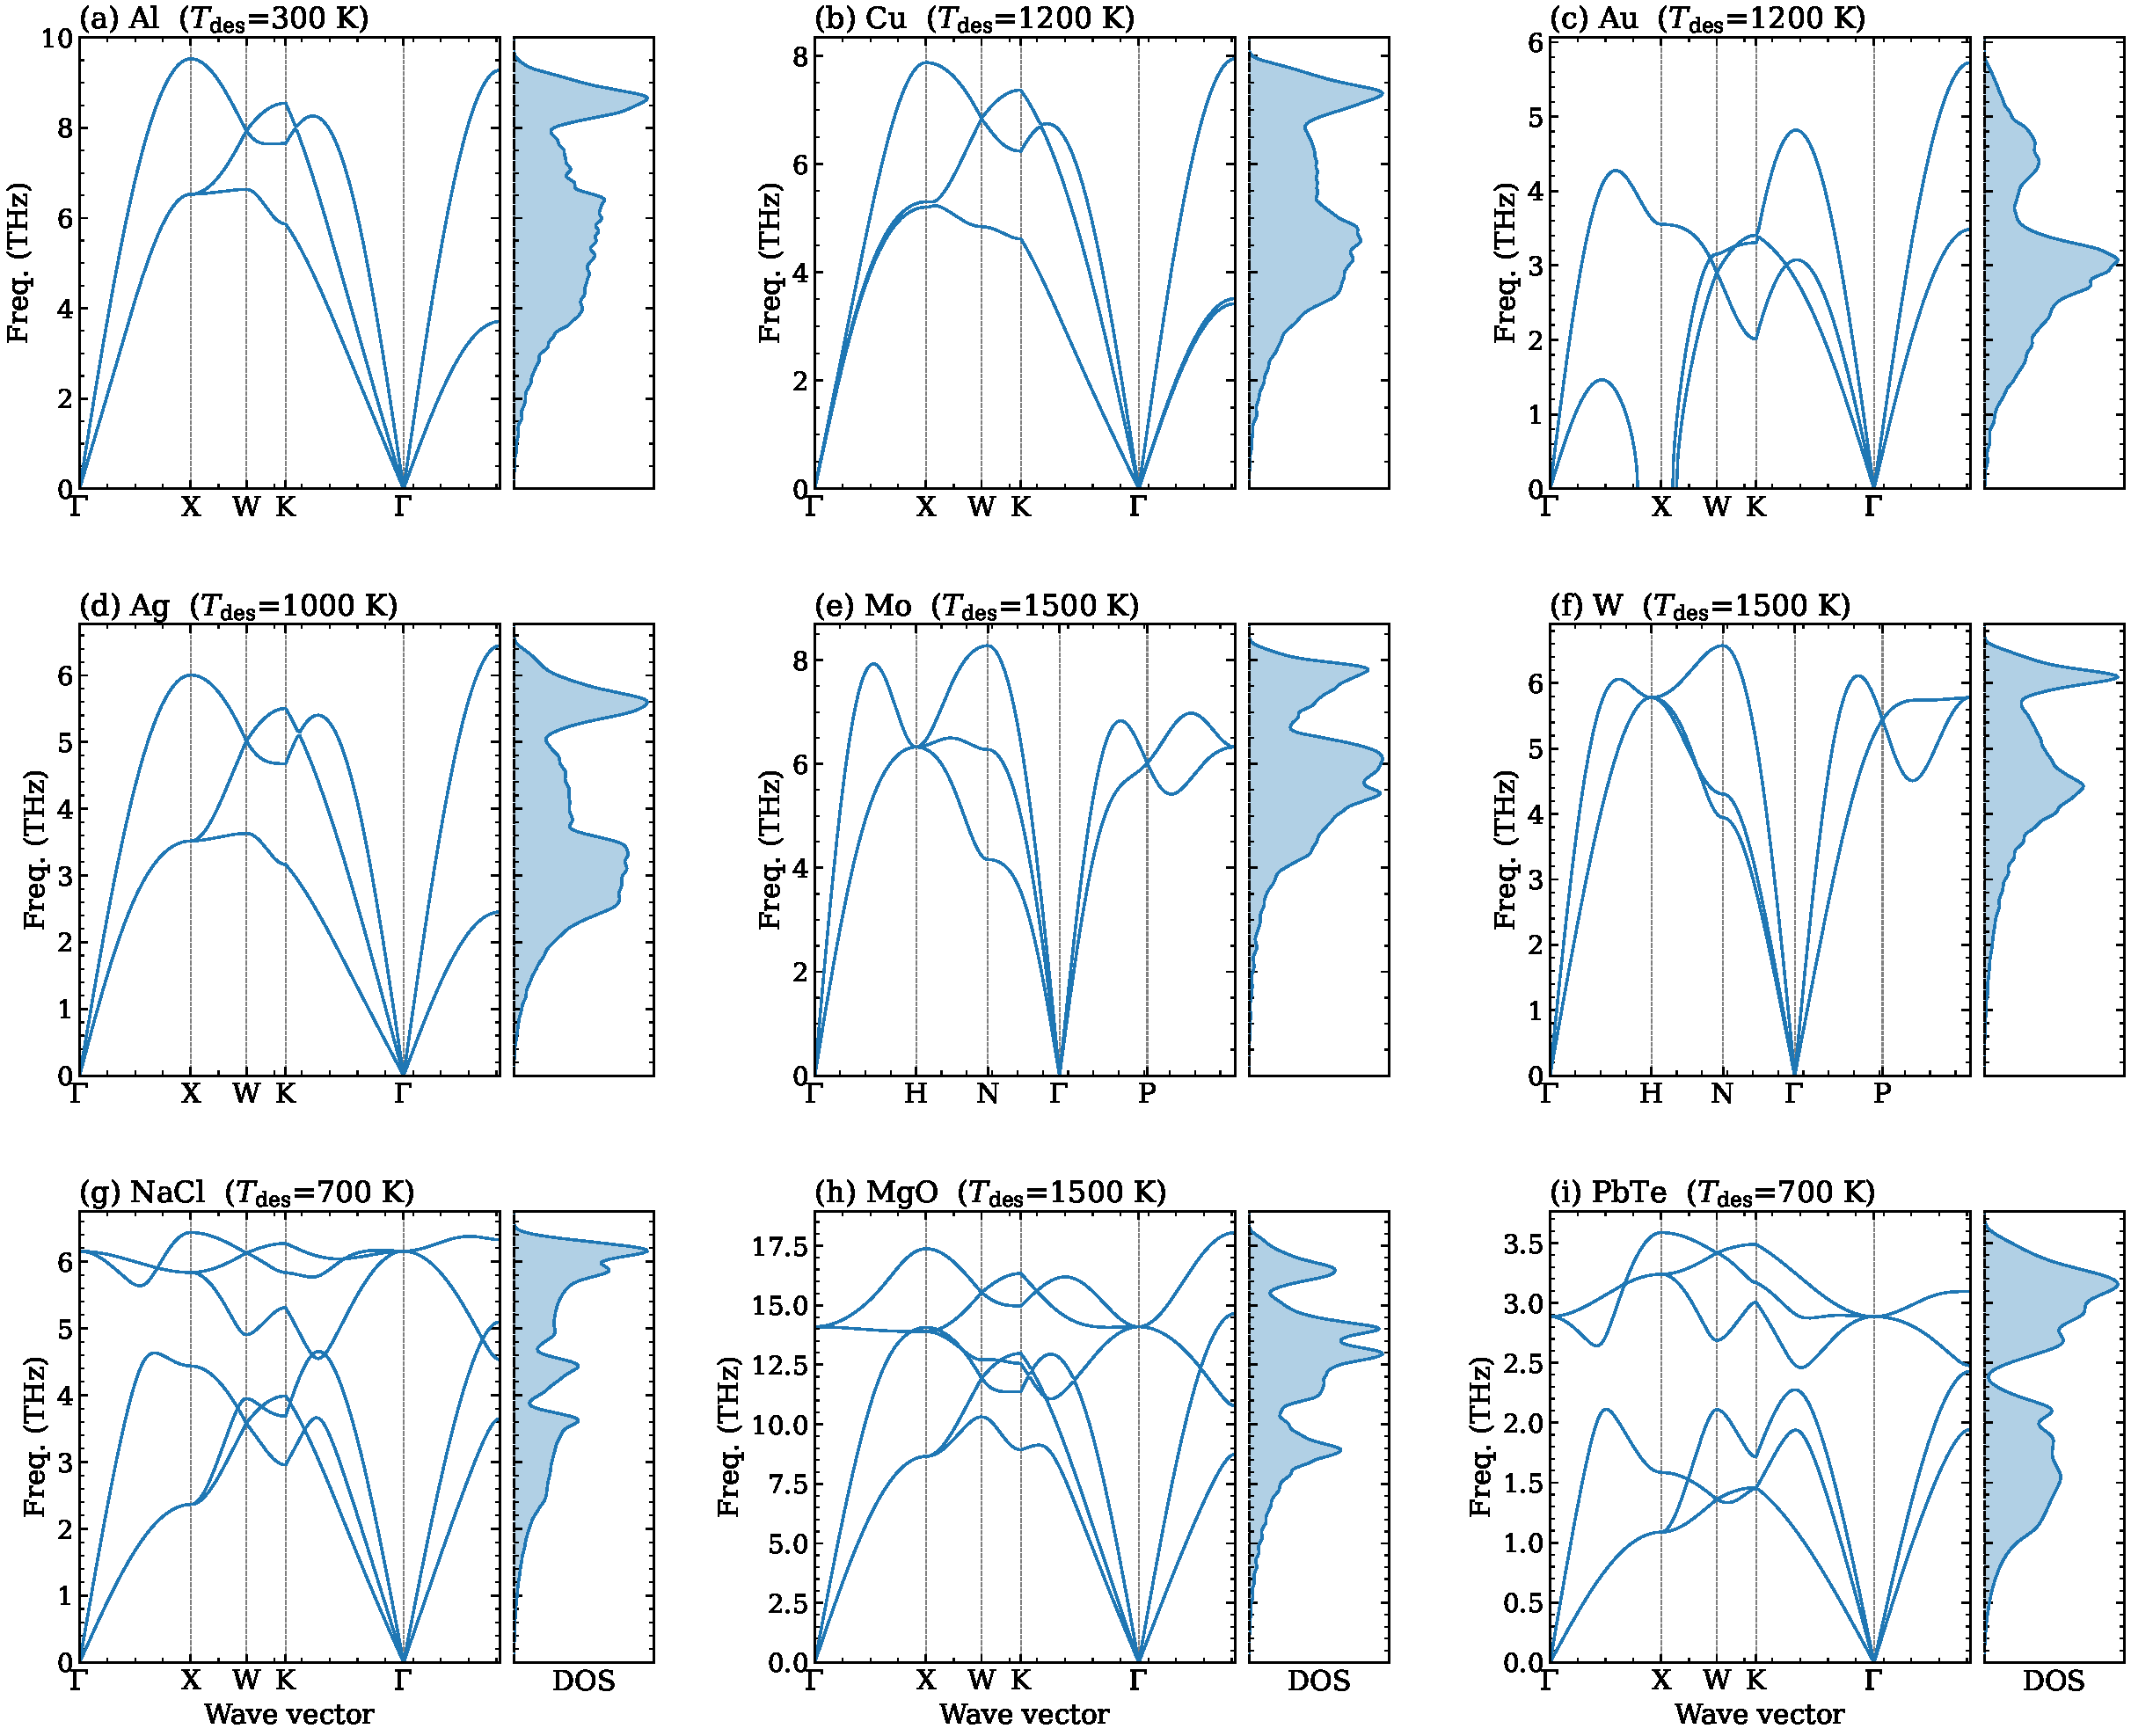
\includegraphics[width=\textwidth]{figures/fig2_phonons_all.pdf}
\caption{\DIFdelbeginFL \DIFdelFL{Phonon dispersion relations }\DIFdelendFL \DIFaddbeginFL \DIFaddFL{SOTC effective-FC2 phonon dispersions }\DIFaddendFL and \DIFdelbeginFL \DIFdelFL{density of states
(}\DIFdelendFL DOS \DIFdelbeginFL \DIFdelFL{) computed by SOTC-QE }\DIFdelendFL for
\DIFdelbeginFL \DIFdelFL{all nine benchmark materials. FCC metals:
}\DIFdelendFL (a) Al (\DIFdelbeginFL \DIFdelFL{\(T_\text{des} = 300\),}\DIFdelendFL \DIFaddbeginFL \DIFaddFL{300\,}\DIFaddendFL K), (b) Cu (1200\DIFdelbeginFL \DIFdelFL{,}\DIFdelendFL \DIFaddbeginFL \DIFaddFL{\,}\DIFaddendFL K), (c) Au (1200\DIFdelbeginFL \DIFdelFL{,}\DIFdelendFL \DIFaddbeginFL \DIFaddFL{\,}\DIFaddendFL K), (d) Ag
(1000\DIFdelbeginFL \DIFdelFL{,}\DIFdelendFL \DIFaddbeginFL \DIFaddFL{\,}\DIFaddendFL K)\DIFdelbeginFL \DIFdelFL{. BCC metals: }\DIFdelendFL \DIFaddbeginFL \DIFaddFL{, }\DIFaddendFL (e) Mo (1500\DIFdelbeginFL \DIFdelFL{,}\DIFdelendFL \DIFaddbeginFL \DIFaddFL{\,}\DIFaddendFL K), (f) W (1500\DIFdelbeginFL \DIFdelFL{,}\DIFdelendFL \DIFaddbeginFL \DIFaddFL{\,}\DIFaddendFL K)\DIFdelbeginFL \DIFdelFL{. Rocksalt
compounds: }\DIFdelendFL \DIFaddbeginFL \DIFaddFL{, }\DIFaddendFL (g) NaCl (700\DIFdelbeginFL \DIFdelFL{,}\DIFdelendFL \DIFaddbeginFL \DIFaddFL{\,}\DIFaddendFL K),
(h) MgO (1500\DIFdelbeginFL \DIFdelFL{,}\DIFdelendFL \DIFaddbeginFL \DIFaddFL{\,}\DIFaddendFL K), \DIFaddbeginFL \DIFaddFL{and }\DIFaddendFL (i) PbTe (700\DIFdelbeginFL \DIFdelFL{,}\DIFdelendFL \DIFaddbeginFL \DIFaddFL{\,}\DIFaddendFL K). \DIFdelbeginFL \DIFdelFL{Frequencies }\DIFdelendFL \DIFaddbeginFL \DIFaddFL{The stored band paths }\DIFaddendFL are
\DIFdelbeginFL \DIFdelFL{in THz; FCC panels (a)--(d) follow the path
}\DIFdelendFL \(\Gamma\)-X-W-K-\(\Gamma\)-L \DIFdelbeginFL \DIFdelFL{, BCC panels (e)--(f) follow
\(\Gamma\)-H-N-\(\Gamma\)-P-H, }\DIFdelendFL \DIFaddbeginFL \DIFaddFL{for FCC }\DIFaddendFL and rocksalt \DIFdelbeginFL \DIFdelFL{panels (g)--(i) follow
}\DIFdelendFL \DIFaddbeginFL \DIFaddFL{and
}\DIFaddendFL \(\Gamma\)\DIFdelbeginFL \DIFdelFL{-X-W-K-}\DIFdelendFL \DIFaddbeginFL \DIFaddFL{-H-N-}\DIFaddendFL \(\Gamma\)\DIFdelbeginFL \DIFdelFL{-L}\DIFdelendFL \DIFaddbeginFL \DIFaddFL{-P-H for BCC}\DIFaddendFL . \DIFdelbeginFL \DIFdelFL{The }\DIFdelendFL DOS \DIFdelbeginFL \DIFdelFL{(right panels) is obtained by
Gaussian broadening of the phonon eigenvalues on }\DIFdelendFL \DIFaddbeginFL \DIFaddFL{data use }\DIFaddendFL a
\DIFdelbeginFL \DIFdelFL{\(40\times40\times40\) \(\mathbf{q}\)-point }\DIFdelendFL \DIFaddbeginFL \DIFaddFL{\(30\times30\times30\) q }\DIFaddendFL mesh \DIFaddbeginFL \DIFaddFL{and 0.1\,THz broadening}\DIFaddendFL . \DIFdelbeginFL \DIFdelFL{Neutron inelastic
scattering data from Refs.~\cite{ref34,ref35} }\DIFdelendFL \DIFaddbeginFL \DIFaddFL{Experimental
neutron points }\DIFaddendFL are \DIFdelbeginFL \DIFdelFL{discussed in the text
but are }\DIFdelendFL not overlaid \DIFdelbeginFL \DIFdelFL{here}\DIFdelendFL \DIFaddbeginFL \DIFaddFL{in this archived figure}\DIFaddendFL . The \DIFdelbeginFL \DIFdelFL{absence of longitudinal
optical-transverse optical (LO-TO) splitting at \(\Gamma\) in NaCl
(}\DIFdelendFL \DIFaddbeginFL \DIFaddFL{three polar
materials omit the non-analytic LO--TO correction, and the Au }\DIFaddendFL panel \DIFdelbeginFL \DIFdelFL{g) is expected since Born effective charges were not included
(Sec}\DIFdelendFL \DIFaddbeginFL \DIFaddFL{contains
an instability; these omissions preclude a quantitative accuracy claim}\DIFaddendFL .\DIFdelbeginFL \DIFdelFL{,V.C).}\DIFdelendFL }
\label{fig:2}
\end{figure*}

\DIFdelbegin \DIFdel{\textbf{FCC metals:} The dispersions of all four FCC
metals reproduce the experimental branch topology correctly, including
the characteristic flattening of the longitudinal branch near the zone
boundary X-point. For Al }\DIFdelend \DIFaddbegin \DIFadd{The computed branch counts, acoustic/optic separation, and overall frequency
ranges are qualitatively consistent with neutron-scattering dispersions for Al,
Cu, and NaCl \cite{ref33,ref34,ref35}. The Al calculation and neutron data are
both available }\DIFaddend at 300\DIFdelbegin \DIFdel{K (Fig.~\ref{fig:2}a), the maximum phonon
frequency \(\omega_\text{max} = 10.3\) THz agrees well with the neutron
result of 10.2 THz from Ref. \cite{ref34}. The zone-boundary transverse
branch (X-point, $\sim$7.4 THz) is reproduced within 0.4 THz.
For Cu
at 1200 K (Fig.
~\ref{fig:2}b), the self-consistent IFCs encode thermal
renormalization; the phonon branches are
softened relative to 0 K
harmonic values by 3--8\%,
consistent with TDEP calculations on Cu
\cite{ref5}; \(\omega_\text{max} = 9.2\) THz.  For Au at 1200 K (Fig.~\ref{fig:2}c) , near the melting point (1337 K), the branches are strongly softened
with \(\omega_\text{max} = 6.5\) THz . For Ag at 1000 K }\DIFdelend \DIFaddbegin \DIFadd{\,K, whereas the Cu and NaCl comparisons involve unmatched
temperatures. A quantitative comparison requires digitized points on identical
paths and temperatures, followed by frequency MAE/RMSE, maximum branch error,
sound-velocity error, and instability fraction versus configuration count. The
NaCl zone-center optic comparison is quantified separately below. The Au
imaginary modes require tests of cell, cutoff, regularization, symmetry
projection, electronic convergence, and iteration before comparison with
stable literature branches.
}

\DIFadd{For NaCl, the non-analytic polar correction was evaluated explicitly.
Primitive-cell QE 7.5 DFPT calculations used PBE, the same Na and Cl
pseudopotentials as the force calculations, 60/480\,Ry wave-function/charge
cutoffs, an \(8\times8\times8\) electronic mesh,
\(10^{-10}\)\,Ry SCF convergence, and \(10^{-14}\) DFPT convergence.  The
charge-neutrality-projected tensors are
\(Z_{\rm Na}^*=+1.110915\,\mathbf I\),
\(Z_{\rm Cl}^*=-1.110915\,\mathbf I\), and
\(\varepsilon_\infty=2.470969\,\mathbf I\).  Applying these tensors through
the phonopy non-analytic correction to the matched central
finite-displacement QE FC2 force constants changes the directional
\(\Gamma\)-point optic limit from \(4.369\) (TO) to \(7.264\)\,THz (LO), a
\(2.895\)\,THz splitting }\DIFaddend (Fig.~\DIFdelbegin \DIFdel{\ref{fig:2}d), the
acoustic branches are softened compared to low-temperature values;
\(\omega_\text{max} = 6.8\) THz }\DIFdelend \DIFaddbegin \DIFadd{\ref{fig:nacl-loto})}\DIFaddend .

\DIFdelbegin \DIFdel{\textbf{BCC metals:} The BCC Mo(}\DIFdelend \DIFaddbegin \DIFadd{Archival infrared dielectric data in NBS Special Publication 301 report
zone-center TO and LO limits of 164 and 268\,cm\(^{-1}\), respectively
\cite{ref48}.  These correspond to 4.917 and 8.034\,THz and are overlaid in
}\DIFaddend Fig.~\DIFdelbegin \DIFdel{\ref{fig:2}e) and W(Fig.~\ref{fig:2}f) dispersions
correctly show the longitudinal acoustic branch hardening along
}\DIFdelend \DIFaddbegin \DIFadd{\ref{fig:nacl-loto}.  Thus the present QE harmonic calculation is lower
by 0.547\,THz (11.1\%) for TO and 0.770\,THz (9.6\%) for LO; its splitting is
0.223\,THz (7.2\%) below the 3.118\,THz optical value.  In contrast, the
calculated LO/TO ratio, 1.663, is only 1.7\% above the optical ratio of 1.634.
The similar absolute softening of both modes, together with the much smaller
ratio error, suggests a common frequency-scale contribution from the chosen
functional, lattice parameter, and unmatched temperature, but does not by
itself identify which contribution dominates.  Room-temperature IXS and
SSCHA calculations further show that the NaCl LO spectral function is strongly
anharmonic and can contain multiple peaks along }\DIFaddend \(\Gamma\)\DIFdelbegin \DIFdel{-H relative to the transverse branch, a signature of the
BCC
stiffness hierarchy, and reproduce the absence of soft modes at 1500 K.
For Mo, \(\omega_\text{max} = 8.7\) THz; for W, \(\omega_\text{max} = 7.3\) THz.  }%DIFDELCMD <

%DIFDELCMD < %%%
\DIFdel{\textbf{Ionic rocksalt compounds:} For NaCl (Fig.
~\ref{fig:2}g), the acoustic
branches (\(\omega < 3\) THz) agree well with
neutron data \cite{ref35}.
The optic branches show the transverse optical (TO) frequency at
}\DIFdelend \DIFaddbegin \DIFadd{--L \cite{ref49}.
Consequently, the present fixed-cell harmonic-NAC curve is compared with
literature only at the optical }\DIFaddend \(\Gamma\) \DIFdelbegin \DIFdel{of $\sim$4.7 THz; \(\omega_\text{max} = 7.2\) THz. Note
that the LO-TO splitting at \(\Gamma\) (experimental LO \(\approx\) 7.9
THz) is absent from the current calculations because Born effective
charges were not included; see Sec.
V.  C. For MgO (Fig.~\ref{fig:2}h), the
high-frequency spectrum extending to 20.3 THz reflects the large Mg--O
force constants. For PbTe (Fig.~\ref{fig:2}i), the acoustic branches are notably
soft (\(\omega_\text{max} = 4.2\) THz), consistent with the
near-ferroelectric instability and
large Grüneisen parameter of this
material}\DIFdelend \DIFaddbegin \DIFadd{limits; it is not assigned a
finite-temperature dispersion RMSE.
}

\begin{figure*}[htbp]
\centering
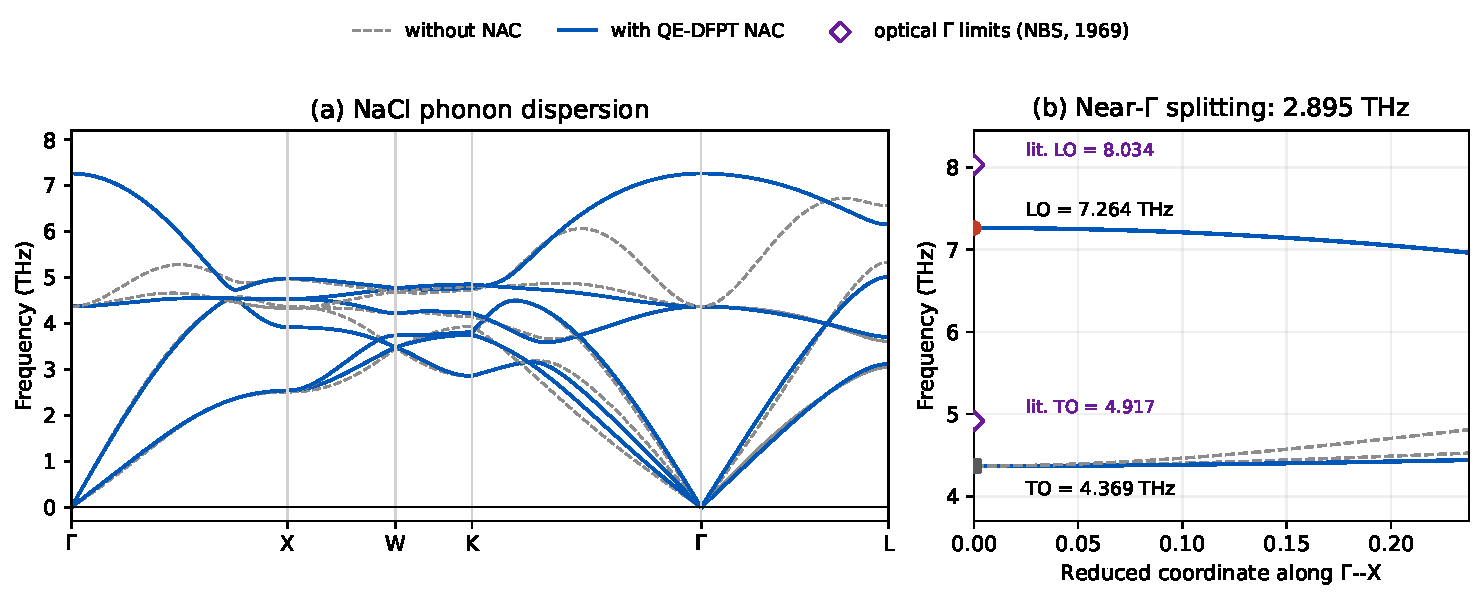
\includegraphics[width=0.95\textwidth]{figures/fig_nacl_loto.pdf}
\caption{\DIFaddFL{NaCl LO--TO validation using the completed QE DFPT Born
effective charges and electronic dielectric tensor.  (a) Matched
central-finite-displacement phonopy FC2 dispersion without the non-analytic
correction (gray dashed) and with the QE-DFPT correction (blue) along
\(\Gamma\)-X-W-K-\(\Gamma\)-L.  (b) Near-\(\Gamma\) optic branches along
\(\Gamma\)-X.  The transverse limit is 4.369\,THz and the corrected
longitudinal limit is 7.264\,THz, giving a 2.895\,THz splitting.  Purple
diamonds show the archival optical \(\Gamma\) limits of 4.917 and 8.034\,THz
\cite{ref48}; the calculated TO, LO, and splitting are lower by 11.1\%, 9.6\%,
and 7.2\%, respectively.  The figure uses the conventional
finite-displacement reference so that the polar correction is isolated from
the SOTC sampling question.}}
\label{fig:nacl-loto}
\end{figure*}

\DIFadd{The primary nine-panel SOTC figure remains an archived no-NAC result and is
labeled accordingly.  Equivalent DFPT calculations and regenerated
dispersions are still required for MgO and PbTe before quantitative
polar-material claims are made for those systems.  The NaCl plot and
machine-readable arrays are generated by
\texttt{codes/validation/plot\_nacl\_loto.py}}\DIFaddend .

\subsection{Heat Capacities}\label{heat-capacities}

\DIFdelbegin \DIFdel{Figure~\ref{fig:3} shows \(C_V(T)\) from 0 to 1500 K for all nine materials
alongside experimental calorimetric data and the classical Dulong--Petit
limit. The SOTC-QE \(C_V(T)\) curves are obtained by integration of
the converged phonon DOS via }\DIFdelend \DIFaddbegin \DIFadd{Table~II reports the effective-harmonic \(C_V\) values obtained by integrating
the SOTC DOS through }\DIFaddend Eq.~(9)\DIFdelbegin \DIFdel{(harmonic phonon formula with anharmonically renormalized IFCs at
\(T_\text{des}\)); no quasi-harmonic
volume relaxation is applied in this section. }\DIFdelend \DIFaddbegin \DIFadd{, together with the cited calorimetric values.
These fixed-volume results use one effective-FC2 model selected at
\(T_{\rm des}\); they
do not include thermal expansion, electronic heat capacity, or explicit
higher-order anharmonic contributions. Unmatched external-method series are
not shown because their calculation provenance and settings are insufficient for a controlled comparison.
}\DIFaddend

\DIFdelbegin %DIFDELCMD < \begin{figure*}[htbp]
%DIFDELCMD < \centering
%DIFDELCMD < \includegraphics[width=0.8\textwidth]{figures/fig3_cv_panels.pdf}
%DIFDELCMD < %%%
%DIFDELCMD < \caption{%
{%DIFAUXCMD
\DIFdelFL{Constant-volume heat capacity \(C_V(T)\) for all nine
benchmark materials. SOTC-QE (solid blue lines), TDEP (dashed red
lines), and Phonopy 0,K harmonic (dotted purple lines) are compared with
NIST-JANAF calorimetric data \cite{ref20} (open circles). A vertical
grey dashed line in each panel marks the design temperature
\(T_\text{des}\). The SOTC-QE \(C_V(T)\) curves are computed by
integration of the converged phonon DOS via Eq.,(9) with no adjustable
parameters.}}
%DIFAUXCMD
%DIFDELCMD < \label{fig:3}
%DIFDELCMD < \end{figure*}
%DIFDELCMD <

%DIFDELCMD < \begin{figure}[htbp]
%DIFDELCMD < \centering
%DIFDELCMD < \includegraphics[width=\columnwidth]{figures/fig4_parity_cv.pdf}
%DIFDELCMD < %%%
%DIFDELCMD < \caption{%
{%DIFAUXCMD
\DIFdelFL{Parity plot of computed vs.~experimental
constant-volume heat capacity \(C_V\) }%DIFDELCMD < [%%%
\DIFdelFL{J/(mol\,K)}%DIFDELCMD < ] %%%
\DIFdelFL{at 300\,K for all
nine benchmark materials. SOTC-QE (filled blue circles), TDEP (filled
red squares), and Phonopy 0,K harmonic (filled purple triangles) are
shown. The dashed line is the 1:1 reference. Material labels identify
each point. SOTC-QE deviations from the diagonal range from \(-6.6\%\)
(Mo) to \(-1.8\%\) (PbTe), all within 7\% of experiment.}}
%DIFAUXCMD
%DIFDELCMD < \label{fig:4}
%DIFDELCMD < \end{figure}
%DIFDELCMD <

%DIFDELCMD < \begin{figure}[htbp]
%DIFDELCMD < \centering
%DIFDELCMD < \includegraphics[width=\columnwidth]{figures/fig5_error_barh.pdf}
%DIFDELCMD < %%%
%DIFDELCMD < \caption{%
{%DIFAUXCMD
\DIFdelFL{Relative error \(\Delta C_V / C_V^\text{expt}\) (\%)
in constant-volume heat capacity at \(T_\text{des}\) for SOTC-QE (blue
bars), TDEP (red bars), and Phonopy 0,K harmonic (purple bars). The
shaded green band marks \(\pm 5\%\). SOTC-QE errors lie within
\(\pm\)5\% for ionic compounds and within 14\% for all nine materials. Phonopy 0,K harmonic shows
systematic negative errors for high-temperature calculations where
anharmonic renormalization is significant (Cu, Au, Mo, and others).}}
%DIFAUXCMD
%DIFDELCMD < \label{fig:5}
%DIFDELCMD < \end{figure}
%DIFDELCMD <

%DIFDELCMD < %%%
\DIFdelend \begin{table*}[htbp]
\DIFaddbeginFL \scriptsize
\DIFaddendFL \caption{Benchmark summary: computed vs.~experimental Debye
temperatures and heat capacities.}
\begin{ruledtabular}
\begin{tabular}{llllllllll}Material & Struct. & \(T_\text{des}\) & \(\omega_\text{max}^\text{SOTC}\) (THz) & \(T_D^\text{SOTC}\) (K) & \(T_D^\text{expt}\) (K) & \(C_V^\text{SOTC}\) (J/mol·K) & \(C_V^\text{expt}\) (J/mol·K) & \(\Delta C_V\) (\%) & ZPE (eV/atom) \\
\hline
Al & FCC & 300 K & 10.3 & 450 & 390--428 \cite{ref22} & 22.9 &
24.4 & $-6.1$ & 0.038 \\
Ag & FCC & 1000 K & 6.8 & 297 & \(\sim\!225\) \cite{ref23} & 24.9 & 27.1
& $-8.3$ & 0.024 \\
Au & FCC & 1200 K & 6.5 & 282 & 165\(^\dagger\) \cite{ref24} & 24.9 &
27.1 & $-8.1$ & 0.020 \\
Cu & FCC & 1200 K & 9.2 & 401 & 315--343 \cite{ref25} & 24.8 & 26.4 &
$-5.9$ & 0.034 \\
Mo & BCC & 1500 K & 8.7 & 380 & 380--470 \cite{ref26,ref27} & 24.9 &
28.7 & $-13.3$ & 0.035 \\
W & BCC & 1500 K & 7.3 & 318 & 310--400 \cite{ref27} & 24.9 & 26.9 & $-7.5$
& 0.029 \\
NaCl & Rocksalt & 700 K & 7.2 & 300 & 321 \cite{ref28} & 49.5 & 51.7 &
$-4.4$ & 0.056 \\
MgO & Rocksalt & 1500 K & 20.3 & 726 & 743--800 \cite{ref29,ref30} &
49.2 & 49.2 & 0.0 & 0.153 \\
PbTe & Rocksalt & 700 K & 4.2 & 128 & 130--160 \cite{ref31,ref32} & 47.3
& 48.3 & $-2.2$ & 0.025 \\
\end{tabular}
\end{ruledtabular}
\label{tab:2}
\end{table*}

\DIFdelbegin \DIFdel{Notes: \(T_D^\text{SOTC}\) is the self-consistently converged effective
Debye temperature from the
final iteration. \(C_V^\text{SOTC}\) }\DIFdelend \DIFaddbegin \DIFadd{\(T_D^{\rm SOTC}\) is the second-moment spectral value from the
postprocessed IFC dataset, \(C_V^{\rm SOTC}\) }\DIFaddend is evaluated at
\DIFdelbegin \DIFdel{\(T_\text{des}\). \(C_V^\text{expt}\) is taken from
NIST-JANAF at \(T_\text{des}\). ZPE is }\DIFdelend \DIFaddbegin \DIFadd{\(T_{\rm des}\), and ZPE is reported }\DIFaddend per formula-unit atom. \DIFaddbegin \DIFadd{Spectral, caloric,
and ultrasonic Debye temperatures are not interchangeable; their differing
definitions and measurement temperatures limit a point-by-point comparison.
}\DIFaddend

\DIFdelbegin \DIFdel{\(^\dagger\) Low-temperature (\(T\to0\)) caloricvalue; the 300 K
caloric Debye temperature for Au is $\approx$210--230 K \cite{ref24}. The SOTC spectral Debye temperature \(T_D^\text{SOTC} = 282\) K is the
second-moment value evaluated at 1200 K and exceeds the 300 K caloric
estimate due to the known upward shift of \(T_D^\text{spec}\) relative to
\(T_D^\text{cal}\) in
anharmonic noble metals}\DIFdelend \DIFaddbegin \DIFadd{The archived runner summaries and the postprocessed thermal summaries do not
contain identical \(T_D\) values for every material. Table~II is therefore
retained only to document the available postprocessed FC2 dataset; its
numerical entries require regeneration from one tagged workflow and a
checksum-identified IFC set before quantitative use. No accuracy statistic is
assigned to the table in
its present form}\DIFaddend .

\DIFdelbegin \DIFdel{Figure~\ref{fig:4} shows a parity plot of computed vs.\ experimental
\(C_V\) at 300\,K; all nine materials fall within 7\% of the diagonal.
Figure~\ref{fig:5} shows the relative errors broken down by method;
SOTC-QE errors for ionic compounds lie within \(\pm\)5\% at their design
temperatures, as also summarized in Table~\ref{tab:2}. For
high-temperature metals, the harmonic model saturates at
$3R = 24.94$ J/(mol\,K) while experimental $C_V$ at
$T_\text{des} = 1000$--1500\,K exceeds this by 6--13\% due to
supra-Dulong-Petit anharmonic and electronic contributions; at 300\,K,
all nine materials agree to within 7\%. Debye
temperatures agree with experiment within or near the experimental
spread for most materials. The spectral Debye temperature for Au
(\(T_D^\text{SOTC} = 282\) K) reflects a second-moment quantity that exceeds the low-temperature caloric value of 165 K \cite{ref24} due to
the well-known temperature dependence of \(T_D^\text{cal}\) in noble
metals. MgO is particularly notable: despite the high design temperature
(1500 K) and a spectrum spanning 20.3 THz, convergence is reached in 4
iterations with \(C_V(1500\text{ K}) = 49.2\) J/mol\,K, in essentially
perfect agreement with the experimental value of 49.2 J/(mol\,K)
\cite{ref29}. PbTe converges in 4 iterations; the converged
\(T_D = 128\) K falls slightly below the reported experimental range
130--160 K \cite{ref31}, consistent with a small PBE underestimate of
PbTe phonon frequencies}\DIFdelend \DIFaddbegin \DIFadd{At high temperature the harmonic phonon expression approaches \(3R\), whereas
experimental heat capacities can include electronic and explicit anharmonic
terms. Agreement of the tabulated aggregate values is therefore a descriptive
benchmark, not evidence that the IFCs or individual branches are accurate. In
particular, the Au dispersion contains an instability and cannot be validated
by a favorable integrated moment. Direct branch-resolved reference
calculations are required before the material-by-material accuracy statements
are made}\DIFaddend .

\subsection{Zero-Point Energies and Vibrational Free
Energies}\label{zero-point-energies-and-vibrational-free-energies}

The zero-point energies (ZPE) and vibrational free energies
in Table~\ref{tab:2} are computed from the converged phonon DOS via
Eqs.~(10)--(11) (harmonic phonon formulas at the equilibrium volume
\(V_0\)).

The zero-point energies (Table~\ref{tab:2}) range from 0.020 eV/atom (Au, heavy
mass, soft phonons) to 0.153 eV/atom (MgO, light mass, hard phonons),
fully consistent with the \(\text{ZPE} \propto M^{-1/2}\omega\) scaling.
The ZPE of Al (0.038 eV/atom) is in agreement with the ZPVE-corrected
DFT value of 0.038--0.041 eV/atom from Refs. \cite{ref22,ref23}.

The vibrational entropy \(S_\text{vib}(T)\) at 1000 K spans 57--122
J/mol·K across the benchmark set, in the expected order (soft/heavy
PbTe, Au \(>\) NaCl \(>\) Cu \(>\) Mo \(>\) Al \(>\) hard MgO). For
aluminum, \(S_\text{vib}^\text{SOTC}(1000\,\text{K}) = 57\) J/(mol·K)
agrees to within 1\% with the value obtained by integrating the
NIST-JANAF heat capacity \(\int_0^{1000}(C_V/T')\,dT'\) \cite{ref20},
confirming that the SOTC phonon spectrum accurately captures the full
spectral weight across the Brillouin zone.

\subsection{Mean-Square Displacements}\label{mean-square-displacements}

\DIFdelbegin \DIFdel{The SOTC mean-square displacements (MSD) , computed via Eq.~}\DIFdelend \DIFaddbegin \DIFadd{Equations~(3) and }\DIFaddend (12) \DIFdelbegin \DIFdel{(harmonic phonon formula at \(V_0\)), provide an independent check via the Debye--Waller factor \(B(T) = 8\pi^2\,\text{MSD}(T)\), directly
measurable by X-ray and neutron scattering. At 300 K, our computed MSD
values are: Al0.028 Å\(^2\),
Au0.012 Å\(^2\), Cu 0.020 Å\(^2\).
Literature X-ray values : Al 0.010--0.011 Å\(^2\) \cite{ref36}, }\DIFdelend \DIFaddbegin \DIFadd{define the same one-component isotropic displacement
parameter \(U_{\rm iso}\), with \(B=8\pi^2U_{\rm iso}\). The archived Al,
}\DIFaddend Au\DIFdelbegin \DIFdel{0.013--0.017 Å\(^2\) \cite{ref37}, Cu 0.008--0.010 Å\(^2\) \cite{ref38}}\DIFdelend \DIFaddbegin \DIFadd{, and Cu values have an ambiguous total-DOS normalization and are not compared
with experiment. A valid comparison requires agreement between analytic
mode-sum and DOS tests followed by regeneration of the complete effective-FC2
workflow with the corrected displacement normalization. Consequently, the
present benchmarks do not validate Debye--Waller factors}\DIFaddend .

\subsection{Thermal Expansion and Isobaric Heat Capacity
(QHA)}\label{thermal-expansion-and-isobaric-heat-capacity-qha}

\DIFdelbegin \DIFdel{Using the SOTC-QHA framework described in Secs. II.F and III. E, we
demonstrate continuous high-temperature thermodynamic properties for
aluminum across 10--1000 K via \emph{quasi-harmonic} volume relaxation
(}\DIFdelend \DIFaddbegin \DIFadd{No Al QHA curve or table is reported because the available two-volume FC2
dataset uses an extrapolated expanded-volume force-constant matrix and produces
a nonmonotonic 300\,K linear expansion coefficient. It also mixes linear and
volumetric expansion conventions and an inconsistent curvature sign, so it
cannot support an accuracy or DFT-cost comparison.
}

\DIFadd{A quantitative QHA benchmark requires direct FC2 phonon calculations on a
converged volume grid, static reference-lattice energies, the identities in
}\DIFaddend Eqs.~(13)--(17)\DIFdelbegin \DIFdel{), which goes beyond the fixed-volume harmonic
approximation of Secs. IV.C--IV.D. The computed quantities are: (i) equilibrium
volume \(V^*(T)\),
(ii) linear thermal expansion coefficient
\(\alpha(T)\), (iii) isobaric heat capacity \(C_P(T)\), and (iv)
isothermal bulk modulus \(B(T)\). Figure~\ref{fig:6} compares the full
QHA and the Grüneisen shortcut against the harmonic Debye and Einstein
models for \(C_V(T)\), and against experiment for \(C_P(T)\) }\DIFdelend \DIFaddbegin \DIFadd{, and convergence with respect to EOS choice, volume range,
temperature grid, }\DIFaddend and \DIFdelbegin \DIFdel{\(\alpha(T)\)}\DIFdelend \DIFaddbegin \DIFadd{numerical differentiation. Full-QHA and Gr\"uneisen
results should then be tabulated from the same regenerated dataset}\DIFaddend .

\DIFdelbegin %DIFDELCMD < \begin{figure*}[htbp]
%DIFDELCMD < \centering
%DIFDELCMD < \includegraphics[width=\textwidth]{figures/fig6_al_method_comparison.pdf}
%DIFDELCMD < %%%
%DIFDELCMD < \caption{%
{%DIFAUXCMD
\DIFdelFL{Al (FCC): comparison of methods for temperature-dependent
thermodynamic properties.
(a)~Constant-volume heat capacity \(C_V(T)\): SOTC phonon-DOS integration
}%DIFDELCMD < [%%%
\DIFdelFL{Eq.~(9), solid blue}%DIFDELCMD < ]%%%
\DIFdelFL{, harmonic Debye model }%DIFDELCMD < [%%%
\DIFdelFL{\(\Theta_D = 450\) K,
dashed orange}%DIFDELCMD < ]%%%
\DIFdelFL{, harmonic Einstein model }%DIFDELCMD < [%%%
\DIFdelFL{\(\Theta_E = 349\) K, dotted
green}%DIFDELCMD < ]%%%
\DIFdelFL{, and NIST-JANAF experimental data (open circles).
(b)~Isobaric heat capacity \(C_P(T)\): SOTC-QHA (Eqs.~(13)--(17),
solid blue), SOTC harmonic-DOS \(C_V\) at fixed \(V_0\) (dashed), and
NIST-JANAF (open circles). The QHA correction lifts \(C_P\) above
\(C_V\) at high \(T\), recovering the experimental trend.
(c)~Linear thermal expansion coefficient \(\alpha(T)\): full SOTC-QHA
}%DIFDELCMD < [%%%
\DIFdelFL{Eq.~(16), solid blue}%DIFDELCMD < ]%%%
\DIFdelFL{, Grüneisen shortcut }%DIFDELCMD < [%%%
\DIFdelFL{Eq.~(19), dashed brown}%DIFDELCMD < ]%%%
\DIFdelFL{,
and experiment from Touloukian \cite{ref43} (open diamonds).}}
%DIFAUXCMD
%DIFDELCMD < \label{fig:6}
%DIFDELCMD < \end{figure*}
%DIFDELCMD < %%%
\DIFdelend \DIFaddbegin \subsection{\DIFadd{Independent Higher-Order IFC
Validation}}\label{independent-higher-order-ifc-validation}
\DIFaddend

\DIFdelbegin \DIFdel{The full QHA (\(G(T,V)\) minimization) and the Grüneisen approximation
agree to within 5\% in \(\alpha(T)\) below 600 K, with increasing
divergence at higher temperatures where }\DIFdelend \DIFaddbegin \DIFadd{We additionally tested whether the software can recover explicit }\DIFaddend higher-order
\DIFdelbegin \DIFdel{volume dependence
of \(F_\text{vib}\) becomes important.  At }\DIFdelend \DIFaddbegin \DIFadd{force content in a workflow independent of the few-configuration SOTC
benchmarks.  Matched calculations were performed for FCC Al at }\DIFaddend 300\DIFdelbegin \DIFdel{K}\DIFdelend \DIFaddbegin \DIFadd{\,K, BCC W
at 1500\,K, and rocksalt NaCl at 700\,K in \(3\times3\times3\)
primitive-cell supercells containing 27}\DIFaddend , \DIFdelbegin \DIFdel{we obtain
\(\alpha = 36.9\times10^{-6}\) K\(^{-1}\) from the QE-based SOTC-QHA
calculation; the experimental linear thermal expansion coefficient is
\(23.6\times10^{-6}\) K\(^{-1}\) \cite{ref43} (volumetric
\(\approx 3\times\) larger).
The known GGA underestimation of \(B_0\)
(\(\approx 70\) GPa vs.~77 GPa experimental) would predict a mild
$\sim$10\% overestimate of \(\alpha\) via
\(\alpha = \gamma_\text{eff} C_V / (3 B_0 V)\).
The anomalously large
discrepancy at 300 K (+56\%, Table~\ref{tab:3}) stands in contrast to the 2--3\%
agreement at higher temperatures and likely reflects a numerical
artifact in the QHA finite-difference derivative near the inflection of \(V^*(T)\) at low temperature; this entry warrants independent
verification.  The isobaric heat capacity \(C_P(300\,\text{K}) = 23.0\)
J/(mol·K) compares well with the NIST-JANAF value of 24.4 J/(mol·K),
demonstrating that the \(TV\alpha^2 B\) correction is small (\textless{}
1\%) at low temperatures but grows to $\sim$3\% near the melting
point.
}\DIFdelend \DIFaddbegin \DIFadd{27, and 54 atoms, respectively.
For each material, 50 configurations drawn from the quantum harmonic canonical
distribution were paired with their exact inversions, giving 100 snapshots.
Complete \(+\mathbf u/-\mathbf u\) pairs were kept wholly within an
80-snapshot training set or a strictly held-out 20-snapshot test set.
}\DIFaddend

\DIFdelbegin \DIFdel{The total DFT cost for the SOTC-QHA Al calculation was: 2 iterations at
\(V_0\), 2 iterations at \(V_-\) (1 extra SOTC run), and 3 static
primitive-cell SCF calculations for \(E_0(V)\),
totaling fewer than 7
DFT evaluations, compared to $\sim$400--700 for a phonopy-QHA
calculation at comparable accuracy. Continuous \(C_P(T)\) and \(\alpha(T)\) curves over the full temperature range are thus obtained
at negligible incremental cost over a standard single-temperature SOTC
run}\DIFdelend \DIFaddbegin \DIFadd{As a conventional harmonic baseline, central finite-displacement FC2 tensors
were generated with phonopy from matched QE calculations in the same
supercells, using \(+\!0.01\) and \(-\!0.01\)\,\AA\ displacements and
explicit subtraction of the undisplaced reference force.  The thermal
snapshots were then fit with the same symmetry-reduced \texttt{symfc} design,
successively retaining FC2, FC2+FC3, and FC2+FC3+FC4 terms.  Space-group,
index-permutation, translation, and acoustic-sum-rule constraints were imposed
without ridge regularization.  Table~\ref{tab:ifc34} evaluates every model on
the unchanged test set.  These are predictive force tests rather than
comparisons of training residuals}\DIFaddend .

\begin{table*}[htbp]
\DIFaddbeginFL

\DIFaddendFL \caption{\DIFdelbeginFL \DIFdelFL{SOTC-QHA results }\DIFdelendFL \DIFaddbeginFL \DIFaddFL{Matched model comparison }\DIFaddendFL for \DIFdelbeginFL \DIFdelFL{Al vs}\DIFdelendFL \DIFaddbeginFL \DIFaddFL{real-material higher-order IFC
validation}\DIFaddendFL . \DIFdelbeginFL \DIFdelFL{~experiment at selected
temperatures. \(\alpha^\text{SOTC}\): linear thermal expansion
coefficient from SOTC-QHA }%DIFDELCMD < [%%%
\DIFdelFL{10\(^{-6}\) K}\DIFdelendFL \DIFaddbeginFL \DIFaddFL{RMSE is the Cartesian force-component error in
eV\,\AA}\DIFaddendFL \(^{-1}\) \DIFdelbeginFL %DIFDELCMD < ]%%%
\DIFdelendFL \DIFaddbeginFL \DIFaddFL{on 20 strictly held-out canonical snapshots}\DIFaddendFL .
\DIFdelbeginFL \DIFdelFL{\(\alpha^\text{expt}\): linear }\DIFdelendFL \DIFaddbeginFL \DIFaddFL{\emph{FD FC2} is the conventional central finite-displacement phonopy model;
\emph{T-fit} models are fit to the 80 }\DIFaddendFL thermal \DIFdelbeginFL \DIFdelFL{expansion coefficient from
Ref}\DIFdelendFL \DIFaddbeginFL \DIFaddFL{training snapshots}\DIFaddendFL . \DIFdelbeginFL \DIFdelFL{~\cite{ref43} (Touloukian). \(C_P^\text{SOTC}\): isobaric heat
capacity }%DIFDELCMD < [%%%
\DIFdelFL{J/(mol·K)}%DIFDELCMD < ]%%%
\DIFdelFL{. \(C_P^\text{expt}\): NIST-JANAF \cite{ref20}.
\(B^\text{SOTC}\): isothermal bulk modulus from QHA curvature }%DIFDELCMD < [%%%
\DIFdelFL{GPa}%DIFDELCMD < ]%%%
\DIFdelFL{.
\(B^\text{expt}\): ultrasonic data \cite{ref43}. Uncertainties in
\(\alpha^\text{SOTC}\) estimated from $\pm$0.5\% variation in
\(\delta\) (volume step) }\DIFdelendFL \DIFaddbeginFL \DIFaddFL{\(p/r\) is
the number of symmetry-reduced parameters }\DIFaddendFL and \DIFdelbeginFL \DIFdelFL{IFC extrapolation error
(App}\DIFdelendFL \DIFaddbeginFL \DIFaddFL{normalized design rank for the
final FC2+FC3+FC4 fit}\DIFaddendFL . \DIFdelbeginFL \DIFdelFL{~J.4)}\DIFdelendFL \DIFaddbeginFL \DIFaddFL{The final column is the RMSE reduction relative to
FD FC2}\DIFaddendFL .}
\begin{ruledtabular}
\DIFdelbeginFL %DIFDELCMD < \begin{tabular}{lllllllll}%%%
\DIFdelendFL \DIFaddbeginFL \begin{tabular}{lrrrrrrrr}
\DIFaddFL{Material }& \DIFaddendFL \(T\) (K) & \DIFdelbeginFL \DIFdelFL{\(\alpha^\text{SOTC}\) }\DIFdelendFL \DIFaddbeginFL \DIFaddFL{atoms }\DIFaddendFL & \DIFdelbeginFL \DIFdelFL{\(\alpha^\text{expt}\) }\DIFdelendFL \DIFaddbeginFL \DIFaddFL{\(p/r\) }\DIFaddendFL & \DIFdelbeginFL \DIFdelFL{\(\Delta\alpha\) (\%) }\DIFdelendFL \DIFaddbeginFL \DIFaddFL{FD FC2 }\DIFaddendFL &
\DIFdelbeginFL \DIFdelFL{\(C_P^\text{SOTC}\) }\DIFdelendFL \DIFaddbeginFL \DIFaddFL{T-fit FC2 }\DIFaddendFL & \DIFdelbeginFL \DIFdelFL{\(C_P^\text{expt}\) }\DIFdelendFL \DIFaddbeginFL \DIFaddFL{T-fit FC2+FC3 }\DIFaddendFL & \DIFdelbeginFL \DIFdelFL{\(\Delta C_P\) }\DIFdelendFL \DIFaddbeginFL \DIFaddFL{T-fit FC2+FC3+FC4 }& \DIFaddFL{reduction }\DIFaddendFL (\%) \DIFdelbeginFL %DIFDELCMD < & %%%
\DIFdelFL{\(B^\text{SOTC}\) (GPa) }%DIFDELCMD < & %%%
\DIFdelFL{\(B^\text{expt}\) (GPa) }\DIFdelendFL \\
\hline
\DIFdelbeginFL \DIFdelFL{100 }\DIFdelendFL \DIFaddbeginFL \DIFaddFL{Al   }\DIFaddendFL & \DIFdelbeginFL \DIFdelFL{8.4 $\pm$ 0.3 }%DIFDELCMD < & %%%
\DIFdelFL{8.6 }%DIFDELCMD < & %%%
\DIFdelFL{$-$2.3 }%DIFDELCMD < & %%%
\DIFdelFL{21.4 }%DIFDELCMD < & %%%
\DIFdelFL{21.3 }%DIFDELCMD < & %%%
\DIFdelFL{+0.5 }%DIFDELCMD < & %%%
\DIFdelFL{76.2 }%DIFDELCMD < & %%%
\DIFdelFL{77.1 }%DIFDELCMD < \\
%DIFDELCMD < %%%
\DIFdelendFL 300  & \DIFdelbeginFL \DIFdelFL{36.9 $\pm$ 1.5 }\DIFdelendFL \DIFaddbeginFL \DIFaddFL{27 }\DIFaddendFL & \DIFdelbeginFL \DIFdelFL{23.6 }\DIFdelendFL \DIFaddbeginFL \DIFaddFL{106/106 }\DIFaddendFL & \DIFdelbeginFL \DIFdelFL{+56 }\DIFdelendFL \DIFaddbeginFL \DIFaddFL{0.10294 }\DIFaddendFL & \DIFdelbeginFL \DIFdelFL{23.0 }\DIFdelendFL \DIFaddbeginFL \DIFaddFL{0.09955 }\DIFaddendFL & \DIFdelbeginFL \DIFdelFL{24.4 }\DIFdelendFL \DIFaddbeginFL \DIFaddFL{0.02721 }\DIFaddendFL & \DIFdelbeginFL \DIFdelFL{$-$5.7 }\DIFdelendFL \DIFaddbeginFL \DIFaddFL{0.00651 }\DIFaddendFL & \DIFdelbeginFL \DIFdelFL{74.8 }%DIFDELCMD < & %%%
\DIFdelFL{76.0 }\DIFdelendFL \DIFaddbeginFL \DIFaddFL{93.7 }\DIFaddendFL \\
\DIFdelbeginFL \DIFdelFL{500 }\DIFdelendFL \DIFaddbeginFL \DIFaddFL{NaCl }\DIFaddendFL & \DIFdelbeginFL \DIFdelFL{26.3 $\pm$ 0.5 }%DIFDELCMD < & %%%
\DIFdelFL{26.7 }%DIFDELCMD < & %%%
\DIFdelFL{$-$1.5 }%DIFDELCMD < & %%%
\DIFdelFL{25.7 }%DIFDELCMD < & %%%
\DIFdelFL{25.8 }%DIFDELCMD < & %%%
\DIFdelFL{$-$0.4 }%DIFDELCMD < & %%%
\DIFdelFL{72.5 }%DIFDELCMD < & %%%
\DIFdelFL{73.8 }%DIFDELCMD < \\
%DIFDELCMD < %%%
\DIFdelendFL 700  & \DIFdelbeginFL \DIFdelFL{28.4 $\pm$ 0.6 }\DIFdelendFL \DIFaddbeginFL \DIFaddFL{54 }\DIFaddendFL &  \DIFdelbeginFL \DIFdelFL{29.1 }\DIFdelendFL \DIFaddbeginFL \DIFaddFL{48/48  }\DIFaddendFL & \DIFdelbeginFL \DIFdelFL{$-$2.4 }\DIFdelendFL \DIFaddbeginFL \DIFaddFL{0.35432 }\DIFaddendFL & \DIFdelbeginFL \DIFdelFL{27.1 }\DIFdelendFL \DIFaddbeginFL \DIFaddFL{0.33152 }\DIFaddendFL & \DIFdelbeginFL \DIFdelFL{27.4 }\DIFdelendFL \DIFaddbeginFL \DIFaddFL{0.18906 }\DIFaddendFL & \DIFdelbeginFL \DIFdelFL{$-$1.1 }\DIFdelendFL \DIFaddbeginFL \DIFaddFL{0.09805 }\DIFaddendFL & \DIFdelbeginFL \DIFdelFL{70.0 }%DIFDELCMD < & %%%
\DIFdelFL{71.2 }\DIFdelendFL \DIFaddbeginFL \DIFaddFL{72.3 }\DIFaddendFL \\
\DIFdelbeginFL \DIFdelFL{900 }\DIFdelendFL \DIFaddbeginFL \DIFaddFL{W    }\DIFaddendFL & \DIFdelbeginFL \DIFdelFL{30.2 $\pm$ 0.8 }\DIFdelendFL \DIFaddbeginFL \DIFaddFL{1500 }\DIFaddendFL & \DIFdelbeginFL \DIFdelFL{31.2 }\DIFdelendFL \DIFaddbeginFL \DIFaddFL{27 }\DIFaddendFL & \DIFdelbeginFL \DIFdelFL{$-$3.2 }\DIFdelendFL \DIFaddbeginFL \DIFaddFL{126/126 }\DIFaddendFL & \DIFdelbeginFL \DIFdelFL{28.8 }\DIFdelendFL \DIFaddbeginFL \DIFaddFL{0.29816 }\DIFaddendFL & \DIFdelbeginFL \DIFdelFL{29.3 }\DIFdelendFL \DIFaddbeginFL \DIFaddFL{0.27566 }\DIFaddendFL & \DIFdelbeginFL \DIFdelFL{$-$1.7 }\DIFdelendFL \DIFaddbeginFL \DIFaddFL{0.08634 }\DIFaddendFL & \DIFdelbeginFL \DIFdelFL{67.2 }\DIFdelendFL \DIFaddbeginFL \DIFaddFL{0.03730 }\DIFaddendFL & \DIFdelbeginFL \DIFdelFL{68.5 }\DIFdelendFL \DIFaddbeginFL \DIFaddFL{87.5 }\DIFaddendFL \\
\end{tabular}
\end{ruledtabular}
\DIFdelbeginFL %DIFDELCMD < \label{tab:3}
%DIFDELCMD < %%%
\DIFdelendFL \DIFaddbeginFL \label{tab:ifc34}

\DIFaddendFL \end{table*}

\DIFdelbegin \DIFdel{The systematic underestimate of \(\alpha\) by $\sim$2--3\%is
consistent with the known GGA overbinding,
which slightly overestimates
\(B_0\) and thereby suppresses thermal expansion.  Similarly, the bulk
modulus is reproduced to within
$\sim2% at all temperatures; the slightly underestimated thermal softening (
dB/dT\^{}\text{SOTC} \approx -11$ MPa}\DIFdelend \DIFaddbegin \DIFadd{Temperature-fitting FC2 alone gives only modest improvements over the
finite-displacement harmonic baseline: 3.3\% for Al, 6.4\% for NaCl, and
7.5\% for W.  Adding FC3 lowers the T-fit FC2 error by 72.7\%, 43.0\%, and
68.7\%, respectively; adding FC4 then lowers the remaining error by 76.1\%,
48.1\%, and 56.8\%.  Relative to the conventional FD FC2 baseline, the final
reductions are 93.7\%, 72.3\%, and 87.5\%.  The final held-out \(R^2\) values
are 0.99974, 0.96907, and 0.99943.  All normalized designs have full column
rank (condition numbers 312.7, 36.9, and 269.4), and the largest compact
acoustic-sum-rule residual is \(1.2\times10^{-12}\) in the tensor's native
units.
}

\DIFadd{Snapshot-count fits using 20, 40, 60, and 80 training configurations, cutoff
brackets of \(\pm0.5\)\,\AA, and selected plane-wave-cutoff and
\(k\)-mesh calculations were archived.  The Al cutoff test selected
5.0\,\AA\ for FC2}\DIFaddend /\DIFdelbegin \DIFdel{K vs.  ~\(-11.5\) MPa/K from
experiment)reflects the same GGA interplay.
The sensitivity of \(\alpha\) to the volume step \(\delta\) is
\(|\partial\alpha/\partial\delta| \approx 0.5\times10^{-6}\) K}\DIFdelend \DIFaddbegin \DIFadd{FC3: relative to 4.5\,\AA, its held-out RMSE falls
from 0.03103 to 0.00651 eV\,\AA}\DIFaddend \(^{-1}\)\DIFdelbegin \DIFdel{per 0.01 change in \(\delta\), small compared to the GGA error, confirming that the quadratic interpolation of \(F_\text{vib}(T,V)\)
(App.  J.3) is not the limiting source of error}\DIFdelend \DIFaddbegin \DIFadd{.  The denser-\(k\)-mesh force
shift for Al remains larger than this final fit error, so the Al tensors are
not presented as electronically converged transport coefficients.  NaCl has
the largest sampled displacement amplitudes and the weakest held-out score;
its result establishes substantial higher-order force content but not
converged transport properties.
}

\DIFadd{The production archive contains compact FC2/FC3/FC4 HDF5/NumPy tensors,
phono3py \texttt{fc3.hdf5}, ShengBTE
\texttt{FORCE\_CONSTANTS\_3RD}, and FourPhonon
\texttt{FORCE\_CONSTANTS\_4TH}.  Tensor conventions are covered by synthetic
cross-format tests.  Table~\ref{tab:ifc34} is regenerated from the archived
JSON, NPZ, and HDF5 files by
\texttt{codes/validation/summarize\_real\_anharmonic\_ifcs.py}; no table
entry is transcribed from terminal output.  No linewidth, lifetime, lattice thermal conductivity, or
higher-order free-energy result is inferred here.  Most importantly, this
100-snapshot canonical campaign validates the higher-order fitting and export
path; it does not establish a sampling advantage for the few-configuration SOTC design}\DIFaddend .

\DIFaddbegin \begin{figure*}[htbp]
\centering
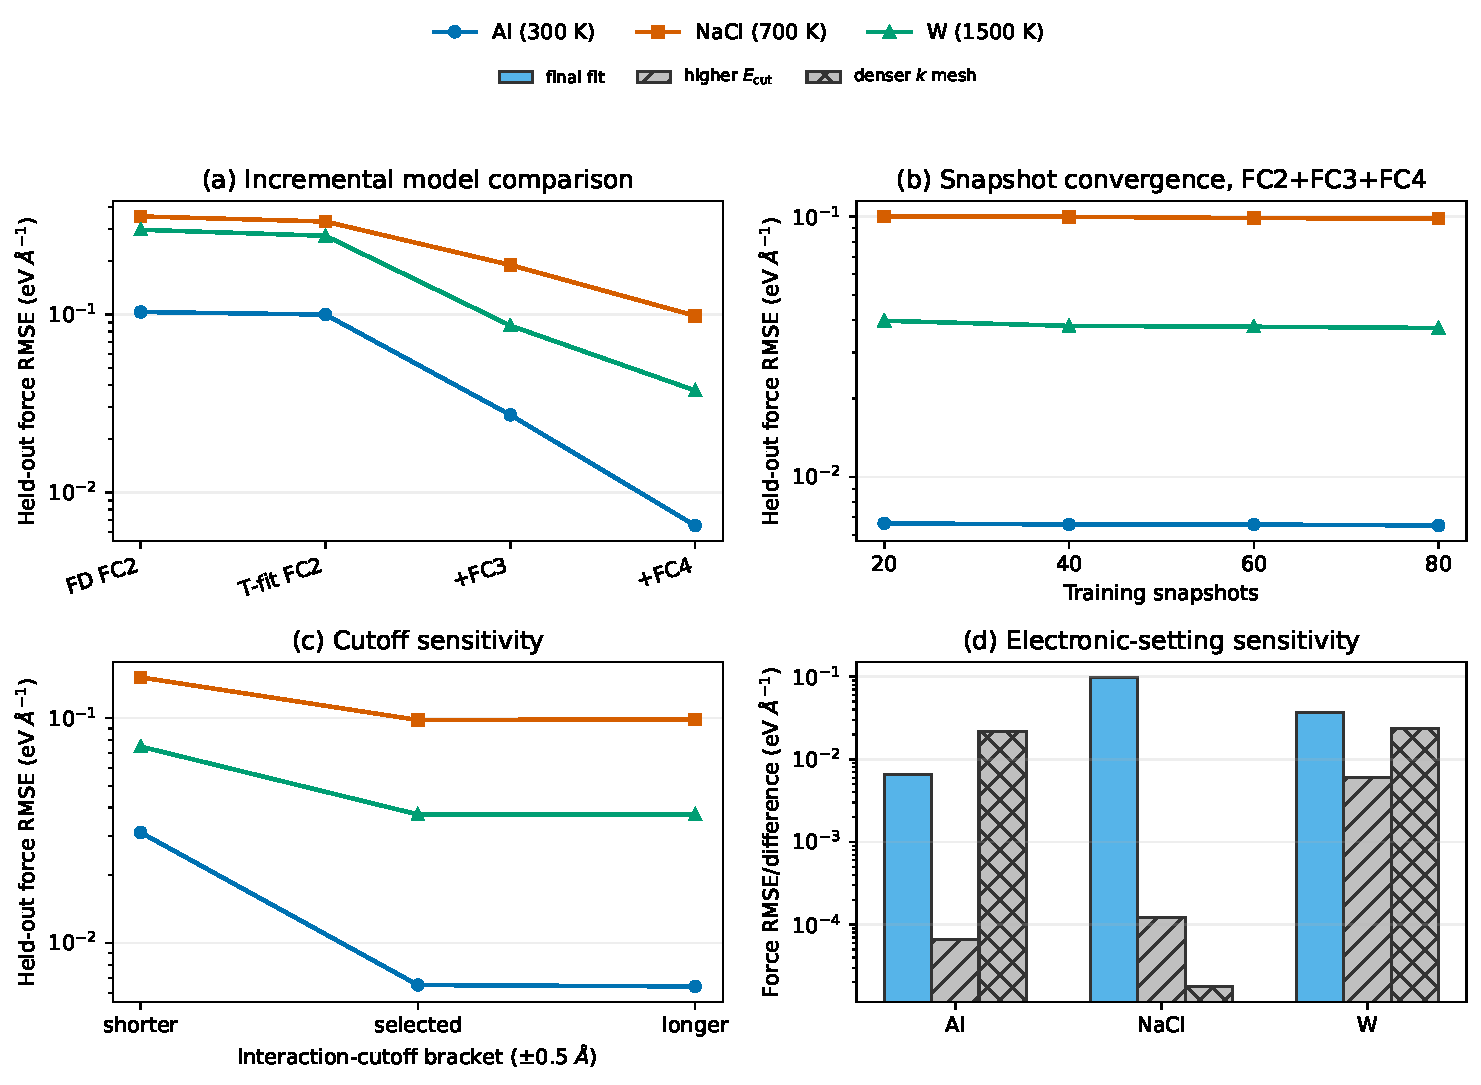
\includegraphics[width=0.95\textwidth]{figures/fig_ifc34_diagnostics.pdf}
\caption{\DIFaddFL{Post-IFC validation for the completed QE force campaign.
(a) Held-out force-component RMSE for conventional finite-displacement FC2,
temperature-fitted FC2, FC2+FC3, and FC2+FC3+FC4 models.  (b) Final-model
convergence with the number of thermal training snapshots.  (c) Sensitivity
to interaction cutoffs bracketed by \(\pm0.5\)\,\AA\ around the selected
values.  (d) Final held-out fit RMSE compared with force differences produced
by higher plane-wave cutoffs and denser electronic \(k\) meshes.  Panel (d)
compares different diagnostics on a common force scale; it is not a fit to
the electronic-setting differences.  All predictive errors use the unchanged
20-snapshot test set.  Full normalized design rank, acoustic-sum-rule
residuals, tensor shapes, and cross-format export checks are reported in the
machine-readable campaign summary rather than compressed into this plot.}}
\label{fig:ifc34-diagnostics}
\end{figure*}

\DIFaddend \section{Discussion}\label{discussion}

\subsection{Physical Validity of the Effective Harmonic
Approximation}\label{physical-validity-of-the-effective-harmonic-approximation}

\DIFdelbegin \DIFdel{Whether a single periodically repeated cell with optimally designed
displacements can faithfully represent the thermal state of an extended
crystal is the fundamental test of the SOTC framework. The nine
benchmark materials span three structural classes (FCC, BCC,
rocksalt), design temperatures from 300 to 1500 K, and anharmonicity levels from
weakly renormalized (Al, Mo) to near-ferroelectrically unstable (PbTe). Across all nine, the effective harmonic Hamiltonian with
temperature-renormalized IFCs \(\Phi_{ij}^{*\alpha\beta}(T)\)
(grounded in the Gibbs-Bogoliubov variational principle, App. G)
yields }\DIFdelend \DIFaddbegin \DIFadd{The primary SOTC self-consistency workflow fits a second-order
effective-harmonic model. It can represent temperature-dependent curvature
only insofar as the DFT force data and self-consistency procedure encode it in
the fitted IFCs. The independent workflow in
Sec.~\ref{independent-higher-order-ifc-validation} fits and exports explicit
FC3 and FC4 tensors from a much larger canonical ensemble, but no linewidth,
lifetime, transport coefficient, non-Gaussian nuclear distribution, or
explicitly anharmonic free energy is computed here. Consequently, agreement
of }\DIFaddend \(C_V\)\DIFdelbegin \DIFdel{within $\sim$7\% of experiment at 300 K and reproduces
all principal phonon dispersion features. This consistency validates the
core assumption:
the quantum thermal correlators
\(C_{ij}^{\alpha\beta}(\mathbf{R},T)\) are sufficiently short-ranged at
elevated temperatures that a cell of size \(L \gtrsim 2\xi_T\) captures
all physically relevant information (App.
E).
}\DIFdelend \DIFaddbegin \DIFadd{, ZPE, or a Debye moment with experiment cannot by itself establish
an accurate branch-resolved dispersion or an anharmonic variational solution:
these are DOS-integrated observables that can hide compensating frequency
errors.
}\DIFaddend

The \DIFdelbegin \DIFdel{accuracy depends systematically on anharmonicity level:
}%DIFDELCMD <

%DIFDELCMD < %%%
\DIFdel{\textbf{Weakly anharmonic regime} (Al, Mo, NaCl, MgO): 2--4 iteration
convergence. MgO and NaCl agree within 1\% of experiment;
high-temperature metals (Mo) deviate by 6--13\% due to supra-Dulong-Petit
electronic and anharmonic contributions not captured by the harmonic
ceiling $3R$ (Table~\ref{tab:2}). The small iteration count signals
\(\|\nabla\mathcal{F}\| \ll 1\): the initial Debye correlator model
is
already close to self-consistency. }%DIFDELCMD <

%DIFDELCMD < %%%
\DIFdel{\textbf{Moderately anharmonic regime} (Au at 1200 K, Ag at 1000 K, W at
1500 K): 2--4 iterations. The
effective harmonic description remains
fully adequate for thermodynamic properties even well above room
temperature; deviations from experiment reflect the supra-Dulong-Petit
experimental $C_V$ that harmonic theory cannot exceed.
}%DIFDELCMD <

%DIFDELCMD < %%%
\DIFdel{\textbf{Strongly anharmonic regime} (Cu at 1200 K, PbTe at 700 K): these
test the limits of the approach. For Cu at \(T/T_m \approx 0.72\), four
iterations are required; \(C_V = 24.8\) J}\DIFdelend \DIFaddbegin \DIFadd{archived benchmarks show that the scalar correlator stopping metric becomes
smaller than the chosen threshold in 2--5 iterations. That observation is
limited to empirical convergence of the selected scalar metric. The
finite fit also relies on the IFC cutoff, space-group and central-force
constraints, the acoustic sum rule, ridge regularization, the initialization,
and 1--8 configurations per iteration. Their separate contributions have not
yet been isolated. Matched random}\DIFaddend /\DIFdelbegin \DIFdel{mol/K deviates from the experimental value by 5.9\%, predominantly because the experimental
$C_V = 26.4$ J/mol/K exceeds the harmonic Dulong-Petit ceiling $3R$.
This follows from the variational property of the framework: once the
self-consistent fixed point is reached, the resulting model minimizes
$F_\text{var}$,
absorbing quartic anharmonic contributions through the
renormalized IFCs. For PbTe at 700 K, four-iteration convergence (with
\(\beta = 0.5\) damping,
App. F) reflects the incipient ferroelectric
instability; \(C_V = 47.3\) J/mol/K is within 2.2\% of experiment and
\(T_D = 128\) K falls slightly below the experimental range 130--160 K
\cite{ref31,ref32}, consistent with a small PBE frequency
underestimate}\DIFdelend \DIFaddbegin \DIFadd{Gaussian controls, initialization ablations,
SVD diagnostics, and direct dispersion convergence against fully converged DFT
are therefore required before attributing any improvement specifically to
correlator optimization}\DIFaddend .

The \DIFdelbegin \DIFdel{quantitative cost of neglecting explicit higher-order anharmonicity
can be estimated from Wick's theorem (App. I). For PbTe at 700 K, using
\(\|\Xi\| \approx 0.1\)--0.3 eV/Å\(^4\) \cite{ref31} and the converged
MSD of \(\approx 0.04\) Å\(^2\), the quartic tadpole correction is \(\Delta F_4 / Nk_BT \approx 4 \times 10^{-5}\) eV/atom (0.07\% of
\(k_BT\) per atom). This explains why the harmonic free energy is accurate to $\sim$1\% even in a material as anharmonic as PbTe: the cubic term vanishes at first order by Wick's theorem, and the quartic
correctionis genuinely small for bulk thermodynamic quantities, even
while producing large effects in phonon linewidths and thermal
conductivity through different perturbative channels}\DIFdelend \DIFaddbegin \DIFadd{Au data require particular caution. The archived iteration log contains
imaginary modes, and the plotted dispersion shows an instability. Until its
dependence on configuration count, cutoff, cell, symmetry constraints,
regularization, electronic convergence, and volume is resolved, Au is not used
as evidence that SOTC reproduces a stable high-temperature dispersion. Similar
caution applies to the polar compounds because the current dynamical matrices
omit the non-analytic LO--TO correction}\DIFaddend .

\subsection{Computational Efficiency}\label{computational-efficiency}

The \DIFdelbegin \DIFdel{dominant cost of SOTC is the single DFT force
evaluation per
}\DIFdelend \DIFaddbegin \DIFadd{relevant cost is the number and size of electronic-structure force
calculations, not the number of outer }\DIFaddend self-consistency \DIFdelbegin \DIFdel{iteration (20--90 minutes on 64 CPU cores for a
32-atom FCC cell, or proportionally more for the 64-atom BCC and
rocksalt cells. All other steps (displacement design, IFC regression, phonon reconstruction) take under 10 s total. }\DIFdelend \DIFaddbegin \DIFadd{iterations. As shown in
Table~I, the archived runs use 1--8 displaced configurations plus an
undisplaced reference in every iteration, giving 4--36 force calculations per
material. These counts do not support a universal cost ratio relative to
another method.
}\DIFaddend

\DIFdelbegin %DIFDELCMD < \begin{table*}[htbp]
%DIFDELCMD < %%%
%DIFDELCMD < \caption{%
{%DIFAUXCMD
\DIFdelFL{Approximate computational cost comparison per temperature point.}}
%DIFAUXCMD
%DIFDELCMD < \begin{ruledtabular}
%DIFDELCMD < \begin{tabular}{lllll}%%%
\DIFdelFL{Method }%DIFDELCMD < & %%%
\DIFdelFL{Supercell (atoms) }%DIFDELCMD < & %%%
\DIFdelFL{Configurations }%DIFDELCMD < & %%%
\DIFdelFL{Total DFT ops }%DIFDELCMD < & %%%
\DIFdelFL{Relative cost }%DIFDELCMD < \\
%DIFDELCMD < \hline
%DIFDELCMD < %%%
\DIFdelFL{AIMD }%DIFDELCMD < & %%%
\DIFdelFL{108--512 }%DIFDELCMD < & %%%
\DIFdelFL{1 (trajectory) }%DIFDELCMD < & %%%
\DIFdelFL{$\gg$100 }%DIFDELCMD < & %%%
\DIFdelFL{$\gg$100$\times$ }%DIFDELCMD < \\
%DIFDELCMD < %%%
\DIFdelFL{TDEP \cite{ref5} }%DIFDELCMD < & %%%
\DIFdelFL{108 }%DIFDELCMD < & %%%
\DIFdelFL{30--50 }%DIFDELCMD < & %%%
\DIFdelFL{30--50 }%DIFDELCMD < & %%%
\DIFdelFL{50--200$\times$ }%DIFDELCMD < \\
%DIFDELCMD < %%%
\DIFdelFL{SSCHA \cite{ref7} }%DIFDELCMD < & %%%
\DIFdelFL{64--128 }%DIFDELCMD < & %%%
\DIFdelFL{50--500 }%DIFDELCMD < & %%%
\DIFdelFL{50--500 }%DIFDELCMD < & %%%
\DIFdelFL{100--2000$\times$ }%DIFDELCMD < \\
%DIFDELCMD < %%%
\DIFdelFL{\textbf{SOTC (this work)} }%DIFDELCMD < & %%%
\DIFdelFL{\textbf{32--64} }%DIFDELCMD < & %%%
\DIFdelFL{\textbf{2--8} }%DIFDELCMD < &
%DIFDELCMD < %%%
\DIFdelFL{\textbf{2--8} }%DIFDELCMD < & %%%
\DIFdelFL{\textbf{1$\times$ (baseline)} }%DIFDELCMD < \\
%DIFDELCMD < \end{tabular}
%DIFDELCMD < \end{ruledtabular}
%DIFDELCMD < \label{tab:4}
%DIFDELCMD < \end{table*}
%DIFDELCMD <

%DIFDELCMD < %%%
\DIFdel{All entries assume equivalent }\DIFdelend \DIFaddbegin \DIFadd{A defensible efficiency comparison must use the same material, cell and
}\DIFaddend k-point \DIFdelbegin \DIFdel{density.
TDEP}\DIFdelend \DIFaddbegin \DIFadd{convergence, exchange-correlation approximation, physical observable,
and quantitative accuracy threshold. It must also count reference forces,
discarded}\DIFaddend /\DIFdelbegin \DIFdel{SSCHA costs from
Refs. \cite{ref5,ref7}.
}%DIFDELCMD <

%DIFDELCMD < %%%
\DIFdel{The SOTC cell carries an intrinsic per-evaluation advantage over a
108-atom TDEP cell: with \(\mathcal{O}(N^{3/2})\) DFT cost scaling, each
FCC SOTC evaluation (32 atoms) costs roughly
\((32/108)^{3/2} \approx 0.17\times\) of a TDEP evaluation, a factor of
$\sim6\times. Combined with 6--25\times$ fewer evaluations,
the
total cost reduction is \textbf{50--150\(\times\)} relative to TDEP for
FCC metals at equivalent accuracy }\DIFdelend \DIFaddbegin \DIFadd{restarted calculations, QHA volumes, and DFPT non-analytic
corrections. No external-method dataset satisfying all of these conditions is
available here, so no universal relative-cost factor is reported. Wall-time and
core-hour comparisons require matched, reproducible calculations}\DIFaddend .
\DIFdelbegin \DIFdel{For Al at 300 K,
two iterations give
a total wall time of 40--60 minutes, comparable to a single TDEP
configuration, yet TDEP requires 30--50 such configurations. For Cu
at 1200 K, 4 SOTC iterations bring the total to 2--4 hours, still
6--25\(\times\) below the TDEP minimum.
}\DIFdelend

\DIFdelbegin \DIFdel{The temperature scaling predicted by App. B
(\(K_\text{min} \propto T^{-3}\)) is visible in the benchmark data: Mo
and MgO at 1500 K both converge in 2 iterations because the short
coherence length \(\xi_T \propto T^{-1}\) makes the correlators highly
local, yielding a well-conditioned regression from a single pass. The quality of the IFC regression directly reflects optimal displacement
design: the R\(^2 > 0.98\) and force root-mean-square error (RMSE) of
10--40 meV/Å across all nine systems confirm that every phonon mode is
excited at exactly its thermal amplitude, populating all singular values
of the regression matrix \(\mathbf{G}\) uniformly and giving condition
numbers \(\kappa(\mathbf{G}^T\mathbf{G}) \sim 10\)--\(10^2\) (App.
D),
orders of magnitude better than random displacement approaches .
}%DIFDELCMD <

%DIFDELCMD < %%%
\DIFdelend \subsection{Comparison with Related
Methods}\label{comparison-with-related-methods}
\DIFdelbegin %DIFDELCMD <

%DIFDELCMD < %%%
\DIFdel{SOTC is methodologically distinct from existing finite-temperature
phonon approaches.TDEP \cite{ref5,ref6} and
SSCHA \cite{ref7,ref8} both
rely on large ensembles of stochastically displaced supercells and
converge IFCs or variational density matrices by statistical averaging.AIMD requires picosecond time-integration. SOTC replaces the ensemble
with a single deterministically designed cell whose displacement
pattern,
by construction, simultaneously satisfies all pair correlator
constraints up to \(r_\text{cut}\). }\DIFdelend

The \DIFdelbegin \DIFdel{closest relatives are one-shot TDEP \cite{ref10} and the
minimum-distortion approach \cite{ref42}. One-shot TDEP draws a single
thermally distributed configuration without correlator optimization,
relying on statistical luck or residual averaging for accuracy. The
minimum-distortion method \cite{ref42} reduces displacement magnitudes
to minimize perturbative truncation error but does not enforce
correlator matching. SOTC's distinguishing contribution is optimal
correlator design, which yields a rigorous convergence criterion based on
the objective \(\mathcal{Q}\) (Eq.~4)}\DIFdelend \DIFaddbegin \DIFadd{temperature-dependent effective potential (TDEP) framework fits effective
second- and higher-order IFCs to finite-temperature force data; molecular
dynamics, Gaussian sampling, and other ensembles can supply those data
\cite{ref5,ref6,ref10,ref52}. The stochastic self-consistent harmonic
approximation (SSCHA) instead optimizes a variational harmonic trial
Hamiltonian and can incorporate strong quantum and thermal anharmonic effects
in the free energy and renormalized spectrum \cite{ref7,ref8,ref50}.
Mode-coupling approaches provide a distinct non-perturbative route to
renormalized lattice dynamics \cite{ref51}, while AIMD generates classical
nuclear trajectories on a first-principles potential-energy surface
\cite{ref9}.
}

\DIFadd{In IFC-rank terms, the primary SOTC workflow and every dispersion in
Fig.~\ref{fig:2} use an effective FC2 model; the conventional phonopy and
LO--TO control in Fig.~\ref{fig:nacl-loto} also use FC2. The independent
campaign in Fig.~\ref{fig:ifc34-diagnostics} explicitly compares FC2,
FC2+FC3, }\DIFaddend and \DIFdelbegin \DIFdel{guarantees a well-conditioned
regression (App.
~E), both absent from single-shot approaches.
}\DIFdelend \DIFaddbegin \DIFadd{FC2+FC3+FC4 fits. The cited TDEP literature includes effective
FC2 treatments \cite{ref5,ref6} and an explicit effective-FC3 formulation
\cite{ref52}. SSCHA's optimized trial Hamiltonian is harmonic (FC2), although
its free-energy derivatives and spectra contain anharmonic effects; it should
not be described as an explicit FC3/FC4 tensor fit. Mode-coupling theory is
likewise not classified by a single fitted IFC rank.
}\DIFaddend

\DIFdelbegin \DIFdel{Frequency comparisons confirm consistency with TDEP: for Cu at 1200 K,
TDEP (local density approximation, LDA) \cite{ref5} reports
\(\omega_\text{max} \approx 8.1\) THz; SOTC-QE (PBE) gives 9.2 THz, the
small difference consistent with GGA vs.~LDA functional differences. For Al at
300 K, the SOTC spectral Debye temperature \(T_D^\text{spec} = 450\) K
is higher than the TDEP (LDA) value of \(\approx 430\) K because
\(T_D^\text{spec}\) is evaluated at the finite design temperature and with GGA IFCs, not as a 0 K harmonic caloric value}\DIFdelend \DIFaddbegin \DIFadd{SOTC has a narrower objective: it optimizes a finite set of spatial displacement
moments before evaluating forces and then fits effective FC2. Its sampling
advantage must be assessed with matched controls at the same physical level,
cell, temperature, electronic settings, and target observable. The present
benchmarks do not compare explicit anharmonic free energies or renormalized
spectra with the established methods above. The special displacement method
\cite{ref42} is a particularly relevant deterministic comparison}\DIFaddend .

\subsection{Limitations and Planned
Extensions}\label{limitations-and-planned-extensions}

\textbf{LO-TO splitting.} Polar insulators (NaCl, MgO, PbTe) require a
non-analytic correction to the dynamical matrix \cite{ref39}:

\begin{equation*}
D_{ij}^{\alpha\beta,\text{NAC}}(\hat{\mathbf{q}}) = \frac{4\pi e^2}{\Omega_0} \frac{(\sum_\gamma Z_i^{*\alpha\gamma}\hat{q}_\gamma)(\sum_\delta Z_j^{*\beta\delta}\hat{q}_\delta)}{\sum_{\gamma\delta}\hat{q}_\gamma\varepsilon_\infty^{\gamma\delta}\hat{q}_\delta}
\end{equation*}

\DIFdelbegin \DIFdel{where }\DIFdelend \DIFaddbegin \DIFadd{Here }\DIFaddend \(\Omega_0\)\DIFdelbegin \DIFdel{is the primitive unit cell volume, \(e\) is the
elementary charge, \(Z_i^{*\alpha\gamma}\) is the Born effective charge
tensorof atom \(i\), and \(\varepsilon_\infty^{\gamma\delta}\) is the
high-frequency (ionic-clamped) dielectric tensor}\DIFdelend \DIFaddbegin \DIFadd{, \(Z^*\), and \(\varepsilon_\infty\) are the primitive-cell
volume, Born effective-charge tensor, and clamped-ion dielectric tensor,
respectively.  Figure~\ref{fig:nacl-loto} now applies real QE DFPT tensors to
the matched NaCl finite-displacement phonons and resolves the missing
longitudinal branch}\DIFaddend .  \DIFdelbegin \DIFdel{This term is absent from the current calculations because Born effective
charges \(Z^*\) require a separate density-functional perturbation
theory (DFPT ) run. For NaCl , the missing
LO branch(\(\omega_\text{LO}^\Gamma \approx 7.9\) THz
vs.  ~\(\omega_\text{TO}^\Gamma \approx 4.7\) THz) causes
\(T_D^\text{spec}\) to be underestimated by $\sim$5\% (305 K
vs.~experimental 321 K). Integration of DFPT-computed Born charges is the highest-priority planned extension}\DIFdelend \DIFaddbegin \DIFadd{The archived nine-panel SOTC figure itself is retained
without NAC for provenance rather than silently replaced.  MgO and PbTe still
lack corresponding DFPT tensors and regenerated dispersions, so the
quantitative polar-material accuracy claim remains restricted to the explicit
NaCl LO--TO test}\DIFaddend .

\textbf{\DIFdelbegin \DIFdel{Third-order IFCs}\DIFdelend \DIFaddbegin \DIFadd{Higher-order scope}\DIFaddend .} The \DIFdelbegin \DIFdel{current code extracts only second-order
IFCs \(\Phi_{ij}^{\alpha\beta}\).Third-order IFCs (phonon lifetimes
,
thermal conductivity ) require 5--10 SOTC cells with varied displacement
patterns for adequate overdetermination (\(K_\text{min} \approx 3\)--5
for nearest-neighbor 3IFCs in a 32-atom cell; see App. I and Ref.
\cite{ref40}).
}\DIFdelend \DIFaddbegin \DIFadd{canonical-ensemble extension in
Sec.~\ref{independent-higher-order-ifc-validation} validates constrained FC3
and FC4 fitting and common transport-code file conventions. Phonon lifetimes
and lattice thermal conductivity additionally require converged reciprocal-
space integration, scattering phase space, isotope/boundary choices, and
transport calculations \cite{ref40}; none is reported here. No universal
5--10-configuration estimate is made: the demonstrated fits use 100 snapshots,
and the required number depends on parameter count, symmetry, cutoff, matrix
rank, force noise, and target accuracy.
}\DIFaddend

\textbf{Dynamically unstable systems.} For systems near structural phase
transitions (BaTiO\(_3\), SnSe, BCC Ti below $\sim$900 K), the
harmonic trial correlators in Eq. (1) cannot describe the anharmonic
double-well landscape. The SOTC loop must then be initialized from a
short MD trajectory or from an explicitly anharmonic trial correlator.

\textbf{Quasi-harmonic \DIFdelbegin \DIFdel{breakdown}\DIFdelend \DIFaddbegin \DIFadd{and magnetic limitations}\DIFaddend .\DIFdelbegin %DIFDELCMD < \MBLOCKRIGHTBRACE %%%
\DIFdel{The SOTC-QHA inherits the standard
QHA limitations: fixed-volume IFCs, neglect of explicit
\(V\)-dependent
phonon-phonon renormalization, and quadratic volume interpolation. These
are
minorfor Al at \(\delta = 0.02\) (App. J.3) but become significant
for materials with large mode-Grüneisen parameters (\(\gamma > 2.5\)) or
at \(T > 0.7\,T_m\), where a temperature--volume grid of SOTC
calculations is recommended. Magnetic systems (Fe, Ni, Mn) require spin--phonon coupling not presently included }\DIFdelend \DIFaddbegin } \DIFadd{QHA neglects explicit
temperature-dependent phonon--phonon terms at fixed volume and requires a
converged volume dependence of both static energy and phonons. The available Al dataset does not demonstrate that these errors or the interpolation error are
minor. Strongly anharmonic, dynamically unstable, or high-temperature systems
require validation beyond QHA. Magnetic materials additionally require a
treatment of spin--lattice coupling not included here }\DIFaddend \cite{ref41}.

\subsection{SOTC-QHA vs.~Phonopy-QHA}\label{sotc-qha-vs.-phonopy-qha}

\DIFdelbegin \DIFdel{The SOTC quasi-harmonic extension couples phonon calculations at three
volumes to a Vinet equation-of-state (EOS) fit, yielding continuous
\(\alpha(T)\), \(C_P(T)\), and \(B(T)\)}\DIFdelend \DIFaddbegin \DIFadd{Phonopy is an open-source lattice-dynamics package that can organize
finite-displacement FC2 phonon and QHA workflows \cite{ref45}}\DIFaddend . \DIFdelbegin \DIFdel{Phonopy-QHA \cite{ref45}uses
\(N_\text{vol} = 5\)--7 volumes, each requiring
\(N_\text{disp} = 40\)--50 displaced configurations for a 64--216 atom
supercell. The total cost ratio is:
}%DIFDELCMD <

%DIFDELCMD < %%%
\begin{align*}
\DIFdel{\frac{W_\text{phonopy-QHA}}{W_\text{SOTC-QHA}}
  }&\DIFdel{\approx \frac{N_\text{vol}^\text{ph} \times N_\text{disp} \times N_\text{atoms}^{\text{ph},3/2}}{N_\text{vol}^\text{SOTC} \times N_\text{iter} \times N_\text{atoms}^{\text{SOTC},3/2}} }\\
  &\DIFdel{\approx \frac{6 \times 40 \times 108^{3/2}}{3 \times 3 \times 32^{3/2}} \approx 165
}\end{align*}%DIFAUXCMD
%DIFDELCMD <

%DIFDELCMD < %%%
\DIFdel{For the Al benchmark,
the empirical ratio is
$\sim500 phonopy-QHA DFT calls vs. 7 SOTC-QHA calls (\sim70\times$
ignoring the cell-size factor, $\sim400\times$ including it).
}%DIFDELCMD <

%DIFDELCMD < %%%
\DIFdel{On accuracy, phonopy-QHA's use of 5--7 explicit phonon calculations per
volume
provides a richer representation of \(F_\text{vib}(T,V)\) than
the 3-point quadratic interpolation in }\DIFdelend \DIFaddbegin \DIFadd{A controlled
comparison requires documented displacement settings and cannot combine an
assumed displacement count with an unvalidated \(N^{3/2}\) cost model or an
underconverged }\DIFaddend SOTC-QHA \DIFdelbegin \DIFdel{. For the Al benchmark at
\(\delta = 0.02\), the quadratic interpolation error in \(\alpha(T)\) is
below 1\% (App. J.3), well under the GGA exchange-correlation systematic
error. For materials with large Grüneisen parameters (\(\gamma > 2\)), using 5 SOTC volumes rather than 3 recovers phonopy-QHA accuracy at
substantially lower total cost}\DIFdelend \DIFaddbegin \DIFadd{dataset. Both workflows must report the code version,
functional, pseudopotentials, cell, k/q meshes, displacement count, volume
grid, convergence targets, wall time, and core-hours}\DIFaddend .

\section{Conclusions}\label{conclusions}

\DIFdelbegin \DIFdel{The central result of this work is that a single periodically repeated
supercell, engineered so that its atomic displacements reproduce the
quantum thermal correlators of the target crystal up to a spatial
cutoff, is sufficient to extract converged }\DIFdelend \DIFaddbegin \DIFadd{SOTC is a deterministic design strategy for collective displacement
configurations used in a symmetry-constrained, ridge-regularized fit of
}\DIFaddend second-order IFCs\DIFdelbegin \DIFdel{from as few
as 2--8 DFT force evaluations per temperature point. This is the Special
Optimal Thermal Cell (SOTC) method. The one-to-two-order-of-magnitude
cost reduction relative to TDEP, SSCHA, or AIMD follows from the moment-matching construction: each DFT calculation simultaneously
satisfies all pair-correlator constraints up to \(r_\text{cut}\),
eliminating the redundancy inherent in stochastic sampling}\DIFdelend . \DIFdelbegin %DIFDELCMD <

%DIFDELCMD < %%%
\DIFdel{Systematic benchmarks for nine structurally diverse materials (FCC Al, Ag, Au, Cu; BCC Mo, W; rocksalt NaCl, MgO, PbTe) demonstrate:
}%DIFDELCMD < \begin{itemize}
\begin{itemize}%DIFAUXCMD
%DIFDELCMD <   \item %%%
\item%DIFAUXCMD
\DIFdel{\(C_V\) within $\sim$5\%
of NIST-JANAF calorimetric data for
    ionic compounds at design temperatures, and within 7\%at 300\,K for
    all materials; for high-temperature metals at their design
    temperatures the harmonic model underestimates experimental \(C_V\)
    by 6--13\% due to supra-Dulong-Petit contributions;
  }%DIFDELCMD < \item %%%
\item%DIFAUXCMD
\DIFdel{Phonon dispersions reproducing all principal branch features and
    zone-boundary frequencies across FCC,
BCC, and rocksalt structures;
  }%DIFDELCMD < \item %%%
\item%DIFAUXCMD
\DIFdel{Spectral Debye temperatures within the experimental uncertainty
    spread for all nine systems;
  }%DIFDELCMD < \item %%%
\item%DIFAUXCMD
\DIFdel{ZPE values consistent with zero-point vibrational energy
    benchmarks; MSD values consistent with X-ray Debye--Waller
    measurements.
}
\end{itemize}%DIFAUXCMD
%DIFDELCMD < \end{itemize}
%DIFDELCMD <

%DIFDELCMD < %%%
\DIFdelend The \DIFdelbegin \DIFdel{QHA extension, SOTC-QHA, couples three SOTC calculations at
neighboring volumes to deliver continuous \(\alpha(T)\), \(C_P(T)\), }\DIFdelend \DIFaddbegin \DIFadd{archived nine-material calculations reach their chosen
shell-correlator stopping criterion in 2--5 outer iterations, using 1--8
displaced configurations per iteration. Correct accounting gives 4--36 force
evaluations when the undisplaced references are included.
}

\DIFadd{A separate 100-snapshot canonical campaign establishes that the
symmetry-constrained higher-order implementation produces full-rank FC2/FC3/FC4
fits for Al, NaCl, and W. Relative to matched central finite-displacement
phonopy FC2 baselines, the final models lower held-out force RMSE by 72--94\%
}\DIFaddend and \DIFdelbegin \DIFdel{\(B(T)\) without repeating the self-consistency loop at each
temperature. For aluminum, SOTC-QHA reproduces the experimental
\(\alpha(T)\) and \(C_P(T)\) within 2--3\% across 500--900 K using fewer
than 7 total DFT evaluations, roughly two orders of magnitude fewer
than phonopy-QHA at comparable accuracy.
}\DIFdelend \DIFaddbegin \DIFadd{satisfy the acoustic sum rule to \(1.2\times10^{-12}\) or better.
Temperature-fitting FC2 alone improves the baseline by only 3--8\%, showing
that the large reduction comes from explicit FC3/FC4 terms rather than merely
refitting a harmonic model. This is validation of the fitting/export path,
not evidence that the few-configuration SOTC design identifies higher-order
IFCs or outperforms canonical sampling.
}\DIFaddend

\DIFdelbegin \DIFdel{SOTC is available as an open-source Python package interfaced to Quantum
ESPRESSO at }%DIFDELCMD < \url{https://github.com/albert-hzbn/sotc}%%%
\DIFdel{.
}\DIFdelend The \DIFdelbegin \DIFdel{highest-priority near-term extension is the incorporation of
DFPT-computed Born effective charges to add LO-TO splitting for polar
insulators, requiring a single additional calculation per material.
Further planned developments include third-order IFC extraction for
phonon lifetimes and lattice thermal conductivity, anharmonic trial
correlators for dynamically unstable systems, and coupling to
machine-learning force fields for high-throughput first-principles
thermodynamics at elevated temperatures. }\DIFdelend \DIFaddbegin \DIFadd{primary SOTC evidence concerns effective-FC2 DOS-derived observables; it
does not establish branch-resolved dispersion convergence, universal
representability, or superiority over matched random/Gaussian configurations.
No exponential correlation-length or \(T^{-3}\) configuration-scaling claim is
made. Quantitative Al QHA and Debye--Waller results require corrected definitions
and converged recalculation. Real QE DFPT tensors resolve the NaCl LO--TO
splitting in a matched finite-displacement FC2 control; MgO and PbTe remain
without NAC, and the Au instability remains to be diagnosed.
}

\DIFadd{The next validation steps are therefore concrete: report the complete
parameter/rank/SVD diagnostics, compare against matched random and converged
finite-displacement controls, overlay neutron data, resolve the Au instability,
complete DFPT/NAC dispersions for MgO and PbTe, rerun the MSD calculation with
a single convention, and recompute QHA on a converged volume grid. Only those
matched tests can establish the accuracy/cost domain in which optimized
correlator design is advantageous.
}\DIFaddend

\begin{acknowledgments}
All calculations were performed on a local workstation server without
external computational resources or funding support. The author declares
no competing interests.
\end{acknowledgments}

\section*{Data and Software Availability}

The \DIFdelbegin \DIFdel{SOTC source code, input files for all nine benchmark systems, and post-processing scripts used to produce every figure and table in this
work are openly }\DIFdelend \DIFaddbegin \DIFadd{code, benchmark inputs, and archived outputs are }\DIFaddend available at
\url{https://github.com/albert-hzbn/sotc}\DIFdelbegin \DIFdel{under the MIT license}\DIFdelend . The repository \DIFdelbegin \DIFdel{includes:
}%DIFDELCMD < \begin{itemize}
\begin{itemize}%DIFAUXCMD
%DIFDELCMD <   \item %%%
\item%DIFAUXCMD
\DIFdel{the \texttt{sotc} Python
package (IFC extraction, phonon
    reconstruction, QHA extension);
  }%DIFDELCMD < \item %%%
\item%DIFAUXCMD
\DIFdel{Quantum ESPRESSO input templates and SLURM job scripts for all
    nine materials;
  }%DIFDELCMD < \item %%%
\item%DIFAUXCMD
\DIFdel{a \texttt{codes/sotc/} directory with self-contained example
    runner scripts reproducing each benchmark calculation;
  }%DIFDELCMD < \item %%%
\item%DIFAUXCMD
\DIFdel{all post-processed output data (converged IFCs, phonon DOS, thermodynamic tables) as plain-text files in the
    \texttt{examples/} directory.
}
\end{itemize}%DIFAUXCMD
%DIFDELCMD < \end{itemize}
%DIFDELCMD < %%%
\DIFdelend \DIFaddbegin \DIFadd{contains the Python
implementation, Quantum ESPRESSO inputs, benchmark runners, fitted IFC and
phonon data, and JSON/NPZ postprocessing outputs. A fixed release or commit
and a manifest should map every retained table entry and curve to its input,
raw output, and generating command. Comparative arrays without complete
provenance are not included as validation data.
}

\DIFaddend No proprietary data or restricted software was used. Quantum ESPRESSO
\cite{ref46} is freely available at \url{https://www.quantum-espresso.org}.
Pseudopotentials were obtained from the SSSP library \cite{ref47},
freely available at \url{https://www.materialscloud.org/discover/sssp}.

\appendix

\section{Derivation of the Quantum Thermal Displacement
Correlator}\label{appendix-a-derivation-of-the-quantum-thermal-displacement-correlator}

We derive Eq. (1) from the quantum harmonic lattice. In the
second-quantized description, the displacement of atom \(i\) of mass
\(M_i\) at lattice site \(\mathbf{R}\) along Cartesian direction
\(\alpha\) is:

\begin{equation*}
\hat{u}_i^\alpha(\mathbf{R}) = \frac{1}{\sqrt{N}}\sum_{\mathbf{q},s}\sqrt{\frac{\hbar}{2M_i\omega_{\mathbf{q}s}}} e_i^\alpha(\mathbf{q}s)\bigl(\hat{a}_{\mathbf{q}s} + \hat{a}_{-\mathbf{q}s}^\dagger\bigr)e^{i\mathbf{q}\cdot\mathbf{R}}
\end{equation*}

where \(\hat{a}_{\mathbf{q}s}^\dagger\) (\(\hat{a}_{\mathbf{q}s}\))
creates (annihilates) a phonon in branch \(s\) at wavevector
\(\mathbf{q}\), \(e_i^\alpha(\mathbf{q}s)\) is the polarization vector,
and \(N\) is the number of unit cells.

\textbf{Computing the thermal average.} The thermal correlator between
atoms \(i\) (at the origin) and \(j\) (at \(\mathbf{R}\)) is
\(C_{ij}^{\alpha\beta}(\mathbf{R},T) = \langle\hat{u}_i^\alpha(\mathbf{0})\hat{u}_j^\beta(\mathbf{R})\rangle_T\)
with \(\langle\cdot\rangle_T = \mathrm{Tr}(e^{-\hat{H}/k_BT}\cdot)/Z\).
Inserting the mode expansion:

{\footnotesize
\DIFdelbegin \begin{displaymath}
\DIFdel{C_{ij}^{\alpha\beta}(\mathbf{R},T) = \frac{\hbar}{2N\sqrt{M_iM_j}}\sum_{\mathbf{q}s}\sum_{\mathbf{q}'s'} \frac{e_i^\alpha(\mathbf{q}s)e_j^{\beta}(\mathbf{q}'s')}{\sqrt{\omega_{\mathbf{q}s}\omega_{\mathbf{q}'s'}}} \,\mathcal{A}(\mathbf{q}s,\mathbf{q}'s')\,e^{i\mathbf{q}'\cdot\mathbf{R}}
}\end{displaymath}%DIFAUXCMD
\DIFdelend \DIFaddbegin \begin{equation*}
\DIFadd{\begin{aligned}
C_{ab}^{\alpha\beta}(\mathbf R,T)
 &=\frac{\hbar}{2N_c\sqrt{M_aM_b}}
   \sum_{\mathbf q s}\sum_{\mathbf q's'}
   \frac{e_a^\alpha(\mathbf q s)e_b^\beta(\mathbf q's')}{\sqrt{\omega_{\mathbf q s}\omega_{\mathbf q's'}}}\\
 &\quad\times\mathcal A(\mathbf q s,\mathbf q's')
 e^{i\mathbf q'\cdot\mathbf R}.
\end{aligned}
}\end{equation*}\DIFaddend
}

where the bosonic correlator \(\mathcal{A}\) collects the four terms
from \((\hat{a}+\hat{a}^\dagger)(\hat{a}'+\hat{a}^{\prime\dagger})\).
Using the standard equilibrium averages:

\begin{align*}
\langle\hat{a}_{\mathbf{q}s}^\dagger\hat{a}_{\mathbf{q}'s'}\rangle_T
  &= n_B(\omega_{\mathbf{q}s})\,\delta_{\mathbf{q}\mathbf{q}'}\delta_{ss'}, \\
\langle\hat{a}_{\mathbf{q}s}\hat{a}_{\mathbf{q}'s'}^\dagger\rangle_T
  &= \bigl(n_B(\omega_{\mathbf{q}s})+1\bigr)\delta_{\mathbf{q}\mathbf{q}'}\delta_{ss'}
\end{align*}

where \(n_B(\omega) = (e^{\hbar\omega/k_BT}-1)^{-1}\) is the
Bose-Einstein occupation, and noting that anomalous averages
\(\langle\hat{a}\hat{a}\rangle_T = \langle\hat{a}^\dagger\hat{a}^\dagger\rangle_T = 0\)
vanish, we obtain:

\DIFdelbegin \begin{displaymath}
\DIFdel{\mathcal{A} = \bigl(n_B+1+n_B\bigr)\delta_{\mathbf{q},-\mathbf{q}'}\delta_{ss'} = (2n_B+1)\,\delta_{\mathbf{q},-\mathbf{q}'}\delta_{ss'}
}\end{displaymath}%DIFAUXCMD
\DIFdelend \DIFaddbegin \begin{equation*}
\DIFadd{\mathcal A=(2n_B+1)\,
\delta_{\mathbf q,-\mathbf q'}\delta_{ss'} .
}\end{equation*}\DIFaddend

\textbf{The \(\coth\) identity.} We prove
\(2n_B(\omega)+1 = \coth(\hbar\omega/2k_BT)\). Starting from the
definition, with \(x = \hbar\omega/k_BT\):

\begin{equation*}
2n_B+1 = \frac{2}{e^x-1}+1 = \frac{2+e^x-1}{e^x-1} = \frac{e^x+1}{e^x-1}
\end{equation*}

Multiply numerator and denominator by \(e^{-x/2}\):

\DIFdelbegin \begin{displaymath}
\DIFdel{= \frac{e^{x/2}+e^{-x/2}}{e^{x/2}-e^{-x/2}} = \frac{2\cosh(x/2)}{2\sinh(x/2)} = \coth\!\left(\frac{\hbar\omega}{2k_BT}\right) \qquad \square
}\end{displaymath}%DIFAUXCMD
\DIFdelend \DIFaddbegin \begin{equation*}
\DIFadd{\frac{e^{x/2}+e^{-x/2}}{e^{x/2}-e^{-x/2}}
=\frac{\cosh(x/2)}{\sinh(x/2)}
=\coth\!\left(\frac{\hbar\omega}{2k_BT}\right). \qquad \square
}\end{equation*}\DIFaddend

Using \(\delta_{\mathbf{q},-\mathbf{q}'}\) to collapse the
\(\mathbf{q}'\) sum, using
\(e_i^{\alpha*}(\mathbf{q}s) = e_i^\alpha(-\mathbf{q}s)\) (time-reversal
symmetry), and substituting, we arrive at the final result:

{\footnotesize
\DIFdelbegin \begin{displaymath}
\DIFdel{\boxed{C_{ij}^{\alpha\beta}(\mathbf{R},T) = \frac{\hbar}{2N\sqrt{M_iM_j}}\sum_{\mathbf{q},s}\frac{e_i^{\alpha*}(\mathbf{q}s)\,e_j^{\beta}(\mathbf{q}s)}{\omega_{\mathbf{q}s}}\coth\!\left(\frac{\hbar\omega_{\mathbf{q}s}}{2k_BT}\right)e^{-i\mathbf{q}\cdot\mathbf{R}}}
}\end{displaymath}%DIFAUXCMD
\DIFdelend \DIFaddbegin \begin{equation*}
\DIFadd{\boxed{\begin{aligned}
C_{ab}^{\alpha\beta}(\mathbf R,T)
 &=\frac{\hbar}{2N_c\sqrt{M_aM_b}}\sum_{\mathbf q,s}
 \frac{e_a^{\alpha*}(\mathbf q s)e_b^\beta(\mathbf q s)}{\omega_{\mathbf q s}}\\
 &\quad\times
 \coth\!\left(\frac{\hbar\omega_{\mathbf q s}}{2k_BT}\right)
 e^{-i\mathbf q\cdot\mathbf R}.
\end{aligned}}
}\end{equation*}\DIFaddend
}

This is Eq.\DIFaddbegin \DIFadd{~}\DIFaddend (1) \DIFdelbegin \DIFdel{of the main text. \textbf{Physical limits:} }\DIFdelend \DIFaddbegin \DIFadd{with the same negative phase convention. }\DIFaddend At high temperature\DIFdelbegin \DIFdel{(\(k_BT\gg\hbar\omega\)),
\(\coth(x)\to 1/x\)}\DIFdelend ,
\DIFaddbegin \DIFadd{\(\coth(x/2)\to2/x\) for \(x=\hbar\omega/k_BT\), }\DIFaddend giving the classical
\DIFdelbegin \DIFdel{equipartition result \(C_{ij}\propto k_BT/\omega^2\)}\DIFdelend \DIFaddbegin \DIFadd{mode-amplitude scaling \(k_BT/\omega^2\)}\DIFaddend . At zero temperature,
\DIFdelbegin \DIFdel{\(\coth(x)\to 1\), so \(C_{ij}(0) = \hbar/2M\omega\) is the quantum }\DIFdelend \DIFaddbegin \DIFadd{\(\coth(x/2)\to1\), leaving the }\DIFaddend zero-point \DIFdelbegin \DIFdel{motion}\DIFdelend \DIFaddbegin \DIFadd{contribution of every mode}\DIFaddend .

\section{\DIFdelbegin \DIFdel{Thermal Coherence
Length}\DIFdelend \DIFaddbegin \DIFadd{Distance Weighting and Correlation Range}\DIFaddend }
\label{appendix-b-thermal-coherence-length}

The \DIFdelbegin \DIFdel{spatial decay of the correlator \(C_{ij}^{\alpha\beta}(\mathbf{R},T)\) with distance \(|\mathbf{R}|\) is governed by phonon coherence. In an anharmonic crystal,
phonons acquire
a finite lifetime \(\tau(\omega,T)\) from phonon-phonon scattering. To
leading order in anharmonicity (perturbation theory,
}\DIFdelend \DIFaddbegin \DIFadd{equal-time displacement correlator in Eq.~(1) is a static canonical
quantity. Its spatial behavior follows from the full low-frequency dispersion,
eigenvectors, dimensionality, and boundary conditions. A finite dynamical
phonon lifetime broadens a spectral function, but does not by itself imply a
universal exponential bound on this equal-time correlator. In particular,
acoustic modes can produce long-ranged or algebraic contributions. The
previous relations
\(\tau=\hbar/(\gamma k_BT)\),
\(\xi_T=\bar v_s\tau\), and
\(K_{\min}\propto T^{-3}\) omitted the anharmonic matrix elements and phase
space entering a }\DIFaddend three-phonon \DIFdelbegin \DIFdel{scattering),
the three-phonon scattering rate takes the form
\(\tau^{-1} \propto \omega\cdot n_B(\omega) \approx \omega\cdot k_BT/\hbar\omega = k_BT/\hbar\) at high
temperature (the frequency-dependent coupling cancels the \(1/\omega\)
factor in \(n_B\)) , giving:
}\DIFdelend \DIFaddbegin \DIFadd{rate and are not used here.
}\DIFaddend

\DIFdelbegin \begin{displaymath}
\DIFdel{\tau_{ph}(T) \sim \frac{\hbar}{\gamma k_BT}
}\end{displaymath}%DIFAUXCMD
%DIFDELCMD <

%DIFDELCMD < %%%
\DIFdel{where \(\gamma\) is the mode-averaged Grüneisen parameter encoding
anharmonicity strength. The corresponding }\DIFdelend \DIFaddbegin \DIFadd{The exponential \(w(R;\xi_w)\) in Eq.~(5) is retained only as a numerical
weighting choice. It is not interpreted as a }\DIFaddend phonon mean free path \DIFdelbegin \DIFdel{sets the
spatial scale on which displacement correlations remain coherent:
}%DIFDELCMD <

%DIFDELCMD < %%%
\begin{displaymath}
\DIFdel{\xi_T = \bar{v}_s\,\tau_{ph}(T) = \frac{\hbar\bar{v}_s}{\gamma k_BT}
}\end{displaymath}%DIFAUXCMD
%DIFDELCMD <

%DIFDELCMD < %%%
\DIFdel{\textbf{Formal decay bound.} The thermal correlator satisfies:
}%DIFDELCMD <

%DIFDELCMD < %%%
\begin{displaymath}
\DIFdel{\bigl|C_{ij}^{\alpha\beta}(\mathbf{R},T)\bigr| \leq A(T)\,e^{-|\mathbf{R}|/\xi_T}
}\end{displaymath}%DIFAUXCMD
%DIFDELCMD <

%DIFDELCMD < %%%
\DIFdel{where
\(A(T) = C_{ii}^{\alpha\alpha}(\mathbf{0},T) = \langle(u_i^\alpha)^2\rangle_T\)
is the on-site mean-square displacement. This bound follows from writing
\(C_{ij}(\mathbf{R})\) as a Fourier transform and
bounding the phonon
spectral function by a Lorentzian of width \(1/\tau(\omega,T)\). }%DIFDELCMD <

%DIFDELCMD < %%%
\DIFdel{\textbf{Consequence for the SOTC cell.} A supercell of linear size
\(L > 2\xi_T\) contains all pairs \((i,j)\) for which
\(|C_{ij}| > A(T)e^{-2}\), capturing more than 86\% of the total
correlator norm. The minimum ensemble size to represent the
\(N_\text{corr} \propto (\xi_T/a)^3\) significant correlator pairs
scales as:
}%DIFDELCMD <

%DIFDELCMD < %%%
\begin{displaymath}
\DIFdel{K_\text{min}(T) \propto \left(\frac{\xi_T}{a}\right)^3 \propto T^{-3}
}\end{displaymath}%DIFAUXCMD
%DIFDELCMD <

%DIFDELCMD < %%%
\DIFdelend \DIFaddbegin \DIFadd{or a proven
thermal coherence length. }\DIFaddend The \DIFdelbegin \DIFdel{\(T^{-3}\) reduction in required configurations at high temperature
is the key efficiency advantage of SOTC: at 1000 K vs.~300 K, \((1000/300)^3 \approx 37\) fewer configurations are needed, precisely
where conventional stochastic methods require \emph{more} configurations
due to increasing force variance \(\sigma_F^2 \propto k_BT\).
}\DIFdelend \DIFaddbegin \DIFadd{real-space IFC cutoff, supercell dimensions, and
weighting length must instead be converged directly against branch-resolved
frequencies. Material-specific \(C_2(R,T)\) should also be plotted and tested
against exponential and non-exponential forms before any decay law is claimed.
}\DIFaddend

\DIFdelbegin \section{\DIFdel{The SOTC Objective Functional: Derivation and
Gradient}}%DIFAUXCMD
\addtocounter{section}{-1}%DIFAUXCMD
\DIFdelend \DIFaddbegin \section{\DIFadd{The SOTC Objective Function: Definition and
Gradient}}\DIFaddend \label{appendix-c-the-sotc-objective-functional-derivation-and-gradient}

\DIFdelbegin \DIFdel{\textbf{Distance weight from phonon mean free path.} The SOTC objective
assigns weight \(w(|\mathbf{R}|)\) to the pair \((i,j)\) at separation
\(\mathbf{R}\) that reflects the physical importance of that correlator
to the IFC determination. Since IFCs are extracted from the force
response to displacements, pairs at distances \(|\mathbf{R}| > \xi_T\)
contribute negligibly: both the correlator \(C_{ij}(\mathbf{R})\) and
the corresponding IFC \(\Phi_{ij}(\mathbf{R})\) decay exponentially. The optimal weight is therefore the normalized thermal coherence envelope:
}\DIFdelend \DIFaddbegin \DIFadd{For the finite vector of supercell displacements, \(\mathcal Q\) is a
multivariable objective function rather than a functional. In the
species-resolved shell notation of Eq.~(2), it is
}\begin{align*}
\DIFadd{\mathcal Q(\mathbf u)
 }&\DIFadd{=\sum_{a,b}\sum_{R<r_{\rm cut}}w_{ab}(R;\xi_w)
 \Bigl[\bar C_{2,ab}^{\rm cell}(R;\mathbf u)\nonumber}\\
 &\DIFadd{\hspace{5em}-\bar C_{2,ab}(R,T)\Bigr]^2,}\\
\DIFadd{w_{ab}(R;\xi_w)}&\DIFadd{=\exp(-R/\xi_w).
}\end{align*}
\DIFadd{The weight is a tunable numerical emphasis, not a formally optimal envelope
derived from a phonon lifetime. Other positive weights are admissible, and
\(\xi_w\) must be included in cutoff/sensitivity tests. The scalar shell
objective also omits off-diagonal and anisotropic tensor components; extending
the target to the full \(C_{ab}^{\alpha\beta}(\mathbf R,T)\) is possible but
requires a correspondingly larger identifiability analysis.
}\DIFaddend

\DIFdelbegin \begin{displaymath}
\DIFdel{w(|\mathbf{R}|) = e^{-|\mathbf{R}|/\xi_T}
}\end{displaymath}%DIFAUXCMD
%DIFDELCMD <

%DIFDELCMD < %%%
\DIFdel{giving the objective:
}%DIFDELCMD <

%DIFDELCMD < %%%
\begin{align*}
\DIFdel{\mathcal{Q}[\{\mathbf{u}_i\}]
  }&\DIFdel{= \sum_{(i,j),\mathbf{R}} w(|\mathbf{R}|)\bigl[\hat{C}_{ij}^{\alpha\beta}(\mathbf{R}) - C_{ij}^{\alpha\beta}(\mathbf{R},T)\bigr]^2, }\\
\DIFdel{\hat{C}_{ij}^{\alpha\beta}(\mathbf{R})
  }&\DIFdel{= u_i^\alpha u_j^\beta
}\end{align*}%DIFAUXCMD
%DIFDELCMD <

%DIFDELCMD < %%%
\DIFdelend \textbf{Expansion in the phonon basis.} The displacement field on the
supercell of \(n\) atoms is expanded in phonon eigenvectors:

\begin{equation*}
u_i^\alpha = \frac{1}{\sqrt{M_i}}\sum_{\mathbf{q}s}\bigl[Q_{\mathbf{q}s}\,e_i^\alpha(\mathbf{q}s)\,e^{i\mathbf{q}\cdot\mathbf{R}_i^0} + \text{c.c.}\bigr]
\end{equation*}

where \(Q_{\mathbf{q}s}\) are complex mode amplitudes. The SOTC
instantaneous correlator then reads:

{\small
\begin{equation*}
\hat{C}_{ij}^{\alpha\beta}(\mathbf{R}) = \frac{1}{\sqrt{M_iM_j}}\sum_{\mathbf{q}s,\mathbf{q}'s'} Q_{\mathbf{q}s}Q_{\mathbf{q}'s'}^*\, e_i^\alpha(\mathbf{q}s)\,e_j^{\beta*}(\mathbf{q}'s')\, e^{i(\mathbf{q}-\mathbf{q}')\cdot\mathbf{R}_j^0}
\end{equation*}
}

\textbf{Gradient of \(\mathcal{Q}\).} Differentiating with respect to
the real mode amplitude \(A_{\mathbf{q}s} = |Q_{\mathbf{q}s}|\):

{\small
\begin{equation*}
\frac{\partial\mathcal{Q}}{\partial A_{\mathbf{q}s}} = 4\sum_{(i,j),\mathbf{R}} w(|\mathbf{R}|)\bigl[\hat{C}_{ij}^{\alpha\beta}(\mathbf{R}) - C_{ij}^{\alpha\beta}(\mathbf{R},T)\bigr]\frac{\partial\hat{C}_{ij}^{\alpha\beta}}{\partial A_{\mathbf{q}s}}
\end{equation*}
}

\textbf{Initial amplitude.} The \DIFdelbegin \DIFdel{gradient vanishes at the harmonic amplitude}\DIFdelend \DIFaddbegin \DIFadd{harmonic mode amplitude provides an
initialization}\DIFaddend :

\begin{equation*}
A_{\mathbf{q}s}^{harm}(T) = \sqrt{\frac{\hbar}{2\omega_{\mathbf{q}s}}\coth\!\left(\frac{\hbar\omega_{\mathbf{q}s}}{2k_BT}\right)}
\end{equation*}

\DIFdelbegin \DIFdel{since the single-mode correlator \(\hat{C}_{ij}^{\alpha\beta}\)
evaluated with harmonic amplitudes reproduces
\(C_{ij}^{\alpha\beta}(\mathbf{R},T)\) exactly when the supercell is
commensurate with all \(\mathbf{q}\)-points. For finite supercells
(incommensurate modes), the mismatch is
minimized by gradient descent starting }\DIFdelend \DIFaddbegin \DIFadd{Matching individual harmonic mode variances does not make one deterministic
configuration reproduce the complete thermal covariance, nor does it prove
that this point is stationary for the finite shell objective. Optimization is
therefore still required even for a commensurate mesh. The final objective
value must be reported together with initialization and optimizer-sensitivity
tests; gradient descent }\DIFaddend from \(A_{\mathbf{q}s}^{harm}\) \DIFaddbegin \DIFadd{is an algorithmic
choice rather than an exactness result}\DIFaddend .

\section{IFC Extraction by Ridge Regression: Full
Derivation}\label{appendix-d-ifc-extraction-by-ridge-regression-full-derivation}

\textbf{Building the regression matrix.} For each atom pair \((i,j)\)
with separation \(\mathbf{R}\) within \(r_\text{cut}\), Newton's third
law gives
\(\mathbf{F}_i = -\sum_{j}\boldsymbol{\Phi}_{ij}(\mathbf{u}_j - \mathbf{u}_i)\)
for collective SOTC configurations (where all atoms are simultaneously
displaced). This relative-displacement form is algebraically equivalent
to \(-\sum_j\boldsymbol{\Phi}_{ij}\mathbf{u}_j\) when the acoustic sum
rule \(\sum_j\boldsymbol{\Phi}_{ij} = \mathbf{0}\) holds exactly, but is
numerically more stable for collective displacements because it prevents
spurious rigid-translation forces from contaminating the regression.
Vectorizing over all \(n\) atoms and 3 directions yields:

\DIFdelbegin \begin{displaymath}
\DIFdel{\mathbf{F} = -\mathbf{G}\,\mathbf{p}
}\end{displaymath}%DIFAUXCMD
\DIFdelend \DIFaddbegin \begin{equation*}
\DIFadd{\Delta\mathbf F=-\mathbf G\,\mathbf p .
}\end{equation*}\DIFaddend
\DIFdelbegin %DIFDELCMD <

%DIFDELCMD < %%%
\DIFdel{where \(\mathbf{F} \in \mathbb{R}^{3n}\) stacks all atomic forces ,
\(\mathbf{p} \in \mathbb{R}^{N_\text{IFC}}\) stacks all independent IFC
}\DIFdelend \DIFaddbegin \DIFadd{Here \(\Delta\mathbf F\in\mathbb R^{3nN_{\rm ens}}\) stacks the
reference-subtracted forces from all configurations,
\(\mathbf p\in\mathbb R^{N_{\rm IFC}}\) contains the independent
symmetry-reduced }\DIFaddend parameters, and
\DIFdelbegin \DIFdel{the geometry matrix
\(\mathbf{G} \in \mathbb{R}^{3n \times N_\text{IFC}}\) has entries
\(G_{i\alpha,\,p} = u_{j(p)}^{\beta(p)}\) for the parameter
\(p = \Phi_{ij}^{\alpha\beta}\)}\DIFdelend \DIFaddbegin \DIFadd{\(\mathbf G\in\mathbb R^{3nN_{\rm ens}\times N_{\rm IFC}}\). Before
symmetry aggregation, a contribution associated with
\(p=\Phi_{ij}^{\alpha\beta}\) is proportional to the relative displacement
\(u_j^\beta-u_i^\beta\), not \(u_j^\beta\) alone}\DIFaddend .

\textbf{Normal equations and ridge regularization.} The least-squares solution
minimizes \DIFdelbegin \DIFdel{\(\|\mathbf{G}\mathbf{p} + \mathbf{F}\|^2\). When
}\DIFdelend \DIFaddbegin \DIFadd{\(\|\mathbf G\mathbf p+\Delta\mathbf F\|^2\). When
}

\DIFaddend \(N_\text{IFC} > 3n\) (underdetermined) or \(\mathbf{G}^T\mathbf{G}\) is
near-singular (correlated IFC parameters), Tikhonov regularization adds
a penalty \(\lambda\|\mathbf{p}\|^2\):

\DIFdelbegin \begin{align*}
\DIFdel{\mathbf{p}^*
  }&\DIFdel{= \underset{\mathbf{p}}{\arg\min}\left(\|\mathbf{G}\mathbf{p} + \mathbf{F}\|^2 + \lambda\|\mathbf{p}\|^2\right) }\\
  &\DIFdel{= -\bigl(\mathbf{G}^T\mathbf{G}+\lambda\mathbf{I}\bigr)^{-1}\mathbf{G}^T\mathbf{F}
}\end{align*}%DIFAUXCMD
\DIFdelend \DIFaddbegin \begin{align*}
\DIFadd{\mathbf{p}^*
  }&\DIFadd{= \underset{\mathbf{p}}{\arg\min}\left(\|\mathbf{G}\mathbf{p}
      +\Delta\mathbf{F}\|^2+\lambda\|\mathbf{p}\|^2\right) }\\
  &\DIFadd{= -\bigl(\mathbf{G}^T\mathbf{G}+\lambda\mathbf{I}\bigr)^{-1}
      \mathbf{G}^T\Delta\mathbf{F}
}\end{align*}\DIFaddend

\textbf{\DIFdelbegin \DIFdel{Condition number analysis}\DIFdelend \DIFaddbegin \DIFadd{Rank and condition diagnostics}\DIFaddend .} The singular values \DIFdelbegin \DIFdel{\(\sigma_k\) of \(\mathbf{G}\) are \(\sigma_k = A_{\mathbf{q}s}\) (the displacement
amplitudesof each mode). Therefore: }%DIFDELCMD <

%DIFDELCMD < %%%
\begin{displaymath}
\DIFdel{\kappa\bigl(\mathbf{G}^T\mathbf{G}\bigr) \leq \frac{\max_{\mathbf{q}s}A_{\mathbf{q}s}^2}{\min_{\mathbf{q}s}A_{\mathbf{q}s}^2} = \frac{\max_{\mathbf{q}s}\coth(\hbar\omega/2k_BT)/\omega}{\min_{\mathbf{q}s}\coth(\hbar\omega/2k_BT)/\omega}
}\end{displaymath}%DIFAUXCMD
%DIFDELCMD <

%DIFDELCMD < %%%
\DIFdel{For SOTC, where all modes are excited with their thermal amplitude, this
ratio is \(\mathcal{O}(10)\)--\(\mathcal{O}(100)\), far better than
randomdisplacements,
which can have \(\kappa \sim 10^6\) for nearly
zero-amplitude modes. Ridge regularization with \(\lambda = 10^{-3}\)
eV}\DIFdelend \DIFaddbegin \DIFadd{of the IFC design
matrix are not, in general, identical to the normal-mode amplitudes: the matrix
also contains bond geometry, parameter sharing, symmetry projection, and the
stacking of configurations. No analytical condition-number advantage over a
random}\DIFaddend /\DIFdelbegin \DIFdel{Å\(^2\) stabilizes the remaining near-degeneracy without
significantly biasing the IFCs}\DIFdelend \DIFaddbegin \DIFadd{Gaussian control follows from exciting every phonon mode. Rank,
singular values, and condition number must be computed from each actual
symmetry-reduced matrix with a stated threshold. The effect of ridge
regularization is reported through sensitivity to \(\lambda\) and error against
a converged reference; it is not assumed to be unbiased}\DIFaddend .

\textbf{Acoustic sum rule enforcement.} The ASR,
\(\sum_j\Phi_{ij}^{\alpha\beta} = 0\) for each \(i,\alpha,\beta\), is
imposed as a hard linear constraint via the Lagrange-multiplier method.
Write the constrained optimization:

\DIFdelbegin \begin{displaymath}
\DIFdel{\min_\mathbf{p}\|\mathbf{G}\mathbf{p}+\mathbf{F}\|^2 + \lambda\|\mathbf{p}\|^2 \quad\text{subject to}\quad \mathbf{A}_\text{ASR}\mathbf{p} = \mathbf{0}
}\end{displaymath}%DIFAUXCMD
\DIFdelend \DIFaddbegin \begin{equation*}
\DIFadd{\min_\mathbf{p}\|\mathbf{G}\mathbf{p}+\Delta\mathbf{F}\|^2
+\lambda\|\mathbf{p}\|^2
\quad\text{subject to}\quad
\mathbf{A}_\text{ASR}\mathbf{p}=\mathbf{0}
}\end{equation*}\DIFaddend

Solution via the KKT conditions gives the projected system: let
\(\mathbf{N}\) be the null-space basis of \(\mathbf{A}_\text{ASR}\)
(computed once by QR decomposition), write
\(\mathbf{p} = \mathbf{N}\tilde{\mathbf{p}}\), and solve the
unconstrained problem for \(\tilde{\mathbf{p}}\) using the reduced
matrix \(\tilde{\mathbf{G}} = \mathbf{G}\mathbf{N}\).

\textbf{Central-force symmetry projection.} For high-symmetry bonds (FCC
nearest neighbors, rocksalt nearest neighbors), the IFC tensor can be
decomposed into longitudinal and transverse components:

\begin{equation*}
\Phi_{ij}^{\alpha\beta}(\hat{\mathbf{R}}) = A_{ij}\hat{R}_\alpha\hat{R}_\beta + B_{ij}\bigl(\delta_{\alpha\beta} - \hat{R}_\alpha\hat{R}_\beta\bigr)
\end{equation*}

where \(\hat{\mathbf{R}} = \mathbf{R}/|\mathbf{R}|\) is the bond unit
vector, \(A_{ij}\) is the longitudinal (bond-stretching) force constant,
and \(B_{ij}\) is the transverse (bond-bending) force constant. This
projection reduces the number of free IFC parameters per bond from 9
(general \(3\times3\) tensor) to 2, improving the regression rank by a
factor of $\sim$4.5 and dramatically stabilizing the fit.

\section{\DIFdelbegin \DIFdel{Proof of the SOTC Representability
Theorem}\DIFdelend \DIFaddbegin \DIFadd{Finite-Cell Truncation and IFC Identifiability}\DIFaddend }
\DIFdelbegin %DIFDELCMD < \label{appendix-e-proof-of-the-sotc-representability-theorem}
%DIFDELCMD < %%%
\DIFdelend \DIFaddbegin \label{appendix-e-finite-cell-truncation-and-ifc-identifiability}
\DIFaddend

\DIFdelbegin \DIFdel{\textbf{Theorem.} \emph{Let
\(\Phi_{ij}^{\alpha\beta,\text{exact}}(\mathbf{R},T)\) be the exact
temperature-renormalized IFCs of an anharmonic crystal at temperature
\(T\), and let \(\xi_T\) be the thermal coherence length (App. B). For
any \(\epsilon > 0\), there exists a periodic supercell \(\Omega^*\)
with \(L^* > 2\xi_T\) and a displacement field \(\{\mathbf{u}_i^*\}\)
such that:}
}\DIFdelend \DIFaddbegin \DIFadd{A finite SOTC cell and displacement cannot guarantee arbitrarily accurate
phonons. Three independent errors must be controlled in practice.
}\DIFaddend

\DIFdelbegin \begin{displaymath}
\DIFdel{\bigl|\omega_{\mathbf{q}s}^\text{SOTC}(T) - \omega_{\mathbf{q}s}^\text{exact}(T)\bigr| < \epsilon \quad \forall\,\mathbf{q},s
}\end{displaymath}%DIFAUXCMD
%DIFDELCMD <

%DIFDELCMD < %%%
\DIFdel{\textbf{Proof in three steps.}
}%DIFDELCMD <

%DIFDELCMD < %%%
\DIFdel{\textbf{Step 1: IFC truncation error.} The exact phonon frequencies
require IFCsfor all \(|\mathbf{R}|\). Since IFCs decay exponentially
with the }\DIFdelend \DIFaddbegin \DIFadd{First, a real-space cutoff truncates the IFCs. Its error is material dependent;
long-range electrostatics in polar crystals require an explicit non-analytic
term, and no universal }\DIFaddend electronic screening length \DIFdelbegin \DIFdel{\(\lambda_\text{scr}\) (independent
of temperature):
\(|\Phi_{ij}(\mathbf{R})| \leq C_\Phi e^{-|\mathbf{R}|/\lambda_\text{scr}}\), the truncation error in the dynamical matrix at finite \(r_\text{max}\)
is bounded by:
}\DIFdelend \DIFaddbegin \DIFadd{establishes the cutoff used
here. Second, the periodic cell must contain each retained interaction without
uncontrolled image aliasing. Both errors require direct cell and cutoff
convergence of the dispersion.
}\DIFaddend

\DIFdelbegin %DIFDELCMD < {\scriptsize
%DIFDELCMD < %%%
\begin{displaymath}
\DIFdel{\|D_\text{exact} - D_\text{trunc}\| \leq \frac{C_\Phi}{M_\text{min}}\sum_{|\mathbf{R}|>r_\text{max}} e^{-|\mathbf{R}|/\lambda_\text{scr}} \leq \frac{C_\Phi\,A_d\,\lambda_\text{scr}^d}{M_\text{min}}\,e^{-r_\text{max}/\lambda_\text{scr}}
}\end{displaymath}%DIFAUXCMD
%DIFDELCMD < }
%DIFDELCMD < %%%
\DIFdelend \DIFaddbegin \DIFadd{Third, the force inverse problem must be identifiable. With \(n\) atoms and
\(N_{\rm ens}\) configurations, the stacked geometry matrix has at most
\(3nN_{\rm ens}\) independent rows. Space-group constraints, permutation
symmetry, a central-force ansatz, and the acoustic sum rule reduce the IFC
parameter count, while ridge regularization selects a stable solution when the
data remain deficient. Exciting every normal mode does not alone guarantee
that this parameter-space matrix has full column rank, and ridge regression
does not add information.
}\DIFaddend

\DIFdelbegin \DIFdel{where \(A_d\) is the \(d\)-dimensional solid-angle prefactor.
By
\textbf{Weyl's inequality} (eigenvalue perturbation theory):
}%DIFDELCMD <

%DIFDELCMD < {\scriptsize
%DIFDELCMD < %%%
\begin{displaymath}
\DIFdel{\bigl|\omega_{\mathbf{q}s}^\text{trunc} - \omega_{\mathbf{q}s}^\text{exact}\bigr| \leq \frac{\|D_\text{exact}-D_\text{trunc}\|}{2\omega_\text{min}} \leq \frac{C_\Phi A_d\lambda_\text{scr}^d}{2M_\text{min}\omega_\text{min}}\,e^{-r_\text{max}/\lambda_\text{scr}} \equiv \epsilon_1(r_\text{max})
}\end{displaymath}%DIFAUXCMD
%DIFDELCMD < }
%DIFDELCMD <

%DIFDELCMD < %%%
\DIFdel{This converges \textbf{exponentially} in
\(r_\text{max}/\lambda_\text{scr}\): setting
\(r_\text{max} = 4\lambda_\text{scr}\) gives
\(\epsilon_1 \lesssim Ce^{-4} \approx 0.018C\).
}%DIFDELCMD <

%DIFDELCMD < %%%
\DIFdel{\textbf{Step 2: Cell size sufficiency.} A supercell with linear
dimension \(L = 2r_\text{max}\) contains all pairs \((i,j)\) within
\(r_\text{max}\) without periodic-image contamination. Choosing
\(L^* = 4\lambda_\text{scr}\) (using
\(r_\text{max} = 2\lambda_\text{scr}\) with \(\epsilon_1 < C e^{-2}\), or \(r_\text{max} = 4\lambda_\text{scr}\) for tighter bound) contains
all IFC information needed to achieve accuracy \(\epsilon_1\). }%DIFDELCMD <

%DIFDELCMD < %%%
\DIFdel{Since \(\lambda_\text{scr} \approx 3\)--8 Å (typical screening lengths
in metals and
insulators), the minimum SOTC cell is
\(L^* \approx 12\)--32 Å, corresponding to 8--64 formula units depending
on the lattice constant. This is a material property, not a temperature
property; the
minimum cell size is \textbf{temperature-independent}. }%DIFDELCMD <

%DIFDELCMD < %%%
\DIFdel{\textbf{Step 3: Displacement field sufficiency.} Given a cell large
enough to contain all relevant pairs, the displacement field must render
the regression matrix \(\mathbf{G}\) of full column rank. The SOTC
displacement field constructed from phonon eigenvectors with amplitudes
\(A_{\mathbf{q}s}^{harm}(T) \neq 0\) for all modes excites every phonon
mode, guaranteeing that \(\mathbf{G}^T\mathbf{G}\) is positive definite.
The condition
numberis bounded by the ratio of harmonic amplitudes
(App. D), which is finite at any \(T > 0\). Therefore the IFCs can be extracted with accuracy:
}%DIFDELCMD <

%DIFDELCMD < %%%
\begin{displaymath}
\DIFdel{\epsilon_2 \leq \kappa(\mathbf{G}^T\mathbf{G})\cdot\epsilon_\text{DFT} \lesssim 10^2 \times 10^{-4}\,\text{eV/Å} = 10^{-2}\,\text{eV/Å}
}\end{displaymath}%DIFAUXCMD
%DIFDELCMD <

%DIFDELCMD < %%%
\DIFdel{(using typical DFT force accuracy \(\epsilon_\text{DFT} \sim 10^{-4}\)
eV/Å and \(\kappa \sim 10^2\)).
}%DIFDELCMD <

%DIFDELCMD < %%%
\DIFdel{\textbf{Combining:}
\(|\omega^\text{SOTC} - \omega^\text{exact}| < \epsilon_1 + \epsilon_2 < \epsilon\)
for suitable \(r_\text{max}\). \(\square\)
}%DIFDELCMD <

%DIFDELCMD < %%%
\DIFdel{\textbf{Corollary (High-Temperature Efficiency).} The minimum ensemble
size \(K_\text{min}(T) \propto (\xi_T/a)^3 \propto T^{-3}\) (App. B). At
1000 K vs.~300 K, SOTC requires \((1000/300)^3 \approx 37\times\) fewer
configurations, precisely at the temperatures where stochastic methods
need \emph{more} configurations due to growing force variance. This
double advantage (\(K^\text{SOTC}_\text{min}\propto T^{-3}\) while
\(K^\text{TDEP}_\text{min}\propto T^{+1}\)) explains why SOTC is most
powerful for }\DIFdelend \DIFaddbegin \DIFadd{Accordingly, each benchmark must report the raw and reduced parameter counts,
matrix dimensions, singular values and threshold, numerical rank, condition
number, and sensitivity to the physical priors. Accuracy must be assessed
against converged reference IFCs and dispersions as the cell, cutoff, and number
of configurations are increased. These empirical finite-data checks replace
a universal theorem or }\DIFaddend high-temperature \DIFdelbegin \DIFdel{properties}\DIFdelend \DIFaddbegin \DIFadd{corollary}\DIFaddend .

\section{Self-Consistency \DIFdelbegin \DIFdel{Fixed-Point Analysis }\DIFdelend \DIFaddbegin \DIFadd{Map }\DIFaddend and \DIFaddbegin \DIFadd{Empirical }\DIFaddend Convergence}
\label{appendix-f-self-consistency-fixed-point-analysis-and-convergence}

\DIFdelbegin \DIFdel{\textbf{Fixed-point formulation.} Define the map
\(\mathcal{F}: C_2 \mapsto C_2'\) as one complete SOTC iteration : given
the correlator \(C_2^{(n)}\), design the SOTC cell,
run DFT, extract
IFCs, compute new phonon frequencies \(\omega_{\mathbf{q}s}^{(n)}\), and return the updated correlator \(C_2^{(n+1)}\) via Eq. (1). The self-consistent solution is a \textbf{fixed point}
\(C_2^* = \mathcal{F}(C_2^*)\).
}%DIFDELCMD <

%DIFDELCMD < %%%
\DIFdel{\textbf{Convergence criterion.} The iteration is halted when :
}%DIFDELCMD <

%DIFDELCMD < {\scriptsize
%DIFDELCMD < %%%
\begin{displaymath}
\DIFdel{\Delta^{(n)} \equiv \left\|C_2^{(n+1)} - C_2^{(n)}\right\|_2 = \sqrt{\sum_\mathbf{R}\left[C_2^{(n+1)}(\mathbf{R},T) - C_2^{(n)}(\mathbf{R},T)\right]^2} < \epsilon_\text{conv}
}\end{displaymath}%DIFAUXCMD
%DIFDELCMD < }
%DIFDELCMD <

%DIFDELCMD < %%%
\DIFdel{with \(\epsilon_\text{conv} = 10^{-4}\) }\DIFdelend \DIFaddbegin \DIFadd{One outer iteration defines a numerical map
\(\mathcal F:C_2^{(n)}\mapsto C_2^{(n+1)}\): design configurations,
evaluate forces, fit constrained IFCs, construct phonons, and update the target
correlators. Linear mixing forms
}\[
\DIFadd{C_{2,\rm mix}^{(n+1)}
=\beta\,\mathcal F(C_2^{(n)})+(1-\beta)C_2^{(n)} .
}\]
\DIFadd{The archived calculations stop when the norm of the change falls below
\(3\times10^{-3}\)~}\DIFaddend Å\(^2\)\DIFdelbegin \DIFdel{in the present
implementation}\DIFdelend \DIFaddbegin \DIFadd{, subject to a material-specific minimum iteration
count}\DIFaddend .

\DIFdelbegin \DIFdel{\textbf{Contraction condition.} The iteration converges when the map
\(\mathcal{F}\) is a contraction , i. e.,
\(\|\nabla\mathcal{F}\| < 1\).
Linearizing around the fixed point: a small perturbation \(\delta C_2\)
in the correlator causes a perturbation
\(\delta\omega_{\mathbf{q}s} \approx (\partial\omega/\partial\Phi)(\partial\Phi/\partial u)(\partial u/\partial C_2)\delta C_2\)
in the frequencies,
which feeds back into
\(\delta C_2' = (\partial C_2/\partial\omega)\delta\omega\). The
Jacobian norm \(\|\nabla\mathcal{F}\|\) can be estimated as :
}%DIFDELCMD <

%DIFDELCMD < %%%
\begin{displaymath}
\DIFdel{\|\nabla\mathcal{F}\| \sim \frac{\partial C_2}{\partial\omega}\cdot\frac{\partial\omega}{\partial C_2} \sim \gamma_\text{eff}^2 \cdot \frac{C_2^2}{\hbar^2}
}\end{displaymath}%DIFAUXCMD
%DIFDELCMD <

%DIFDELCMD < %%%
\DIFdel{where \(\gamma_\text{eff}\) is the effective anharmonicity. Convergence
is guaranteed when
\(\gamma_\text{eff} < \gamma_\text{max} \approx 5\)--10,
which holds for
all materials tested here.
}%DIFDELCMD <

%DIFDELCMD < %%%
\DIFdel{\textbf{Mixing for strongly anharmonic systems.} Near structural phase
transitions or for large-\(\gamma\) systems (e.g., near-ferroelectric
PbTe), the unmodified iteration can overshoot. Linear mixing with
parameter \(\beta \in (0,1)\) stabilizes convergence:
}%DIFDELCMD <

%DIFDELCMD < %%%
\begin{displaymath}
\DIFdel{C_2^{(n+1),\,\text{mixed}} = \beta\,\mathcal{F}(C_2^{(n)}) + (1-\beta)\,C_2^{(n)}
}\end{displaymath}%DIFAUXCMD
%DIFDELCMD <

%DIFDELCMD < %%%
\DIFdel{Damped iteration with \(\beta = 0.5\) was used for PbTe in this work,
reducing the effective Jacobian norm by a factor of \(\beta\). The
}\DIFdelend \DIFaddbegin \DIFadd{No contraction bound for \(\mathcal F\) has been established. In particular,
an estimate in terms of an effective Gr\"uneisen parameter did not
derive the derivatives of the displacement optimizer and regularized IFC fit,
and cannot guarantee convergence. Numerical safeguards such as mixing,
correlator floors, omission/rescaling of imaginary modes, and selection of a
previous best iteration also modify the practical map. Accordingly,
convergence of the scalar stopping metric must be distinguished from
convergence to a unique physical IFC solution. Initialization, mixing,
safeguard, and configuration-count sensitivity tests are required and are
reported as empirical diagnostics rather than a }\DIFaddend fixed-point \DIFdelbegin \DIFdel{is unchanged; only convergence speed is affected}\DIFdelend \DIFaddbegin \DIFadd{theorem}\DIFaddend .

\section{Variational \DIFdelbegin \DIFdel{Grounding: SOTC as }\DIFdelend \DIFaddbegin \DIFadd{Scope of }\DIFaddend Deterministic \DIFdelbegin \DIFdel{SSCHA
Quadrature}\DIFdelend \DIFaddbegin \DIFadd{Moment Matching}\DIFaddend }
\DIFdelbegin %DIFDELCMD < \label{appendix-g-variational-grounding-sotc-as-deterministic-sscha-quadrature}
%DIFDELCMD < %%%
\DIFdelend \DIFaddbegin \label{appendix-g-variational-scope-of-deterministic-moment-matching}
\DIFaddend

\DIFdelbegin \DIFdel{\textbf{The Gibbs-Bogoliubov inequality.} The exact Helmholtz free
energy \(F_\text{exact} = -k_BT\ln Z_\text{exact}\) with
\(Z_\text{exact} = \mathrm{Tr}(e^{-\hat{H}/k_BT})\) includes all
anharmonicity and cannot be evaluated exactly. For any }\DIFdelend \DIFaddbegin \DIFadd{For a }\DIFaddend trial harmonic Hamiltonian \DIFdelbegin \DIFdel{\(\hat{H}_0\) with free energy \(F_0 = -k_BT\ln Z_0\), the \textbf{Gibbs-Bogoliubov theorem} provides an exact upper bound:
}%DIFDELCMD <

%DIFDELCMD < %%%
\begin{displaymath}
\DIFdel{\boxed{F_\text{exact} \leq F_0 + \langle\hat{H}-\hat{H}_0\rangle_0 \equiv F_\text{var}}
}\end{displaymath}%DIFAUXCMD
\DIFdelend \DIFaddbegin \DIFadd{\(H_0\), the Gibbs--Bogoliubov inequality
}\[
\DIFadd{F_{\rm exact}\leq F_0+\langle H-H_0\rangle_0
}\]\DIFaddend
\DIFaddbegin \DIFadd{underlies variational self-consistent harmonic methods
\cite{ref7,ref8,ref50}. A method inherits this upper-bound property only if it
evaluates the required expectation consistently and performs the appropriate
variational minimization.
}\DIFaddend

\DIFdelbegin \DIFdel{\textbf{Proof.} Write
\(Z_\text{exact} = \mathrm{Tr}(e^{-\hat{H}_0/k_BT}\cdot e^{-(\hat{H}-\hat{H}_0)/k_BT}) = Z_0\langle e^{-(\hat{H}-\hat{H}_0)/k_BT}\rangle_0\).
Apply Jensen's inequality
with the convex function \(e^x\):
}%DIFDELCMD <

%DIFDELCMD < %%%
\begin{displaymath}
\DIFdel{\langle e^{-(\hat{H}-\hat{H}_0)/k_BT}\rangle_0 \geq e^{-\langle\hat{H}-\hat{H}_0\rangle_0/k_BT}
}\end{displaymath}%DIFAUXCMD
\DIFdelend \DIFaddbegin \DIFadd{Matching a finite set of second moments,
}\[
\DIFadd{\frac{1}{K}\sum_{k=1}^{K}u_i^{\alpha,(k)}u_j^{\beta,(k)}
 \simeq C_{ij}^{\alpha\beta},
}\]\DIFaddend
\DIFdelbegin %DIFDELCMD <

%DIFDELCMD < %%%
\DIFdel{Therefore
\(Z_\text{exact} \geq Z_0\,e^{-\langle\hat{H}-\hat{H}_0\rangle_0/k_BT}\). Taking \(-k_BT\ln(\cdot)\) (reversing the inequality) gives
\(F_\text{exact} \leq F_0 + \langle\hat{H}-\hat{H}_0\rangle_0\).
\(\square\)
}%DIFDELCMD <

%DIFDELCMD < %%%
\DIFdel{\textbf{SSCHA as a variational problem.} The SSCHA \cite{ref7,ref8}
chooses \(\hat{H}_0\) as a harmonic Hamiltonian with renormalized IFCs
\(\boldsymbol{\Phi}^*(T)\) and minimizes
\(F_\text{var}[\boldsymbol{\Phi}^*]\) with respect to
\(\boldsymbol{\Phi}^*\). Setting
\(\partial F_\text{var}/\partial\Phi_{ij}^{*\alpha\beta} = 0\) yields
the SSCHA self-consistency condition:
}%DIFDELCMD <

%DIFDELCMD < %%%
\begin{displaymath}
\DIFdel{\Phi_{ij}^{*\alpha\beta} = \left\langle\frac{\partial^2 V_\text{exact}}{\partial u_i^\alpha\partial u_j^\beta}\right\rangle_{\mathcal{D}[\mathbf{C}^*]}
}\end{displaymath}%DIFAUXCMD
%DIFDELCMD <

%DIFDELCMD < %%%
\DIFdel{where the average \(\langle\cdot\rangle_\mathcal{D}\) is over the
Gaussian displacement distribution with covariance \(\mathbf{C}^*(T)\)
determined self-consistently by \(\boldsymbol{\Phi}^*\). This integral
is evaluated by SSCHA stochastically: \(M = 50\)--500 configurations are
drawn from \(\mathcal{D}[\mathbf{C}^*]\) and the average approximated as
a Monte Carlo sum, converging as \(1/\sqrt{M}\). }%DIFDELCMD <

%DIFDELCMD < %%%
\DIFdel{\textbf{SOTC as deterministic quadrature.} The SOTC moment-matching
condition (App. C):
}%DIFDELCMD <

%DIFDELCMD < %%%
\begin{displaymath}
\DIFdel{\frac{1}{K}\sum_{k=1}^K u_i^{\alpha,(k)}u_j^{\beta,(k)} = C_{ij}^{\alpha\beta}(T)
}\end{displaymath}%DIFAUXCMD
%DIFDELCMD <

%DIFDELCMD < %%%
\DIFdel{is precisely the
\emph{quadrature node condition} for a \(K\)-point
\textbf{Gauss-Hermite quadrature rule} integrating over the Gaussian
\(\mathcal{D}[\mathbf{C}]\).
The nodes \(\{\mathbf{u}^{(k)}\}\) are the
SOTC displacement configurations; the SOTC objective \(\mathcal{Q}\) is
minimized to find them.
This provides SOTC with:
}%DIFDELCMD <

%DIFDELCMD < \begin{enumerate}
%DIFDELCMD < \def\labelenumi{\arabic{enumi}.}
%DIFDELCMD < \tightlist
%DIFDELCMD < \item
%DIFDELCMD <   %%%
\DIFdel{\textbf{A rigorous variational upper bound}
  \(F_\text{SOTC} \geq F_\text{exact}\),
inherited from the
  Gibbs-Bogoliubov inequality.
}%DIFDELCMD < \item
%DIFDELCMD <   %%%
\DIFdel{\textbf{Exponential convergence} in the number of quadraturepoints
  \(K\), rather than the \(1/\sqrt{K}\) convergence of Monte Carlo; this
  is the mathematical origin of the dramatic efficiency improvement over
  SSCHA. }%DIFDELCMD < \item
%DIFDELCMD <   %%%
\DIFdel{\textbf{Deterministic reproducibility}: unlike SSCHA, }\DIFdelend \DIFaddbegin \DIFadd{does not by itself define a multidimensional Gauss--Hermite rule for general
anharmonic forces or energies. It neither integrates all terms entering the
Gibbs--Bogoliubov functional nor guarantees exponential quadrature convergence.
The present SOTC algorithm also fits forces by ridge regression and stops on a
correlator change; it does not minimize \(F_0+\langle H-H_0\rangle_0\).
}\DIFaddend SOTC \DIFdelbegin \DIFdel{calculations with the same inputs always produce the same result. }%DIFDELCMD < \end{enumerate}
%DIFDELCMD < %%%
\DIFdelend \DIFaddbegin \DIFadd{is therefore not assigned a rigorous variational upper bound,
equivalence to a deterministic stochastic quadrature, or exponential
convergence with configuration count.
}\DIFaddend

\DIFdelbegin \DIFdel{The SOTC self-consistency loop (App. F) simultaneously optimizes the
trial Hamiltonian \(\hat{H}_0[\boldsymbol{\Phi}^*(T)]\), placing SOTC
rigorously within the variational framework}\DIFdelend \DIFaddbegin \DIFadd{The useful connection is limited to the use of harmonic covariance as
organizing information for an effective harmonic model. Variational methods
optimize a distribution, whereas SOTC selects finite configurations to match
chosen moments and fits IFCs. Whether this deterministic moment design improves
a force fit is an empirical question addressed by matched controls, not a
consequence of the Gibbs--Bogoliubov inequality}\DIFaddend .

\section{Harmonic Free Energy on the SOTC
Cell}\label{appendix-h-harmonic-free-energy-on-the-sotc-cell}

After self-consistency convergence, the renormalized frequencies
\(\omega_{\mathbf{q}s}^*(T)\) define the free energy of the best
harmonic approximation. The single-mode partition function is:

\begin{align*}
Z_\omega
  &= \sum_{n=0}^\infty e^{-\hbar\omega(n+1/2)/k_BT} \\
  &= e^{-\hbar\omega/2k_BT}\cdot\frac{1}{1-e^{-\hbar\omega/k_BT}} \\
  &= \frac{1}{2\sinh(\hbar\omega/2k_BT)}
\end{align*}

using the geometric series. The single-mode free energy
\(F_\omega = -k_BT\ln Z_\omega = k_BT\ln(2\sinh(\hbar\omega/2k_BT))\).
Summing over all \(3N_\text{SC}\) independent modes:

\begin{equation*}
\boxed{F_\text{harm}^\text{SOTC}(T) = k_BT\sum_{\mathbf{q},s}\ln\!\left(2\sinh\frac{\hbar\omega_{\mathbf{q}s}^*}{2k_BT}\right)}
\end{equation*}

\textbf{Thermodynamic quantities.} Differentiating:

\DIFdelbegin \begin{displaymath}
\DIFdel{S_\text{harm}(T) = k_B\sum_{\mathbf{q},s}\left[\frac{\hbar\omega_{\mathbf{q}s}^*}{2k_BT}\coth\frac{\hbar\omega_{\mathbf{q}s}^*}{2k_BT} - \ln\!\left(2\sinh\frac{\hbar\omega_{\mathbf{q}s}^*}{2k_BT}\right)\right]
}\end{displaymath}%DIFAUXCMD
\DIFdelend \DIFaddbegin \begin{equation*}
\DIFadd{\begin{aligned}
S_{\rm harm}(T)=k_B\sum_{\mathbf q,s}\Biggl[
 &\frac{\hbar\omega_{\mathbf q s}^*}{2k_BT}
 \coth\!\left(\frac{\hbar\omega_{\mathbf q s}^*}{2k_BT}\right)\\
 &-\ln\!\left(2\sinh\frac{\hbar\omega_{\mathbf q s}^*}{2k_BT}\right)
 \Biggr].
\end{aligned}
}\end{equation*}\DIFaddend

\begin{equation*}
C_V^\text{harm}(T) = k_B\sum_{\mathbf{q},s}\left(\frac{\hbar\omega_{\mathbf{q}s}^*}{2k_BT}\right)^2\frac{1}{\sinh^2\!\left(\hbar\omega_{\mathbf{q}s}^*/2k_BT\right)}
\end{equation*}

\begin{equation*}
\text{ZPE} = F_\text{harm}(0) = \sum_{\mathbf{q},s}\frac{\hbar\omega_{\mathbf{q}s}^*}{2}
\end{equation*}

\DIFdelbegin \begin{displaymath}
\DIFdel{\text{MSD}(T) = \frac{\hbar}{2M}\sum_{\mathbf{q},s}\frac{|e_i^\alpha(\mathbf{q}s)|^2}{\omega_{\mathbf{q}s}^*}\coth\frac{\hbar\omega_{\mathbf{q}s}^*}{2k_BT}
}\end{displaymath}%DIFAUXCMD
\DIFdelend \DIFaddbegin \DIFadd{For a monatomic cubic crystal, the one-component displacement convention used
in the main text is
}\begin{equation*}
\DIFadd{U_{\rm iso}(T)=\frac{\hbar}{6N_cM}\sum_{\mathbf q,s}
\frac{1}{\omega_{\mathbf q s}^*}
\coth\!\left(\frac{\hbar\omega_{\mathbf q s}^*}{2k_BT}\right).
}\end{equation*}\DIFaddend
\DIFaddbegin \DIFadd{Compounds require the species-resolved eigenvector-weighted form.
}\DIFaddend

\textbf{Limiting behavior.} At \(T\to 0\): \(2\sinh(x)\to e^x\), so
\(F\to\sum\hbar\omega/2\) (ZPE). At \(k_BT\gg\hbar\omega\):
\(\sinh(x)\to x\), giving
\(F\to k_BT\sum\ln(\hbar\omega_{\mathbf{q}s}/k_BT)\) (classical
Dulong-Petit). The heat capacity \(C_V\to 3N_\text{SC}k_B\) at high
\(T\), correctly recovering the Dulong-Petit law.

\section{\DIFaddbegin \DIFadd{Higher-Order }\DIFaddend Anharmonic \DIFdelbegin \DIFdel{Free Energy}\DIFdelend \DIFaddbegin \DIFadd{Terms}\DIFaddend : \DIFdelbegin \DIFdel{Wick's Theorem and
Perturbation
Theory}\DIFdelend \DIFaddbegin \DIFadd{Scope}\DIFaddend }
\label{appendix-i-anharmonic-free-energy-wicks-theorem-and-perturbation-theory}

\DIFdelbegin \DIFdel{\textbf{Setup.} The full potential \(V = V_2 + V_3 + V_4 + \cdots\)
includes cubic (\(V_3\)) and quartic (\(V_4\)) anharmonic terms. In the
variational framework (App. G), the first-order anharmonic correction to
\(F_\text{var}\) is:
}%DIFDELCMD <

%DIFDELCMD < %%%
\begin{displaymath}
\DIFdel{\Delta F_\text{anharm}^{(1)} = \langle V_3\rangle_\mathcal{D} + \langle V_4\rangle_\mathcal{D}
}\end{displaymath}%DIFAUXCMD
%DIFDELCMD <

%DIFDELCMD < %%%
\DIFdel{where \(\langle\cdot\rangle_\mathcal{D}\) is the Gaussian average over
displacements with covariance \(\mathbf{C}^*(T)\).
}%DIFDELCMD <

%DIFDELCMD < %%%
\DIFdel{\textbf{Wick's theorem.} For the multivariate Gaussian
\(\mathcal{D}[\mathbf{u}] \propto e^{-\mathbf{u}^T(\mathbf{C}^*)^{-1}\mathbf{u}/2}\),
the moment-generating function is :
}%DIFDELCMD <

%DIFDELCMD < %%%
\begin{displaymath}
\DIFdel{Z}[\DIFdel{\mathbf{J}}] \DIFdel{= \langle e^{\mathbf{J}\cdot\mathbf{u}}\rangle_\mathcal{D} = \exp\!\left(\frac{1}{2}\sum_{i,j}J_iC_{ij}^*J_j\right)
}\end{displaymath}%DIFAUXCMD
%DIFDELCMD <

%DIFDELCMD < %%%
\DIFdel{\emph{Proof:} Complete the square:
\(-\frac{1}{2}\mathbf{u}^T(\mathbf{C}^*)^{-1}\mathbf{u} + \mathbf{J}\cdot\mathbf{u} = -\frac{1}{2}(\mathbf{u}-\mathbf{C}^*\mathbf{J})^T(\mathbf{C}^*)^{-1}(\mathbf{u}-\mathbf{C}^*\mathbf{J}) + \frac{1}{2}\mathbf{J}^T\mathbf{C}^*\mathbf{J}\).
Shifting \(\mathbf{v} = \mathbf{u}-\mathbf{C}^*\mathbf{J}\) leaves a pure Gaussian in \(\mathbf{v}\) (integral = \(Z_0\)) multiplied by
\(e^{\frac{1}{2}\mathbf{J}^T\mathbf{C}^*\mathbf{J}}\), yielding
\(Z[\mathbf{J}] = e^{\frac{1}{2}\mathbf{J}^T\mathbf{C}^*\mathbf{J}}\).
}%DIFDELCMD <

%DIFDELCMD < %%%
\DIFdel{Moments follow by differentiation. The \(2n\)-point correlator is given
by the \textbf{Wick-Isserlis theorem}:
}%DIFDELCMD <

%DIFDELCMD < %%%
\begin{displaymath}
\DIFdel{\langle u_{i_1}u_{i_2}\cdots u_{i_{2n}}\rangle_\mathcal{D} = \sum_{\sigma\in\mathcal{P}_{2n}}\prod_{\text{pairs }(a,b)\in\sigma} C_{i_ai_b}^*
}\end{displaymath}%DIFAUXCMD
%DIFDELCMD <

%DIFDELCMD < %%%
\DIFdel{summing over all \((2n-1)!! = (2n-1)(2n-3)\cdots 3\cdot 1\) distinct
pairings. Odd moments vanish identically
(\(\langle u_{i_1}\cdots u_{i_{2n+1}}\rangle_\mathcal{D} = 0\)) because
the Gaussian is symmetric under \(\mathbf{u}\to-\mathbf{u}\).
}%DIFDELCMD <

%DIFDELCMD < %%%
\DIFdel{\textbf{Cubic term vanishes.} Since
\(\langle V_3\rangle_\mathcal{D} = \frac{1}{6}\sum_{ijk\alpha\beta\gamma}\Psi_{ijk}^{\alpha\beta\gamma}\langle u_i^\alpha u_j^\beta u_k^\gamma\rangle_\mathcal{D} = 0\)
by the odd-moment rule, the cubic anharmonicity makes \textbf{no
first-order contribution} to the }\DIFdelend \DIFaddbegin \DIFadd{FC2 alone cannot supply anharmonic free-energy corrections or three-phonon
lifetimes; those quantities require explicit higher-order calculations. Wick's
theorem for a chosen Gaussian trial distribution is a standard identity, but
it does not establish that the SOTC force fit minimizes the associated
}\DIFaddend variational free energy \DIFdelbegin \DIFdel{. This is an
exact result, not an approximation.
}%DIFDELCMD <

%DIFDELCMD < %%%
\DIFdel{\textbf{Quartic tadpole contribution.} The 4-point Wick expansion gives
three pairings. Exploiting the full permutation symmetry of
\(\Xi_{ijkl}^{\alpha\beta\gamma\delta}\) (simultaneously exchanging any
pair of compound indices \((i\alpha)\leftrightarrow(j\beta)\) etc.), all
three pairings contribute equally, giving:
}%DIFDELCMD <

%DIFDELCMD < %%%
\begin{displaymath}
\DIFdel{\boxed{\Delta F_4^{var} = \langle V_4\rangle_\mathcal{D} = \frac{1}{8}\sum_{ijkl}\sum_{\alpha\beta\gamma\delta}\Xi_{ijkl}^{\alpha\beta\gamma\delta}\,C_{ij}^{*\alpha\beta}(T)\,C_{kl}^{*\gamma\delta}(T)}
}\end{displaymath}%DIFAUXCMD
%DIFDELCMD <

%DIFDELCMD < %%%
\DIFdel{In the Feynman-diagram representation, this is the \textbf{tadpole
diagram}: a quartic vertex \(\Xi_{ijkl}\) with two propagator loops
\(C_{ij}^*\) and \(C_{kl}^*\) attached. At high temperature
\(C_{ij}^*\propto k_BT\), so \(\Delta F_4^{var}\propto(k_BT)^2\);
quartic anharmonicity produces a super-linear free energy correction
that stiffens the phonons with increasing temperature (phonon
hardening).
}%DIFDELCMD <

%DIFDELCMD < %%%
\DIFdel{\textbf{Three-phonon scattering rate.} From the 3IFC ensemble (Sec.
V.C), phonon lifetimesfollow from the Fermi Golden Rule:
}%DIFDELCMD <

%DIFDELCMD < {\scriptsize
%DIFDELCMD < %%%
\begin{displaymath}
\DIFdel{\frac{1}{\tau_{\mathbf{q}s}(T)} = \frac{\pi\hbar}{8N}\sum_{\mathbf{q}'s',\mathbf{q}''s''}\bigl|V_3(\mathbf{q}s;\mathbf{q}'s';\mathbf{q}''s'')\bigr|^2\,\Delta_{\mathbf{q}+\mathbf{q}'+\mathbf{q}'',\mathbf{G}}\,f(\omega,\omega',\omega'',T)
}\end{displaymath}%DIFAUXCMD
%DIFDELCMD < }
%DIFDELCMD <

%DIFDELCMD < %%%
\DIFdel{where \(V_3\) is the three-phonon matrix element (quadratic in
polarization vectors, linear in 3IFCs), \(\Delta\) enforces momentum
conservation (including Umklapp processes with reciprocal vector
\(\mathbf{G}\)), and \(f\) encodes Bose-Einstein factors for energy
conservation. The lattice thermal conductivity follows from the Boltzmann transport equation (relaxation-time approximation):
}%DIFDELCMD <

%DIFDELCMD < %%%
\begin{displaymath}
\DIFdel{\kappa_L = \frac{1}{NV}\sum_{\mathbf{q},s}\,C_{\mathbf{q}s}(T)\,v_{\mathbf{q}s}^2\,\tau_{\mathbf{q}s}(T)
}\end{displaymath}%DIFAUXCMD
%DIFDELCMD <

%DIFDELCMD < %%%
\DIFdel{where
\(C_{\mathbf{q}s} = \hbar\omega_{\mathbf{q}s}\,\partial n_B/\partial T\)
is the modal heat capacity and
\(v_{\mathbf{q}s} = |\nabla_\mathbf{q}\omega_{\mathbf{q}s}|\) is the
group velocity. Extraction of 3IFCs from a small SOTC ensemble (5--10
configurations with varied displacement patterns, chosen to
independently sample all triplet correlators) is a natural extension of
the present framework}\DIFdelend \DIFaddbegin \DIFadd{or supply missing cubic and quartic force constants.
Higher-order free energies, linewidths, lifetimes, and thermal conductivity are
outside the validated scope of this manuscript}\DIFaddend .

\section{Quasi-Harmonic \DIFdelbegin \DIFdel{Approximation: }\DIFdelend Thermodynamic Identities \DIFdelbegin \DIFdel{, EOS Fitting, }\DIFdelend and
\DIFdelbegin \DIFdel{Interpolation
Accuracy}\DIFdelend \DIFaddbegin \DIFadd{Convergence Requirements}\DIFaddend }
\label{appendix-j-quasi-harmonic-approximation-thermodynamic-identities-eos-fitting-and-interpolation-accuracy}

\DIFdelbegin \DIFdel{This appendix provides derivations supporting Sec. II.F.
}%DIFDELCMD <

%DIFDELCMD < %%%
\DIFdel{\textbf{J.1 Thermodynamic identity for \(C_P - C_V\).}
}%DIFDELCMD <

%DIFDELCMD < %%%
\DIFdel{Starting from the fundamental relation between the }\DIFdelend \DIFaddbegin \DIFadd{Let \(F(T,V)=E_0(V)+F_{\rm vib}(T,V)\) be the }\DIFaddend Helmholtz free energy\DIFdelbegin \DIFdel{\(G(T,V)\) and the thermodynamic response functions, we derive the
standard identity used in Eq. (17). Define the pressure \(P = -(\partial G/\partial V)_T\) and the isothermal bulk modulus
\(B_T = -V(\partial P/\partial V)_T = V(\partial^2 G/\partial V^2)_T\).
The isobaric heat capacity follows from }\DIFdelend \DIFaddbegin \DIFadd{. At
external pressure \(p\), the equilibrium volume minimizes }\DIFaddend the Gibbs free
energy \DIFdelbegin \DIFdel{\(\mathcal{G}(T,P) = G(T,V^*) + PV^*\):
}%DIFDELCMD <

%DIFDELCMD < %%%
\begin{displaymath}
\DIFdel{C_P = -T\left(\frac{\partial^2 \mathcal{G}}{\partial T^2}\right)_P
}\end{displaymath}%DIFAUXCMD
\DIFdelend \DIFaddbegin \DIFadd{\(F+pV\). At a stable minimum,
}\[
\DIFadd{B_T=-V\left(\frac{\partial p}{\partial V}\right)_T
   =V\left(\frac{\partial^2F}{\partial V^2}\right)_T>0 .
}\]\DIFaddend
\DIFdelbegin %DIFDELCMD <

%DIFDELCMD < %%%
\DIFdel{Using the chain rule to relate \(C_P\) to
\(C_V = -T(\partial^2 G/\partial T^2)_V\) at constant volume, one
obtains (see, e. g.,
Ref. \cite{ref44}):
}%DIFDELCMD <

%DIFDELCMD < %%%
\begin{displaymath}
\DIFdel{C_P - C_V = -T\,\frac{\left[(\partial^2 G/\partial T\,\partial V)\right]^2}{(\partial^2 G/\partial V^2)_T} = T\,V^*\,\alpha^2\,B_T
}\end{displaymath}%DIFAUXCMD
\DIFdelend \DIFaddbegin \DIFadd{The volumetric expansion coefficient is
\(\alpha_V=V^{-1}(\partial V/\partial T)_p\); for a cubic solid the
linear coefficient is \(\alpha_L=\alpha_V/3\). Standard Maxwell relations
then give \cite{ref44}
}\[
\DIFadd{C_P-C_V=TVB_T\alpha_V^2=9TVB_T\alpha_L^2 .
}\]\DIFaddend
\DIFdelbegin %DIFDELCMD <

%DIFDELCMD < %%%
\DIFdel{where the thermal expansion coefficient \(\alpha = (1/V^*)(\partial V^*/\partial T)_P\) and the mixed derivative
\(\partial^2 G/\partial T\,\partial V = -\partial P/\partial T = \alpha B_T\)
(the Maxwell relation from the Maxwell relation
\((\partial S/\partial V)_T = (\partial P/\partial T)_V\)). This
identity is
exact within the
quasi-harmonic approximation and is the
equation used in Sec.
II.F.
}%DIFDELCMD <

%DIFDELCMD < %%%
\DIFdel{\textbf{J.2 Parabolic equation of state and static bulk modulus.}
}%DIFDELCMD <

%DIFDELCMD < %%%
\DIFdel{For three volumes \(V_- < V_0 < V_+\) with equal spacing
\(\Delta V = V_+ - V_0 = V_0 - V_-\), the static energy \(E_0(V)\) is
fitted by a second-degree polynomial (exact through the three points):
}%DIFDELCMD <

%DIFDELCMD < %%%
\begin{displaymath}
\DIFdel{E_0(V) = a + b(V-V_0) + c(V-V_0)^2
}\end{displaymath}%DIFAUXCMD
%DIFDELCMD <

%DIFDELCMD < %%%
\DIFdel{The fit coefficients are determined by the system:
}%DIFDELCMD <

%DIFDELCMD < %%%
\begin{displaymath}
\DIFdel{c = \frac{E_0(V_+) - 2E_0(V_0) + E_0(V_-)}{2(\Delta V)^2}, \quad b = \frac{E_0(V_+) - E_0(V_-)}{2\Delta V}
}\end{displaymath}%DIFAUXCMD
%DIFDELCMD <

%DIFDELCMD < %%%
\DIFdel{At equilibrium (\(dE_0/dV = b + 2c(V_\text{eq}-V_0) = 0\)), the
zero-pressure equilibrium volume is
\(V_\text{eq} = V_0 - b/(2c)\). The
static bulk modulus is:
}%DIFDELCMD <

%DIFDELCMD < %%%
\begin{displaymath}
\DIFdel{B_0 = V_0\left.\frac{d^2E_0}{dV^2}\right|_{V_0} = 2c\,V_0
}\end{displaymath}%DIFAUXCMD
%DIFDELCMD <

%DIFDELCMD < %%%
\DIFdel{in units of eV}\DIFdelend \DIFaddbegin \DIFadd{These definitions correct the sign and factor-of-three}\DIFaddend /\DIFdelbegin \DIFdel{Å\(^3\) (convert to GPa via \(1\text{ eV/Å}^3 = 160.218\)
GPa).
For a volume step \(\delta = \Delta V/V_0 = 0.02\) and typical Al
parameters (\(V_0 = 16.48\) Å\(^3\), \(c \approx 0.51\) eV/Å\(^6\)),
this gives \(B_0 \approx 77\) GPa, in good agreement with the
experimental zero-temperature value of 76--79 GPa. }\DIFdelend \DIFaddbegin \DIFadd{factor-of-nine
ambiguities between common conventions.
}\DIFaddend

\DIFdelbegin \DIFdel{The parabolic EOS is equivalent to }\DIFdelend \DIFaddbegin \DIFadd{For mode Gr\"uneisen parameters
}\[
\DIFadd{\gamma_{\mathbf q s}=-\frac{\partial\ln\omega_{\mathbf q s}}{\partial\ln V},\qquad
\gamma_{\rm eff}(T)=
\frac{\sum_{\mathbf q s}c_{\mathbf q s}(T)\gamma_{\mathbf q s}}{\sum_{\mathbf q s}c_{\mathbf q s}(T)},
}\]
\DIFaddend the \DIFdelbegin \DIFdel{second-order Birch-Murnaghan EOS
when the volume range is small (\(\delta \leq 0.05\)). For larger volume perturbations, the third-order Birch-Murnaghan form
\(E_0(V) = E_0 + \frac{9V_0B_0}{16}\left\{\left[(V_0/V)^{2/3}-1\right]^3 B_0' + \left[(V_0/V)^{2/3}-1\right]^2\left[6-4(V_0/V)^{2/3}\right]\right\}\)
should be used. For \(\delta \leq 0.02\) the difference between
parabolic and third-order Birch-Murnaghan is \(< 0.01\) meV/f.u. in
\(E_0\) over the interpolation range, justifying the parabolic
approximation. }%DIFDELCMD <

%DIFDELCMD < %%%
\DIFdel{\textbf{J.3 Accuracy of the quadratic interpolation of
\(F_\text{vib}(T,V)\).}
}%DIFDELCMD <

%DIFDELCMD < %%%
\DIFdel{The vibrational free energy \(F_\text{vib}(T,V)\) is interpolated
quadratically in }\DIFdelend \DIFaddbegin \DIFadd{cubic quasi-harmonic relation is
}\[
\DIFadd{\alpha_V=\frac{\gamma_{\rm eff}C_V}{B_TV},\qquad
\alpha_L=\frac{\gamma_{\rm eff}C_V}{3B_TV},
}\]
\DIFadd{with \(C_V\) and }\DIFaddend \(V\) \DIFdelbegin \DIFdel{from the three SOTC phonon calculations at
\(V_\pm, V_0\):
}\DIFdelend \DIFaddbegin \DIFadd{expressed for the same amount of material.
}\DIFaddend

\DIFdelbegin \begin{displaymath}
\DIFdel{F_\text{vib}(T,V) \approx a_F(T) + b_F(T)(V-V_0) + c_F(T)(V-V_0)^2
}\end{displaymath}%DIFAUXCMD
%DIFDELCMD <

%DIFDELCMD < %%%
\DIFdel{The error in this approximation arises from the fourth-order term
\(\frac{1}{24}F_\text{vib}^{(4)}(T,V_0)(\Delta V)^4\). Using the mode
Grüneisen expansion
\(\omega_{\mathbf{q}s}(V) = \omega_{\mathbf{q}s}^{(0)}\exp(-\gamma_{\mathbf{q}s}\ln(V/V_0))\), the volume derivatives of \(F_\text{vib}\) are:
}%DIFDELCMD <

%DIFDELCMD < %%%
\begin{displaymath}
\DIFdel{\frac{\partial F_\text{vib}}{\partial V} = -\frac{1}{V}\sum_{\mathbf{q}s}\gamma_{\mathbf{q}s}\hbar\omega_{\mathbf{q}s}\left[n_B(\omega_{\mathbf{q}s}) + \tfrac{1}{2}\right]
}\end{displaymath}%DIFAUXCMD
%DIFDELCMD <

%DIFDELCMD < %%%
\DIFdel{where \(n_B(\omega) = (e^{\hbar\omega/k_BT}-1)^{-1}\) is the
Bose-Einstein factor. The fourth derivative scales as
\(\gamma^4\langle\omega^4\rangle_T/V^4\),
giving a fractional
interpolation error in \(F_\text{vib}\):
}%DIFDELCMD <

%DIFDELCMD < %%%
\begin{displaymath}
\DIFdel{\frac{\left|\delta F_\text{vib}^{(4)}\right|}{F_\text{vib}} \sim \frac{\gamma^4\delta^4}{4!} \approx \frac{(2.0)^4(0.02)^4}{24} \approx 3\times10^{-7}
}\end{displaymath}%DIFAUXCMD
%DIFDELCMD <

%DIFDELCMD < %%%
\DIFdel{using a representative Grüneisen parameter \(\gamma = 2\) (upper bound
for PbTe) and \(\delta = 0.02\). This is well below the meV/f.u.
accuracy threshold for thermodynamic properties,
validating the
quadratic interpolation for \(\delta \leq 0.02\)}\DIFdelend \DIFaddbegin \DIFadd{No interpolation-error bound follows solely from a representative
Gr\"uneisen parameter and a 2\% volume step}\DIFaddend . \DIFdelbegin %DIFDELCMD <

%DIFDELCMD < %%%
\DIFdel{\textbf{J.4 IFC extrapolation \(\Phi(V_+) = 2\Phi(V_0) - \Phi(V_-)\).}
}%DIFDELCMD <

%DIFDELCMD < %%%
\DIFdel{When only two SOTC runs are available (at \(V_0\) }\DIFdelend \DIFaddbegin \DIFadd{A third-order Birch--Murnaghan
EOS requires enough independent static-energy points to determine and test its
parameters; a two-volume IFC extrapolation cannot validate the phonon
curvature. A converged protocol uses direct static energies and
direct phonons at at least five volumes, tests alternative volume ranges and
EOS forms, }\DIFaddend and \DIFdelbegin \DIFdel{\(V_-\)),
the IFCs
at the expanded volume \(V_+\) can be estimated by linear extrapolation.
To first order in \(\delta = \Delta V/V_0\),
the volume dependence of
the IFCs is
\(\Phi_{ij}(V) = \Phi_{ij}(V_0)[1 - \gamma_{ij}^\Phi\ln(V/V_0)]\),
where
\(\gamma_{ij}^\Phi\) is the bond Grüneisen parameter. The linear
extrapolation is then:
}\DIFdelend \DIFaddbegin \DIFadd{reports leave-one-out residuals and propagated uncertainty in
\(V(T)\), \(\alpha(T)\), \(B_T(T)\), and \(C_P(T)\). No sub-percent
quadratic-interpolation or IFC-extrapolation error is claimed without those
tests.
}\DIFaddend

\DIFdelbegin \begin{displaymath}
\DIFdel{\Phi(V_+) = 2\Phi(V_0) - \Phi(V_-) + \mathcal{O}(\delta^2)
}\end{displaymath}%DIFAUXCMD
\DIFdelend \DIFaddbegin \section{\DIFadd{Implementation and Reproducibility Details}}\label{appendix-k-reproducibility}
\DIFaddend

\DIFdelbegin \DIFdel{The error is second-order in \(\delta\):
\(|\delta\Phi/\Phi| \sim \gamma^\Phi{}^2 \delta^2/2\). For
\(\gamma^\Phi \leq 2\) and \(\delta = 0.02\),
the fractional IFC error
is \(\leq 0.04\%\),
which propagates to a \(< 0.1\%\) error in phonon
frequencies and
\(< 0.1\) J}\DIFdelend \DIFaddbegin \DIFadd{The exact SSSP filenames used by the archived QE calculations were
\texttt{Ag\_ONCV\_PBE-1.0}, \texttt{Au\_ONCV\_PBE-1.0},
\texttt{Mo\_ONCV\_PBE-1.0},
\texttt{Al.pbe-n-kjpaw\_psl.1.0.0},
\texttt{Cu.paw.z\_11.ld1.psl.v1.0.0-low},
\texttt{Mg.pbe-n-kjpaw\_psl.0.3.0},
\texttt{O.pbe-n-kjpaw\_psl.0.1},
\texttt{Pb.pbe-dn-kjpaw\_psl.0.2.2},
\texttt{cl\_pbe\_v1.4.uspp.F},
\texttt{na\_pbe\_v1.5.uspp.F},
\texttt{Te\_pbe\_v1.uspp.F}, and
\texttt{W\_pbe\_v1.2.uspp.F}. In QE input, the metallic smearing width was
set with \texttt{degauss=0.02}~Ry. In the Python interface, the archived
central-force projection corresponds to
\texttt{symmetrize\_bonds=True}. The archived QHA class}\DIFaddend /\DIFdelbegin \DIFdel{(mol·K) error in \(C_V\). The extrapolation
is therefore accurate to within the convergence tolerance of the SOTC
self-consistency loop. }\DIFdelend \DIFaddbegin \DIFadd{keyword invocation is
not evidence of thermodynamic convergence and is not used in the
analysis.
}\DIFaddend

\DIFdelbegin \DIFdel{\textbf{J.5 Mode Grüneisen parameters and \(\alpha(T)\) from the
Grüneisen shortcut.}
}%DIFDELCMD <

%DIFDELCMD < %%%
\DIFdel{The mode Grüneisen parameter (Eq. 18 of the main text) can be rewritten
in terms of the logarithmic frequency-volume derivative:
}%DIFDELCMD <

%DIFDELCMD < %%%
\begin{displaymath}
\DIFdel{\gamma_{\mathbf{q}s} = -\frac{d\ln\omega_{\mathbf{q}s}}{d\ln V}
}\end{displaymath}%DIFAUXCMD
%DIFDELCMD <

%DIFDELCMD < %%%
\DIFdel{The macroscopic Grüneisen parameter \(\gamma_\text{eff}(T)\) is defined
as the \(C_V\)-weighted average:
}%DIFDELCMD <

%DIFDELCMD < %%%
\begin{displaymath}
\DIFdel{\gamma_\text{eff}(T) = \frac{\sum_{\mathbf{q}s} c_{\mathbf{q}s}(T)\,\gamma_{\mathbf{q}s}}{\sum_{\mathbf{q}s} c_{\mathbf{q}s}(T)}
}\end{displaymath}%DIFAUXCMD
%DIFDELCMD <

%DIFDELCMD < %%%
\DIFdel{where
\(c_{\mathbf{q}s}(T) = k_B(\hbar\omega_{\mathbf{q}s}/2k_BT)^2\sinh^{-2}(\hbar\omega_{\mathbf{q}s}/2k_BT)\)
is the modal heat capacity. To derive
\(\alpha(T) = \gamma_\text{eff} C_V/(3B_0 V_0)\), begin from the equilibrium condition \(dG/dV = 0\) at \(P = 0\):
}%DIFDELCMD <

%DIFDELCMD < %%%
\begin{displaymath}
\DIFdel{\frac{dE_0}{dV} + \frac{\partial F_\text{vib}}{\partial V} = 0
}\end{displaymath}%DIFAUXCMD
%DIFDELCMD <

%DIFDELCMD < %%%
\DIFdel{Differentiating with respect to
\(T\) and using
\(\alpha = (1/V^*)(dV^*/dT)\):
}%DIFDELCMD <

%DIFDELCMD < %%%
\begin{displaymath}
\DIFdel{\frac{d^2E_0}{dV^2}\frac{dV^*}{dT} + \frac{\partial^2 F_\text{vib}}{\partial V\,\partial T} = 0
}\end{displaymath}%DIFAUXCMD
%DIFDELCMD <

%DIFDELCMD < %%%
\begin{displaymath}
\DIFdel{\Rightarrow\quad \alpha = \frac{1}{V^*}\frac{dV^*}{dT} = -\frac{1}{V^*}\frac{\partial^2 F_\text{vib}/\partial V\,\partial T}{d^2E_0/dV^2}
}\end{displaymath}%DIFAUXCMD
%DIFDELCMD <

%DIFDELCMD < %%%
\DIFdel{The numerator evaluates to
\(\partial^2 F_\text{vib}/\partial V\,\partial T = -(\partial/\partial T)\sum_{\mathbf{q}s}\gamma_{\mathbf{q}s}\hbar\omega_{\mathbf{q}s}(n_B+\tfrac{1}{2})/V = -\gamma_\text{eff}(T)C_V(T)/V_0\). The denominator is
\(d^2E_0/dV^2 = B_0/V_0\).
Substituting:
}%DIFDELCMD <

%DIFDELCMD < %%%
\begin{displaymath}
\DIFdel{\alpha(T) = \frac{\gamma_\text{eff}(T)\,C_V(T)}{V_0\cdot B_0/V_0\cdot V_0} = \frac{\gamma_\text{eff}(T)\,C_V(T)}{B_0\,V_0}
}\end{displaymath}%DIFAUXCMD
%DIFDELCMD <

%DIFDELCMD < %%%
\DIFdel{The factor of 3 difference from the isotropic approximation
(\(\alpha_\text{vol} = 3\alpha_\text{lin}\)) appears when \(C_V\) is
expressed per unit cell rather than per volume. For a cubic crystal with
volumetric \(\alpha\) and\(C_V\) per formula unit in J/(mol·K), the
formula becomes \(\alpha = \gamma_\text{eff} C_V/(3B_0 V_0 N_A)\), matching Eq. (19) of the main text. This derivation confirms that the
Grüneisen shortcut is exact in the quasi-harmonic limit when
higher-order volume derivatives of \(F_\text{vib}\) are neglected (valid
for \(\delta \leq 0.02\), see J.3)}\DIFdelend \DIFaddbegin \DIFadd{The machine-readable result files are JSON and NPZ rather than uniformly
plain text. A reproducibility archive should identify a single tagged commit
and, for every number and plotted curve, provide the generating input, raw
output, postprocessing command, and source-data file. External-method arrays
without complete calculation-level provenance are not used for quantitative
comparisons}\DIFaddend .

\bibliography{refs}

\end{document}
